\documentclass[11pt,reqno]{amsart}
\usepackage[T1]{fontenc}
\usepackage[utf8]{inputenc}
\usepackage{lmodern}
\usepackage[a4paper,margin=27mm]{geometry}
\usepackage{amsmath,amssymb,mathtools,booktabs,array,longtable}
\usepackage{tikz}
\usetikzlibrary{calc,arrows.meta}
\usepackage{microtype}
\usepackage{xurl}
\usepackage[hidelinks]{hyperref}
\hypersetup{pdftitle={Sharp torsion stability and certified spectral surgery},pdfauthor={R. Arun Chandru}}
\numberwithin{equation}{section}
\setcounter{tocdepth}{1}
\allowdisplaybreaks[2]
\emergencystretch=2em
\raggedbottom
\newcommand{\R}{\mathbb R}
\newcommand{\N}{\mathbb N}
\newcommand{\Z}{\mathbb Z}
\newcommand{\dd}{\,\mathrm d}
\newcommand{\abs}[1]{\lvert#1\rvert}
\newcommand{\norm}[1]{\lVert#1\rVert}
\newcommand{\Om}{\Omega}
\DeclareMathOperator{\Tr}{Tr}
\DeclareMathOperator{\Per}{Per}
\DeclareMathOperator{\dist}{dist}
\title[Sharp torsion stability and certified spectral surgery]{Sharp torsion stability and certified spectral surgery}
\author{R. Arun Chandru}
\email{arun.chandru@gmail.com}
\date{2 October 2026}
\subjclass[2020]{Primary 35P15, 47B10; Secondary 49R05, 65N25}
\keywords{Dirichlet spectrum, torsional rigidity, Schatten classes, heat content,
spectral surgery, shape optimization, certified eigenvalues}
\begin{document}
\begin{abstract}
We study quantitative spectral comparison under domain restriction and
its use in finite spectral optimization. For arbitrary nested
finite-volume open sets in \(\R^n\), \(n\ge2\), physical torsion loss
controls the critical inverse-power trace difference and the
\(\mathcal S_{1+n/2}\) power of the zero-extended resolvent difference.
We determine the sharp torsion exponent in every Schatten class above
the dimension threshold, with matching geometric examples, and
characterize exactly the scalar spectral filters admitting uniform
linear torsion control. Heat traces and regularized Fredholm
determinants provide concrete applications.

A complementary low-energy comparison controls both the norm and the
trace of compressed resolvent differences. In the plane it leads to
explicit finite libraries for fixed-index optimization, monotone
finite-spectrum objectives, and the all-domain eigenvalue-to-index
infimum. The libraries have quantified cell, boundary and index
budgets. Their continuum spectra are certified by compression of a
spectrally clipped ambient Laplacian. We prove an explicit
\(H^{-1/2}\) error bound uniform over unit-cell masks, show that its
decay exponent is sharp, and extend the estimate to supplied
shape-regular triangular meshes. Subtracting the clipping plateau
also gives finite-rank approximation of the whole resolvent in
Schatten norms. Rational matrix enclosures and exact inertia complete
the finite algorithms. The analysis combines classical heat-content,
torsion-surgery and boundary-flux methods with sharp quantitative
comparisons and explicit certification interfaces.
\end{abstract}
\maketitle
\tableofcontents
\clearpage

\section{Introduction}\label{sec:introduction}

The Dirichlet spectrum records infinitely many responses of a domain,
whereas its torsion function is the response to a single constant
load. A useful quantitative comparison must explain how much spectral
information that one response controls. A second question arises when
domains themselves are varied: can the resulting spectral comparisons
be converted into finite, certified optimization problems whose bounds
do not depend on the complexity of the initial boundary?

These questions meet at the resolvent. Domain inclusion orders
Dirichlet resolvents, heat kernels and torsion functions in compatible,
but distinct, senses. The common structure allows an estimate of the
whole spectrum and a stronger, linear estimate on a prescribed
low-energy subspace. The whole-spectrum estimate identifies the exact
scale of torsion stability. The low-energy estimate permits geometric
surgery while retaining either an entire spectral prefix or a
controlled amount of spectral rank. A separate quantitative comparison
then certifies the spectra of the finite geometries produced by that
surgery.

We use the actual Dirichlet form \(H_0^1(D)\) on each open set \(D\).
All resolvents and functions are extended by zero when compared in a
common space. Thus the boundary condition retains the information
carried by sets of positive Sobolev capacity. Write
\[
 R_D=(-\Delta_D)^{-1},\qquad
 w_D=R_D1_D,\qquad T(D)=\int_D w_D\dd x,
\]
and enumerate Dirichlet eigenvalues increasingly, with multiplicity.
Physical torsion is denoted by \(T\); the negative torsion energy used
in geometric minimization will be \(-T/2\).

\subsection*{Sharp stability across the whole spectrum}

Put \(d=n/2\) and \(r=d+1\). For every nested pair \(A\subset D\)
of finite-volume open sets, the basic comparison is
\begin{equation}\label{intro:critical}
 \norm{R_D-R_A}_{\mathcal S_r}^{r}
 \le \sum_{j\ge1}
      \bigl(\lambda_j(D)^{-r}-\lambda_j(A)^{-r}\bigr)
 \le c_n\,[T(D)-T(A)],
 \qquad
 c_n=\frac{2^{2-d}}{\pi^d\Gamma(d+1)}.
\end{equation}
The empty inner set is allowed, with zero reciprocal eigenvalues.
No eigenvalue simplicity or boundary regularity is required.
In dimension two, \eqref{intro:critical} is a Hilbert--Schmidt
estimate with coefficient \(2/\pi\).

For fixed upper outer volume, the optimal uniform exponent of
\(\delta=T(D)-T(A)\) in the Schatten-\(p\) norm is
\begin{equation}\label{intro:sharp-exponent}
 \alpha_n(p)=
 \begin{cases}
  1-\dfrac{n}{2p},&n/2<p\le1+n/2,\\[4pt]
  \dfrac{1}{1+n/2},&1+n/2\le p\le\infty.
 \end{cases}
\end{equation}
We provide explicit constants and matching examples. Many small
removed components determine the first branch; one shrinking removed
component determines the second. The examples can keep the outer
volume and first eigenvalue fixed. At \(p\le n/2\), membership itself
can fail. For an arbitrary pair, the corresponding control is the
overlap torsion
\[
 \Gamma(\Omega,\Lambda)
 =T(\Omega)+T(\Lambda)-2T(\Omega\cap\Lambda).
\]
Its interpretation as the least additive torsion cost of nested
domain changes explains the role of the intersection in the
comparison.

The critical inverse power also determines which scalar quantities
of the entire ordered spectrum admit linear torsion control. Let
\(\psi:[0,\infty)\to\R\) be continuous with \(\psi(0)=0\). A finite
constant independent of the nested finite-volume pair in
\begin{equation}\label{intro:filters}
 \sum_{j\ge1}
 \abs{\psi(\lambda_j(D)^{-1})-\psi(\lambda_j(A)^{-1})}
 \le C_\psi[T(D)-T(A)]
\end{equation}
exists exactly when \(s\mapsto\psi(s^{1/r})\) is Lipschitz on
\([0,\infty)\). At a prescribed outer volume, only the reciprocal
range permitted by Faber--Krahn enters. The converse follows from
concentric balls and an unchanged-component construction.
This characterizes stability of scalar spectral coordinates without
requiring monotonicity of the filter.

For example, the classification gives heat-trace estimates at every
positive time. For the standard regularized Fredholm determinants,
the planar conclusion is
\[
 0\le \log\det\nolimits_2(I+zR_A)-\log\det\nolimits_2(I+zR_D)
 \le \frac{z^2}{\pi}[T(D)-T(A)],\qquad z\ge0.
\]
In every dimension the admissible integer regularization orders can
be determined exactly. Their convergence threshold and their
linear torsion-stability threshold need not coincide.

\subsection*{Explicit certification of finite geometries}

Let \(P\) be the interior of a finite union of closed unit lattice
squares inside a larger square \(Q\), and let \(J:L^2(P)\to L^2(Q)\)
be zero extension. The bounded operator
\[
 B_H=J^*\min(-\Delta_Q,H)J
\]
is a finite-rank perturbation of \(HI\). Its increasing variational
levels \(\ell_j(H)\), continued at the plateau \(H\), are therefore
determined by a finite Gram matrix. For \(E,H\ge1\),
\begin{equation}\label{intro:clipping}
 0\le \lambda_j(P)-\ell_j(H)
 \le256(E+1)^{3/2}H^{-1/2},
 \qquad \lambda_j(P)\le E.
\end{equation}
The constant is uniform over the number of cells, holes, components
and permitted point contacts. A fixed rectangular mask gives a
matching lower bound proportional to \(H^{-1/2}\).

The proof constructs a boundary vector field with prescribed normal
component, obtains a Rellich flux estimate, and couples it to an
exterior trace estimate. A squared residual identity gives
quantitative large-coupling convergence. An exact harmonic-mean
compression identity transfers that estimate to \(B_H\).
Sector expansions justify the boundary identity at reentrant
corners and point contacts.

The same method treats masks selected from a supplied conforming
triangulation of the whole ambient square. If each angle is at least
\(\theta>0\) and each altitude is at least \(\sigma>0\), the right
side of \eqref{intro:clipping} is replaced by
\[
 4\{24\csc(\theta/2)(1+\csc^2\theta)+2\}
       (E+\sigma^{-2})^{3/2}H^{-1/2}.
\]
This states the geometric conditioning explicitly. Rational input
admits a complete arithmetic certificate, including degenerate phase
differences in the triangle integrals and repeated eigenvalues.

The finite matrix has a whole-operator interpretation as well.
Subtracting the plateau from the clipped inverse gives
\[
 F_{H,s}=(B_H+s)^{-1}-(H+s)^{-1}I.
\]
This positive finite-rank operator approximates
\((-\Delta_P+s)^{-1}\) in every planar Schatten class
\(\mathcal S_p\), \(p>1\), with explicit bounds. The subtraction
links the finite certification hierarchy to compact resolvent
stability.

\subsection*{Finite spectral optimization in the plane}

For bounded nonempty planar open sets, define
\begin{equation}\label{intro:optima}
 \mu_k=\inf_{\abs\Omega=1}\lambda_k(\Omega),\qquad
 L=\inf_{\Omega,\ k\ge1}
          \frac{\abs\Omega\lambda_k(\Omega)}{k}.
\end{equation}
The infima include disconnected sets. A library of actual
polygonal domains can approximate these values even when the
initial domain has arbitrary boundary complexity.

The relevant low-energy estimates are linear in torsion loss for
both the norm and the trace of a compressed resolvent difference.
The norm estimate preserves a full initial spectrum under torsion
surgery. The trace estimate allows removed physical area to
compensate for discarded spectral rank. Compact trials, regular
positive torsion levels and a covering argument that charges small
holes by their perimeter then produce finite grid libraries.

For \(0<\varepsilon\le1\), the main budgets are as follows.
Here a mask with \(N\) unit cells is normalized to area one by
the single dilation \(P^\#=N^{-1/2}P\).
\begin{center}
\small
\begin{tabular}{@{}p{.20\textwidth}p{.33\textwidth}p{.37\textwidth}@{}}
\toprule
Quantity & Finite witness budgets & Guaranteed comparison\\
\midrule
\(\mu_k\) &
\(\lceil125000000k^2\varepsilon^{-2}\rceil\) cells;
at most \(k\) components &
\(\mu_k\le\min_P\lambda_k(P^\#)\le(1+\varepsilon)\mu_k\)\\[5pt]
\(L\) &
\(\lceil2^{46}\varepsilon^{-6}\rceil\) cells;
\(\lceil302\varepsilon^{-3}\rceil\) indices;
connected masks &
\(L\le\min_{P,j}\abs P\lambda_j(P)/j\le(1+\varepsilon)L\)\\
\bottomrule
\end{tabular}
\end{center}

The number of candidate geometries can be bounded more efficiently
than by recording every occupied cell independently. Exposed
boundary edges determine occupancy, giving logarithmic catalogue
sizes
\begin{equation}\label{intro:entropy}
 O\!\left(k^2\varepsilon^{-1}\log\frac{2k}{\varepsilon}\right),
 \qquad
 O\!\left(\varepsilon^{-5}\log\frac2\varepsilon\right)
\end{equation}
for the two problems. Localization supplies the required effective
finite-index modulus for the second optimization.

There is also one library, chosen independently of the objective,
for every computable continuous coordinatewise nondecreasing
function of a fixed spectral prefix. A supplied effective modulus
of continuity converts the simultaneous one-sided spectral
replacement into an enclosure of the optimum and a polygonal
near-minimizer.

For a mask with at most \(B\) raw unit cells and a prefix of length
\(m\), the cutoff \eqref{intro:clipping} leads to a sufficient
matrix dimension
\begin{equation}\label{intro:matrix-dimension}
 O(B^4m^3\tau^{-2})
\end{equation}
for normalized spectral accuracy \(\tau\). Rational matrix
enclosures and exact symmetric inertia give polynomial per-mask
bit cost in these parameters. Consequently the scalar searches
have deterministic total bit costs bounded by the exponential of the
respective orders in \eqref{intro:entropy}. The estimates quantify
finite exhaustive searches rather than the performance of a
numerical shape optimizer.

\subsection*{Relation to the literature}

Heat-kernel domination and heat-content comparisons provide the
starting analytical tools. Van den Berg and Davies
\cite{vanDenBergDavies1989}, and later torsion estimates such as
\cite{vanDenBerg2012}, relate a domain's heat trace to its heat
content. We apply the semigroup product comparison to nested
differences before integrating, retaining the torsion loss.
Positive trace-power inequalities and singular-value integration
are classical \cite{FackKosaki1986}. Transformation-based
Schatten and whole-spectrum stability estimates are developed in
\cite{BarbatisBurenkovLamberti2010,BarbatisLamberti2012}.
The comparisons here instead use zero extension, arbitrary domain
restriction and one scalar response deficit, with matching
geometric tests for the full exponent range. The scalar-filter
converse organizes the consequences of that endpoint.

Quantitative stability near a ball has a different geometric
normalization. The resolvent and eigenfunction results of
Allen, Kriventsov and Neumayer
\cite{AllenKriventsovNeumayer2025}, and the spectral estimates of
Bucur, Lamboley, Nahon and Prunier \cite{BucurEtAl2026}, are
important points of comparison. The common low-energy projector
methods are compatible with this literature. The surgery argument below
uses a separate arbitrary-nested norm and trace comparison, proved
from positivity and the low-energy projector.

Bounded simultaneous replacements and spectral optimization have
substantial antecedents in Mazzoleni--Pratelli
\cite{MazzoleniPratelli2013}, Bucur \cite{Bucur2012}, and
Bucur--Mazzoleni \cite{BucurMazzoleni2015}; the compression
architecture appears already in \cite{Bucur2003}.
The union structure and limiting optimal eigenvalue ratios are
studied in \cite{ColboisElSoufi2014,FreitasLagacePayette2021}.
Here the quantitative assembly retains explicit cell and boundary
budgets and a finite-index modulus for the unrestricted infimum.
The latter concerns optimization over the shape as well as the
index, whereas a domain-dependent Weyl onset, as in
\cite{JiangLin2026}, controls high frequencies on a fixed shape.

Square-root large-coupling estimates and finer smooth spectral
expansions are established in
\cite{BruneauCarbou2002,Agbanusi2015}.
The certification argument makes its constants uniform over the
specified mask geometries and transfers them to the actual clipped
operator. Corner analysis follows the classical sector theory
\cite{Dauge2018}. Verified polygonal spectral enclosures
\cite{LiuOishi2013} and certified finite-pixel computation
\cite{RoslerStepanenko2024} already provide effective spectral
algorithms. The contribution of the clipping estimate is an
explicit a-priori cutoff, its sharp decay order, and its integration
with the finite geometric search. The arithmetic costs are
accounted for separately from the geometric enumeration.

The paper proceeds from global resolvent stability to scalar
spectral quantities, then develops the complementary low-energy
and geometric arguments. The final analytical section proves the
clipping estimates on squares and triangles. Exact arithmetic,
complexity and reproducible finite checks complete the
construction.



\section{Whole-spectrum stability from torsion loss}\label{op:stability}

Torsion loss controls more than a fixed spectral window.  We first
establish a summable comparison for the complete spectrum and for the
full Dirichlet inverse.  Its critical exponent is determined by the
interaction of the heat-kernel dimension and the time integral defining
torsion.  Interpolation then gives the complete range of Schatten
estimates, with matching geometric examples.

\subsection{Dirichlet forms, zero extension, and normalization}
\label{op:conventions}

Throughout this section $n\ge2$ and every domain is an open subset of
$\R^n$ of finite measure.  The empty set is allowed.  For a nonempty
domain $D$, the space $H_0^1(D)$ means the closure of
$C_c^\infty(D)$ in $H^1(\R^n)$ after zero extension.  Thus constraints
on sets of positive Sobolev capacity are retained, including
measure-zero slits.  The Dirichlet Laplacian is associated with the
form
\[
 q_D(u,v)=\int_{\R^n}\nabla u\cdot\overline{\nabla v}\dd x,
 \qquad u,v\in H_0^1(D).
\]
We denote its inverse, followed and preceded by zero extension and
restriction, by $R_D$.  Operators associated with several domains are
always compared on the same ambient $L^2(\R^n)$, or equivalently on
the $L^2$ space of their union.

Finite measure suffices for a positive Poincar\'e constant and compact
resolvent.  Indeed, the Sobolev inequality and H\"older's inequality
give the Poincar\'e estimate for $n\ge3$; in dimension two one can use
the $L^4$ Gagliardo--Nirenberg inequality.  A bounded sequence in the
form norm has a locally $L^2$-convergent subsequence by Rellich
compactness.  For $n\ge3$, its squared $L^2$ norm on
$D\setminus B_L$ is bounded by a constant times
$\abs{D\setminus B_L}^{2/n}$; in dimension two the $L^4$ estimate
gives the power $1/2$.  These tails tend uniformly to zero as
$L\to\infty$, proving global compactness.  In particular, the
Dirichlet eigenvalues can be listed with multiplicity as
\[
 0<\lambda_1(D)\le\lambda_2(D)\le\cdots\longrightarrow\infty,
 \qquad \mu_j(D)=\lambda_j(D)^{-1}.
\]
The sequence $\mu_j(D)$ lists the positive eigenvalues of $R_D$ in
decreasing order.  We put $R_\varnothing=0$ and
$\mu_j(\varnothing)=0$ for all $j$.

Let $w_D=R_D1_D$ and use physical torsional rigidity
\begin{equation}\label{op:torsion}
 T(D)=\int_D w_D\dd x
     =\int_{\R^n}\abs{\nabla w_D}^2\dd x,
 \qquad T(\varnothing)=0.
\end{equation}
Equivalently, $-T(D)/2$ is the minimum on $H_0^1(D)$ of
$u\mapsto\frac12\int\abs{\nabla u}^2-\int u$.
For $A\subset D$, write
\begin{equation}\label{op:loss}
 \delta=T(D)-T(A),\qquad S=R_D-R_A.
\end{equation}
The torsion-energy loss is $\delta/2$.  The variational formula
\begin{equation}\label{op:inverse-order}
 \langle f,R_Df\rangle
 =\sup_{u\in H_0^1(D)}
   \left(2\operatorname{Re}\langle f,u\rangle
          -\int\abs{\nabla u}^2\right)
\end{equation}
implies $0\le R_A\le R_D$, hence $0\le S\le R_D$.
The comparison principle also gives $0\le w_A\le w_D$ almost
everywhere.  Testing the two torsion equations with $w_A$ gives
\begin{equation}\label{op:torsion-energy-identity}
 \delta=\int_{\R^n}\abs{\nabla(w_D-w_A)}^2\dd x.
\end{equation}

For a compact operator $K$, write $s_j(K)$ for its singular values,
$\norm K_{\mathcal S_p}=(\sum_j s_j(K)^p)^{1/p}$ for $p>0$,
and $\norm K_{\mathcal S_\infty}=\norm K_{L^2\to L^2}$.
When $p<1$, this notation denotes the usual Schatten quasi-norm.
We use
\begin{equation}\label{op:constants}
 d=\frac n2,\qquad r=d+1,\qquad
 a_n=\left(\frac{e}{4\pi d}\right)^d,\qquad
 c_n=\frac{2^{2-d}}{\pi^d\Gamma(d+1)}.
\end{equation}
Here $\Gamma(s)$ is Euler's gamma function; below,
$\Gamma(D,E)$ with two domain arguments denotes an overlap defect.

\subsection{The critical Schatten and spectral-trace comparison}
\label{op:critical}

For every nested pair $A\subset D$ as above,
\begin{equation}\label{op:critical-bound}
 \boxed{\quad
 \norm{R_D-R_A}_{\mathcal S_r}^{r}
 \le \sum_{j\ge1}\bigl(\mu_j(D)^r-\mu_j(A)^r\bigr)
 \le c_n\bigl(T(D)-T(A)\bigr).
 \quad}
\end{equation}
All terms in the middle sum are nonnegative.  In particular, for
planar domains this becomes
\begin{equation}\label{op:planar-critical}
 \norm{R_D-R_A}_{\mathrm{HS}}^2
 \le\sum_{j\ge1}\bigl(\lambda_j(D)^{-2}-\lambda_j(A)^{-2}\bigr)
 \le\frac2\pi\delta.
\end{equation}

We derive the spectral-trace inequality by applying the classical
heat-content comparison mechanism of
\cite[Lemma~2.6]{vanDenBergDavies1989} to a nested difference.
Let $p_D(t,x,y)$ be the zero-extended Dirichlet heat kernel, and put
\[
 Z_D(t)=\sum_j e^{-t\lambda_j(D)},\qquad
 Q_D(t)=\iint_{\R^n\times\R^n}p_D(t,x,y)\dd x\dd y.
\]
The standard Dirichlet domination estimates
\cite{Davies1989} give, almost everywhere,
\begin{equation}\label{op:heat-domination}
 0\le p_A(t,x,y)\le p_D(t,x,y)
 \le(4\pi t)^{-d}\exp\left(-\frac{\abs{x-y}^2}{4t}\right).
\end{equation}
In particular $Z_D(t)\le\abs D(4\pi t)^{-d}$.  At large
times, the spectral bottom gives
$Z_D(t)\le e^{-\lambda_1(D)t/2}Z_D(t/2)$.
Consequently $R_D^p$ is trace class for every $p>d$, and
\begin{equation}\label{op:mellin}
 \Tr R_D^p=\frac1{\Gamma(p)}
       \int_0^\infty t^{p-1}Z_D(t)\dd t,
 \qquad
 T(D)=\int_0^\infty Q_D(t)\dd t.
\end{equation}
The second identity follows by integrating the heat semigroup against
$1_D\in L^2(D)$; both integrals are finite.

Symmetry and the semigroup law give
\begin{align}
 Z_D(2t)-Z_A(2t)
 &=\iint\bigl(p_D(t,x,y)^2-p_A(t,x,y)^2\bigr)\dd x\dd y
 \notag\\
 &\le2(4\pi t)^{-d}\bigl(Q_D(t)-Q_A(t)\bigr).
 \label{op:heat-defect}
\end{align}
The subtraction occurs before estimation: its integrand factors as
$(p_D-p_A)(p_D+p_A)$ with both factors nonnegative.  Thus this
step uses pointwise kernel order, not positive-semidefinite order of
the heat-semigroup difference.  Substituting $t=2s$ in
\eqref{op:mellin}, taking $p=r=d+1$, and then using
\eqref{op:heat-defect} yields
\begin{align}
 \Tr R_D^r-\Tr R_A^r
 &\le\frac{2^{r+1}(4\pi)^{-d}}{\Gamma(r)}
       \int_0^\infty\bigl(Q_D(s)-Q_A(s)\bigr)\dd s
 \notag\\
 &=c_n\delta.
 \label{op:critical-trace}
\end{align}
The exponent of $s$ remaining in the integral is exactly zero.
For comparison, the same one-domain computation with $A=\varnothing$
omits the factor two and gives
$\Tr R_D^r\le(c_n/2)T(D)$.

To pass from the trace difference to the complete operator, we use
the positive trace-power inequality
\begin{equation}\label{op:trace-superadditivity}
 \Tr(X+Y)^p\ge\Tr X^p+\Tr Y^p,
 \qquad X,Y\ge0,\quad p\ge1,
\end{equation}
as in \cite[Proposition~4.6(ii)]{FackKosaki1986}.
Here is an argument covering all exponents needed below.  For
positive matrices, differentiation under the trace gives
\[
 \Tr(X+Y)^p-\Tr X^p
 =p\int_0^1\Tr\bigl(Y(X+tY)^{p-1}\bigr)\dd t.
\]
If $p\ge2$, choose an orthonormal eigenbasis $v_i$ of $Y$, with
eigenvalues $y_i$.  Scalar spectral Jensen gives
\[
 \langle v_i,(X+tY)^{p-1}v_i\rangle
 \ge\langle v_i,(X+tY)v_i\rangle^{p-1}
 \ge(ty_i)^{p-1}.
\]
If $1<p<2$, put $q=p-1$.  The representation
\[
 B^q=\frac{\sin(\pi q)}\pi
       \int_0^\infty s^{q-1}B(B+sI)^{-1}\dd s
\]
and inverse order show $(X+tY)^q\ge(tY)^q$.
In either case the integral is at least $\Tr Y^p$; the case
$p=1$ is equality.  Finite-rank compressions tending strongly to
the identity converge in $\mathcal S_p$ on compact operators in
that ideal, so the matrix inequality passes to this setting.
Since $0\le S\le R_D$, the min--max principle already gives
$S\in\mathcal S_r$.  Apply \eqref{op:trace-superadditivity} to
$R_D=R_A+S$ and combine with \eqref{op:critical-trace} to obtain
\eqref{op:critical-bound}.

The same argument also treats ordered killing on a fixed
finite-volume ambient domain.  For nonnegative locally integrable
potentials $V\le W$, use the closed forms
\[
 q_V(u)=\int_D\abs{\nabla u}^2\dd x+\int_D V\abs u^2\dd x,
 \qquad
 u\in H_0^1(D),\quad\int_D V\abs u^2<\infty.
\]
Their inverses $R_V,R_W$ satisfy the requisite form and heat-kernel
orders.  With $T_V=\langle1_D,R_V1_D\rangle$,
\begin{equation}\label{op:ordered-killing}
 \norm{R_V-R_W}_{\mathcal S_r}^r
 \le\Tr R_V^r-\Tr R_W^r\le c_n(T_V-T_W).
\end{equation}
Actual hard restrictions are imposed through $H_0^1(A)$ itself.
This convention distinguishes a Dirichlet restriction from mere
almost-everywhere vanishing on its complement.

\subsection{The full range of exponents}
\label{op:range}

For $d<p\le r$, set
\begin{equation}\label{op:Cnp}
 C_{n,p}=\frac{p}{p-d}\,r^{-(p-d)}a_n^{r-p}c_n^{p-d}.
\end{equation}
The nested comparison throughout this range is
\begin{equation}\label{op:range-nested}
 \boxed{\quad
 \norm{R_D-R_A}_{\mathcal S_p}^{p}
 \le\Tr R_D^p-\Tr R_A^p
 \le C_{n,p}\abs D^{r-p}\delta^{p-d}.
 \quad}
\end{equation}
For $r\le p\le\infty$ one has
\begin{equation}\label{op:range-upper}
 \norm{R_D-R_A}_{\mathcal S_p}\le(c_n\delta)^{1/r}.
\end{equation}
At $p=r$, \eqref{op:Cnp} gives $C_{n,r}=c_n$.

To prove the lower range with the stated constant, define
$N_K(t)=\#\{j:s_j(K)>t\}$.  For $u,t>0$,
\[
 N_{R_D}(t)\le e^{u/t}Z_D(u)
            \le\abs D\,e^{u/t}(4\pi u)^{-d}.
\]
The choice $u=dt$ gives
\begin{equation}\label{op:weak-count}
 N_{R_D}(t)\le a_n\abs D\,t^{-d}.
\end{equation}
Both the count $N_S$ and the nonnegative difference
$N_{R_D}-N_{R_A}$ admit this bound.  Each has critical moment
at most $c_n\delta$ by \eqref{op:critical-bound}.

We record the elementary moment calculation explicitly.  Suppose
$F\ge0$ is measurable,
\[
 F(t)\le Mt^{-d},\qquad
 r\int_0^\infty t^{r-1}F(t)\dd t\le K,
 \qquad r=d+1.
\]
For $d<p<r$, put $\beta=p-d\in(0,1)$.  The $p$-moment is finite
by splitting the integral at any positive threshold.  For $b>0$,
subtract the weight $b^{p-r}t^{r-1}$ from $t^{p-1}$, discard the
nonpositive part above $b$, and use the two assumptions to obtain
\begin{align}
 p\int_0^\infty t^{p-1}F(t)\dd t
 &\le pM\int_0^b
       \bigl(t^{p-d-1}-b^{p-r}t^{r-d-1}\bigr)\dd t
       +\frac prKb^{p-r}\notag\\
 &=\frac{pM(1-\beta)}\beta b^\beta
       +\frac prKb^{\beta-1}.
 \label{op:moment-threshold}
\end{align}
For $M,K>0$ the right side is minimized at $b=K/(rM)$, giving
\begin{equation}\label{op:moment-interpolation}
 p\int_0^\infty t^{p-1}F(t)\dd t
 \le\frac p{p-d}\,r^{-(p-d)}M^{r-p}K^{p-d}.
\end{equation}
If $M=0$ or $K=0$, the conclusion follows from $F=0$ almost
everywhere.  At $p=r$ the formula is the assumed moment bound.
No monotonicity of $F$ was used.

The layer-cake identity
$\Tr\abs K^p=p\int_0^\infty t^{p-1}N_K(t)\dd t$
and \eqref{op:moment-interpolation}, with
$M=a_n\abs D$ and $K=c_n\delta$, give the upper bound in
\eqref{op:range-nested} by taking
$F=N_{R_D}-N_{R_A}$.  Its first inequality is
\eqref{op:trace-superadditivity}.  Taking $F=N_S$ gives the same
operator bound directly.  Finally, monotonicity of sequence norms
$\norm K_{\mathcal S_p}\le\norm K_{\mathcal S_r}$ for $p\ge r$
proves \eqref{op:range-upper}.  This argument is a concrete
weak/strong moment interpolation in the standard singular-value
framework \cite{FackKosaki1986}.

In the plane, \eqref{op:range-nested} specializes to
\begin{equation}\label{op:planar-range}
 \norm{R_D-R_A}_{\mathcal S_p}^{p}
 \le\Tr R_D^p-\Tr R_A^p
 \le\frac{p}{\pi(p-1)}\left(\frac e4\right)^{2-p}
       \abs D^{2-p}\delta^{p-1},\qquad1<p\le2.
\end{equation}
For $p\ge2$, the norm is at most $\sqrt{2\delta/\pi}$.

\subsection{Arbitrary pairs and ordered spectral coordinates}
\label{op:arbitrary-pairs}

Let $D,E$ be finite-volume open sets and define
\begin{equation}\label{op:overlap-def}
 I=D\cap E,\qquad V=\abs D+\abs E,\qquad
 \Gamma(D,E)=T(D)+T(E)-2T(I).
\end{equation}
The arbitrary-pair bounds retain exactly the constants above:
\begin{align}
 \norm{R_D-R_E}_{\mathcal S_p}^{p}
 &\le C_{n,p}V^{r-p}\Gamma(D,E)^{p-d},&&d<p\le r,
 \label{op:arbitrary-range}\\
 \norm{R_D-R_E}_{\mathcal S_p}
 &\le\bigl(c_n\Gamma(D,E)\bigr)^{1/r},&&r\le p\le\infty.
 \label{op:arbitrary-upper}
\end{align}
There is also the summable coordinate estimate
\begin{equation}\label{op:arbitrary-coordinate}
 \sum_{j\ge1}\abs{\mu_j(D)^p-\mu_j(E)^p}
 \le C_{n,p}V^{r-p}\Gamma(D,E)^{p-d},\qquad d<p\le r.
\end{equation}
In particular the right side of \eqref{op:arbitrary-coordinate}
also bounds $\sum_j\abs{\mu_j(D)-\mu_j(E)}^p$.

For the operator estimates put
$U=R_D-R_I\ge0$ and $W=R_E-R_I\ge0$.
Since $U-W\le U$ and $W-U\le W$, the min--max principle bounds
the positive eigenvalues of $U-W$ by those of $U$, and the absolute
values of its negative eigenvalues by those of $W$.  For every $p>0$,
\begin{equation}\label{op:positive-negative}
 \Tr\abs{U-W}^p\le\Tr U^p+\Tr W^p.
\end{equation}
At $p=r$, the two nested estimates therefore give
$\Tr\abs{R_D-R_E}^r\le c_n\Gamma(D,E)$.
Moreover $U\le R_D$ and $W\le R_E$, so
\[
 N_{R_D-R_E}(t)\le N_{R_D}(t)+N_{R_E}(t)
                  \le a_nVt^{-d}.
\]
Apply \eqref{op:moment-interpolation} once to this combined counting
function to prove \eqref{op:arbitrary-range}; ideal inclusion gives
\eqref{op:arbitrary-upper}.

For the coordinate estimate use instead
\[
 F(t)=N_{R_D}(t)-N_{R_I}(t)
      +N_{R_E}(t)-N_{R_I}(t).
\]
This is nonnegative, at most $a_nVt^{-d}$, and has critical moment
at most $c_n\Gamma(D,E)$.  Its $p$-moment bounds the left side of
\eqref{op:arbitrary-coordinate}, because
$\mu_j(I)^p\le\min(\mu_j(D)^p,\mu_j(E)^p)$ at each ordered
index.  Formula \eqref{op:moment-interpolation} applies even though
$F$ need not be decreasing.  The last assertion follows from
$\abs{x-y}^p\le\abs{x^p-y^p}$ for $x,y\ge0$ and $p\ge1$.

The critical coordinate estimate can also be expressed as
\begin{equation}\label{op:integrated-heat-distance}
 \int_0^\infty t^{r-1}\sum_{j\ge1}
       \abs{e^{-t\lambda_j(D)}-e^{-t\lambda_j(E)}}\dd t
 \le\Gamma(r)c_n\Gamma(D,E).
\end{equation}
An empty-domain heat coordinate is zero.  For each nonempty
coordinate pair the sign of the exponential difference is
independent of $t$; the Mellin identity and Tonelli thus identify
the integral with $\Gamma(r)\sum_j\abs{\mu_j(D)^r-\mu_j(E)^r}$.

\subsection{Sharpness with fixed volume and fixed ground state}
\label{op:sharpness}

Under an upper bound on outer volume, the largest uniform power of
$\delta$ in the Schatten norm is
\begin{equation}\label{op:optimal-exponents}
 \alpha(p)=
 \begin{cases}
  1-d/p,&d<p\le r,\\
  1/r,&r\le p\le\infty.
 \end{cases}
\end{equation}
For $0<p\le d$, finiteness itself can fail.  We prove these assertions
using smooth disconnected domains in one fixed bounded box, with
exactly fixed outer volume and the same fixed first eigenvalue
before and after deletion.

Write $B_1$ for the unit ball,
$\omega_n=\abs{B_1}$, $t_n=T(B_1)=\omega_n/[n(n+2)]$, and
$z_{n,p}=\Tr R_{B_1}^p<\infty$ for $p>d$.
For an integer $k\ge1$, set $N=k^n$ and $\rho_N=1/(4k)$.
Retain a unit ball $A$, and place $N$ balls of radius $\rho_N$
at the centers of a $k\times\cdots\times k$ grid in a unit cube
separated from $A$.  Their diameters are half the grid spacing, so
their closures are disjoint.  Let $D_N$ be their union with $A$.
Then
\[
 \abs{D_N}=\omega_n(1+4^{-n}),\qquad
 \lambda_1(D_N)=\lambda_1(A)=\lambda_1(B_1).
\]
The direct-sum decomposition of the Dirichlet form gives exactly
\begin{equation}\label{op:many-balls}
 \delta_N=t_nN\rho_N^{n+2},\qquad
 \norm{R_{D_N}-R_A}_{\mathcal S_p}^p
       =z_{n,p}N\rho_N^{2p}.
\end{equation}
Since $\delta_N$ is a positive constant times $N^{-1/d}$,
\eqref{op:many-balls} implies
$\norm{R_{D_N}-R_A}_{\mathcal S_p}
 \asymp\delta_N^{1-d/p}$.
For $d<p<r$ this excludes every larger power of $\delta$.
The trace difference $\Tr R_{D_N}^p-\Tr R_A^p$ equals the same
small-ball sum, so the exponent $p-d$ in
\eqref{op:range-nested} is sharp as well.

For $r\le p\le\infty$, fix $0<\rho<1/8$ and set
\[
 b(\rho)=(4^{-n}-\rho^n)^{1/n}.
\]
At three fixed well-separated centers, form
$A_\rho=B_1\mathbin{\dot\cup}B_{b(\rho)}$ and
$D_\rho=A_\rho\mathbin{\dot\cup}B_\rho$.
Again $\abs{D_\rho}=\omega_n(1+4^{-n})$ and both first
eigenvalues equal $\lambda_1(B_1)$.  On the deleted component,
\begin{equation}\label{op:one-ball}
 \norm{R_{D_\rho}-R_{A_\rho}}_{\mathcal S_p}
     =\rho^2\norm{R_{B_1}}_{\mathcal S_p},\qquad
 \delta_\rho=t_n\rho^{n+2}.
\end{equation}
The operator-norm interpretation is used at $p=\infty$.
Thus every power greater than $1/r=2/(n+2)$ fails under the
same fixed-scale constraints.

For completeness, the inverse of a ball is outside
$\mathcal S_p$ when $p\le d$ without needing its exact Weyl
constant.  A ball contains a cube, whose Dirichlet eigenvalues are a
fixed positive multiple of $k_1^2+\cdots+k_n^2$, $k_i\ge1$.
The dyadic block $N<k_i\le2N$ contributes at least a positive
constant times $N^{n-2p}$ to the inverse-power sum.  Disjoint
dyadic blocks therefore give divergence for $2p\le n$.
Domain monotonicity transfers divergence to the ball.  Deleting
one ball component leaves its inverse as a direct summand of
$R_D-R_A$, proving the asserted failure of finiteness.

These examples establish exponent sharpness within the stated
arbitrary-open-set class.  The constants $c_n$ and $C_{n,p}$ are
explicit bounds rather than asserted optimal numerical constants.
Their scaling is consistent: under dilation by $L$, the right side
of \eqref{op:range-nested} scales by
$L^{n(r-p)+(n+2)(p-d)}=L^{2p}$, exactly as the left side.

\noindent Figure~\ref{fig:sharp-exponent} displays the planar exponent range.

\begin{figure}[tb]
\centering
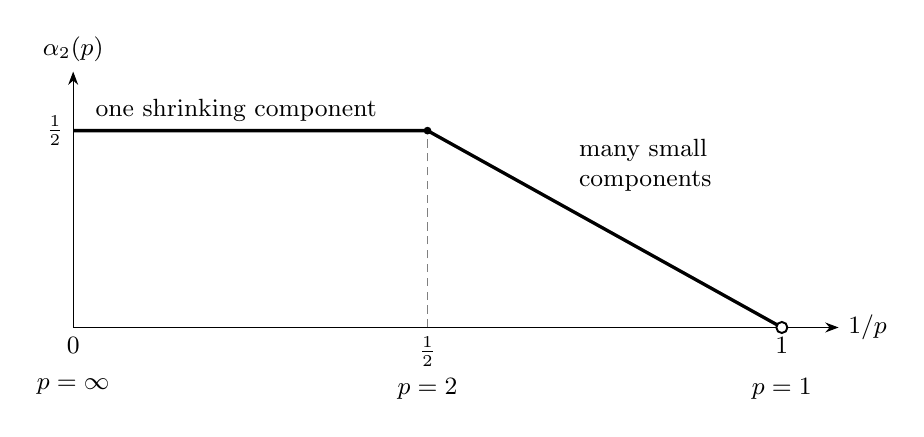
\begin{tikzpicture}[x=9cm,y=5cm,>=Stealth,font=\small]
 \draw[->] (0,0)--(1.08,0) node[right] {\(1/p\)};
 \draw[->] (0,0)--(0,.65) node[above] {\(\alpha_2(p)\)};
 \draw[densely dashed,gray] (.5,0)--(.5,.5);
 \draw[line width=1.2pt] (0,.5)--(.5,.5)--(1,0);
 \fill (.5,.5) circle[radius=1.4pt];
 \draw[fill=white,line width=.7pt] (1,0) circle[radius=2pt];
 \node[below] at (0,0) {\(0\)};
 \node[below] at (.5,0) {\(\frac12\)};
 \node[below] at (1,0) {\(1\)};
 \node[left] at (0,.5) {\(\frac12\)};
 \node[above] at (.23,.5) {one shrinking component};
 \node[above right,align=left] at (.70,.32) {many small\\components};
 \node[below=15pt] at (.5,0) {\(p=2\)};
 \node[below=15pt] at (0,0) {\(p=\infty\)};
 \node[below=15pt] at (1,0) {\(p=1\)};
\end{tikzpicture}
\caption{The sharp planar torsion exponent, plotted against \(1/p\).
The horizontal branch is forced by a single shrinking deleted
component; the sloping branch by many small deleted components.
The bounds hold for all finite-area nested open sets with uniformly
bounded outer area.  Matching examples keep the outer area and
ground-state eigenvalue fixed.  The endpoint \(p=1\) is excluded
because trace-class membership can fail.}
\label{fig:sharp-exponent}
\end{figure}



\section{Overlap torsion and the cost of nested comparisons}
\label{op:overlap-paths}

The quantity $\Gamma(D,E)$ in \eqref{op:overlap-def} has an exact
interpretation in terms of nested domain changes.  The underlying
torsional supermodularity is classical
\cite{LuttingerFriedberg1976}, as is the associated
valuation-metric construction \cite{Leclerc2003}; the following
variational proof specifies it for the actual Dirichlet form spaces
used here.

For nonnegative $u\in H_0^1(D)$ and $v\in H_0^1(E)$, the functions
$\min(u,v)$ and $\max(u,v)$ belong respectively to
$H_0^1(D\cap E)$ and $H_0^1(D\cup E)$.
This follows from the quasi-continuous characterization of
$H_0^1$ by vanishing quasi-everywhere off the open set, or by
approximation and the Sobolev lattice identities.
For $J(u)=\frac12\int\abs{\nabla u}^2-\int u$ those identities give
\[
 J(\min(u,v))+J(\max(u,v))=J(u)+J(v).
\]
Take $u=w_D$, $v=w_E$ and minimize on the intersection and union
to obtain
\begin{equation}\label{op:supermodular}
 T(D\cup E)+T(D\cap E)\ge T(D)+T(E).
\end{equation}
Applying this inequality to $D\cap F$ and $E\cap F$, and then
using monotonicity, gives
\[
 T(D\cap F)+T(E\cap F)
 \le T((D\cup E)\cap F)+T(D\cap E\cap F)
 \le T(F)+T(D\cap E).
\]
Rearrangement proves the triangle inequality
\begin{equation}\label{op:overlap-triangle}
 \Gamma(D,E)\le\Gamma(D,F)+\Gamma(F,E).
\end{equation}
Thus $\Gamma$ is a pseudometric on finite-volume open sets.

For a finite chain $D=D_0,D_1,\ldots,D_N=E$ in which every
consecutive pair is nested in either direction, assign cost
\[
 \mathcal C(D_0,\ldots,D_N)
     =\sum_{i=1}^N\abs{T(D_i)-T(D_{i-1})}.
\]
On a nested pair, $\Gamma$ is precisely this absolute torsion
difference.  Repeated application of \eqref{op:overlap-triangle}
therefore bounds every chain cost from below by $\Gamma(D,E)$.
The chain $D,D\cap E,E$ attains that bound.  Consequently
\begin{equation}\label{op:exact-path-cost}
 \boxed{\quad
 \Gamma(D,E)=\min_{\substack{\text{finite nested chains}\\D\leadsto E}}
          \mathcal C(D_0,\ldots,D_N).
 \quad}
\end{equation}
The chain space includes the empty domain with torsion zero, and
intermediate volumes are allowed to vary.

The ordinary torsion-function distance
$\gamma(D,E)=\int_{\R^n}\abs{w_D-w_E}\dd x$ obeys
\begin{equation}\label{op:gamma-comparison}
 \gamma(D,E)\le\Gamma(D,E),\qquad
 \Gamma(D,E)-\gamma(D,E)
   =2\int_{\R^n}\bigl(\min(w_D,w_E)-w_{D\cap E}\bigr)\dd x.
\end{equation}
Equality holds for nested pairs.  The nonnested estimates above
use $\Gamma$, the exact additive cost in
\eqref{op:exact-path-cost}; \eqref{op:gamma-comparison} has the
opposite direction from a bound that would replace it by $\gamma$.

\section{An exact class of torsion-controlled spectral filters}
\label{op:filters}

The critical trace comparison characterizes which continuous
functions of the reciprocal eigenvalues admit a uniform linear
torsion bound.  Let $\psi:[0,\infty)\to\R$ be continuous with
$\psi(0)=0$, and define the extended nonnegative sum
\[
 D_\psi(D,E)=\sum_{j\ge1}
       \abs{\psi(\mu_j(D))-\psi(\mu_j(E))}.
\]
Put
\begin{equation}\label{op:filter-L}
 L_\psi=\sup_{\substack{u,v\ge0\\u\ne v}}
       \frac{\abs{\psi(u)-\psi(v)}}{\abs{u^r-v^r}}.
\end{equation}
Equivalently, $L_\psi$ is the Lipschitz constant of
$s\mapsto\psi(s^{1/r})$.  A finite constant $C_\psi$ satisfying
\begin{equation}\label{op:filter-property}
 D_\psi(A,D)\le C_\psi\bigl(T(D)-T(A)\bigr)
 \quad\hbox{for every nested finite-volume pair }A\subset D
\end{equation}
exists if and only if $L_\psi<\infty$.
Writing $\lambda_B=\lambda_1(B_1)$ and $t_n=T(B_1)$, its best
constant satisfies
\begin{equation}\label{op:filter-best}
 \frac{L_\psi}{t_n\lambda_B^r}
       \le C_{\psi,\mathrm{opt}}\le c_nL_\psi.
\end{equation}

For sufficiency, monotonicity of the ordered reciprocal eigenvalues
gives
\[
 \abs{\psi(\mu_j(D))-\psi(\mu_j(A))}
 \le L_\psi\bigl(\mu_j(D)^r-\mu_j(A)^r\bigr).
\]
Summation and \eqref{op:critical-bound} prove the upper bound in
\eqref{op:filter-best}.  Furthermore
$\abs{\psi(x)}\le L_\psi x^r$, so
\begin{equation}\label{op:filter-summable}
 \sum_j\abs{\psi(\mu_j(D))}
 \le L_\psi\Tr R_D^r<\infty.
\end{equation}
Absolute summability is thus a consequence, not an assumption about
cancellation between two spectra.

For necessity, fix $0\le u<v$ and let
$a=\sqrt{u\lambda_B}$, $b=\sqrt{v\lambda_B}$.
Take concentric balls $A=B_a$, $D=B_b$, with $A=\varnothing$
when $u=0$.  Scaling gives
\[
 \mu_1(A)=u,\qquad\mu_1(D)=v,\qquad
 T(D)-T(A)=t_n\lambda_B^r(v^r-u^r).
\]
The first summand of \eqref{op:filter-property} therefore yields
$\abs{\psi(v)-\psi(u)}
 \le C_\psi t_n\lambda_B^r(v^r-u^r)$.
Taking the supremum proves necessity and the lower bound in
\eqref{op:filter-best}.

\subsection{Fixed outer volume and nonmonotone filters}
\label{op:fixed-volume-filters}

For $V>0$, let $B_V$ be a ball of volume $V$ and put
$M_V=\lambda_1(B_V)^{-1}$.  The corresponding exact characterization
for pairs with $\abs D=V$ replaces \eqref{op:filter-L} by
\begin{equation}\label{op:restricted-L}
 L_{\psi,V}=\sup_{\substack{0\le u,v\le M_V\\u\ne v}}
       \frac{\abs{\psi(u)-\psi(v)}}{\abs{u^r-v^r}}<\infty.
\end{equation}
The best constant lies between
$L_{\psi,V}/(t_n\lambda_B^r)$ and $c_nL_{\psi,V}$.
For sufficiency, Faber--Krahn gives
$\mu_j(A)\le\mu_j(D)\le M_V$, so the preceding proof uses only
the restricted interval.

For necessity, fix $0<u<v\le M_V$ and the concentric balls
$B_a\subset B_b$ used above.  If $W=V-\abs{B_b}>0$, choose
an integer $N$ so large that a ball of volume $W/N$ has first
reciprocal eigenvalue below $u$.  Place $N$ such balls disjointly
outside $B_b$, with union $P_N$, and set
\[
 A=B_a\mathbin{\dot\cup}P_N,
 \qquad D=B_b\mathbin{\dot\cup}P_N.
\]
Now $\abs D=V$, the largest reciprocal eigenvalues remain $u,v$,
and the common torsion contribution of $P_N$ cancels.  The same
first-coordinate test proves the required quotient bound.
When $W=0$ no padding is needed.  Continuity of $\psi$ supplies
the endpoint $u=0$ by letting $u\downarrow0$.
This proves the exactly fixed-volume statement.  Since sufficiency
holds for every $\abs D\le V$ and necessity already holds at
equality, the same characterization applies under the volume upper
bound.

The condition controls oscillation as well as decay.  For instance,
$\psi(x)=x^r\sin(1/x)$ for $x>0$, with $\psi(0)=0$, satisfies
$\abs{\psi(x)}\le x^r$, but
\[
 \frac{\psi'(x)}{rx^{r-1}}
     =\sin(1/x)-\frac1{rx}\cos(1/x)
\]
is unbounded near zero.  It therefore fails
\eqref{op:filter-property} even at fixed outer volume, despite
absolute summability of each transformed spectrum.
In contrast, $x^r\sin(\log x)$, extended by zero, has bounded
weighted derivative and is an admissible nonmonotone filter.
For powers $\psi(x)=x^q$, the global condition holds precisely
when $q=r$; on the fixed-volume interval it holds for $q\ge r$,
with $L_{\psi,V}=(q/r)M_V^{q-r}$.

For arbitrary pairs, the critical coordinate comparison gives
\begin{equation}\label{op:filter-arbitrary}
 D_\psi(D,E)\le c_nL_\psi\Gamma(D,E),
\end{equation}
and the restricted constant can be used when both volumes are at
most $V$.  Although \eqref{op:filter-summable} makes each
$\psi(R_D)$ trace class, these estimates concern ordered scalar
coordinates and scalar traces.  They do not identify the trace norm
of $\psi(R_D)-\psi(R_E)$, whose operators need not commute.

\subsection{Heat traces and spectral thresholds}
\label{op:heat-filters}

For a differentiable filter on $(0,\infty)$, continuous at zero,
the change of variables $s=x^r$ and the mean value theorem give
\begin{equation}\label{op:derivative-L}
 L_\psi=\sup_{x>0}\frac{\abs{\psi'(x)}}{rx^{r-1}},
\end{equation}
whenever this supremum is finite; the equality follows also in the
reverse direction by difference quotients.
For $t>0$, take $\psi_t(0)=0$ and
$\psi_t(x)=e^{-t/x}$ for $x>0$.  Then
\[
 \frac{\psi_t'(x)}{rx^{r-1}}
 =\frac{t^{-r}}r (t/x)^{r+1}e^{-t/x},
\]
whose maximum occurs at $t/x=r+1$.  Hence
\begin{equation}\label{op:heat-filter-bound}
 0\le Z_D(t)-Z_A(t)
 \le c_n\frac{(r+1)^{r+1}}{re^{r+1}}\,t^{-r}\delta,
 \qquad A\subset D,
\end{equation}
and, for arbitrary pairs,
\begin{equation}\label{op:heat-filter-pair}
 \sum_j\abs{e^{-t\lambda_j(D)}-e^{-t\lambda_j(E)}}
 \le c_n\frac{(r+1)^{r+1}}{re^{r+1}}\,t^{-r}\Gamma(D,E).
\end{equation}
The coefficient in dimension two is $27/(\pi e^3)$.

The continuous filters in this class also distinguish stability of
smoothed spectral quantities from stability of a sharp count.
Fix $a>0$ and let $s_0=\sqrt{a\lambda_B}$.
For $A_\varepsilon=B_{s_0-\varepsilon}$ and
$D_\varepsilon=B_{s_0+\varepsilon}$, the first reciprocal
eigenvalue crosses $a$, while the second remains below $a$ for
sufficiently small $\varepsilon>0$.  Thus the number of Laplacian
eigenvalues at most $1/a$ changes from zero to one, whereas
$T(D_\varepsilon)-T(A_\varepsilon)\to0$.
Even within smooth connected nested domains in one bounded ball,
a sharp count therefore has no uniform torsion modulus tending to
zero without separation from its spectral threshold.

\subsection{Regularized Fredholm determinants and their exact order range}
\label{op:determinants}

Let $m$ be a positive integer and $z>0$.  For a nonempty finite-volume
open set $D$, its inverse belongs to $\mathcal S_m$ exactly when
$m>d$.  Sufficiency follows from \eqref{op:mellin}; necessity
follows from the interior-cube argument in
Section~\ref{op:sharpness}.  Assume $m>d$ and define
\begin{equation}\label{op:det-filter}
 \psi_{m,z}(x)=\log(1+zx)
       +\sum_{k=1}^{m-1}\frac{(-1)^k(zx)^k}{k},\qquad x\ge0.
\end{equation}
The standard regularized Fredholm convention
\cite{BritzEtAl2021} is
\begin{equation}\label{op:det-product}
 \det_m(I+zR_D)=\prod_j\left[(1+z\mu_j(D))
     \exp\left(\sum_{k=1}^{m-1}
                   \frac{(-1)^k(z\mu_j(D))^k}{k}\right)\right].
\end{equation}
To verify convergence and fix the sign, differentiation gives
\begin{equation}\label{op:det-remainder}
 \psi_{m,z}(x)=(-1)^{m-1}z^m
       \int_0^x\frac{u^{m-1}}{1+zu}\dd u,
 \qquad
 \abs{\psi_{m,z}(x)}\le\frac{z^m x^m}{m}.
\end{equation}
Thus $\sum_j\abs{\psi_{m,z}(\mu_j(D))}<\infty$, and the
product in \eqref{op:det-product} converges to a strictly positive
number, independently of ordering.  In fact
$\sum_j\abs{e^{\psi_{m,z}(\mu_j(D))}-1}<\infty$, since
the summable logarithms form a bounded sequence.  Therefore
\[
 (I+zR_D)\exp\left(\sum_{k=1}^{m-1}
                     \frac{(-1)^k(zR_D)^k}{k}\right)-I
\]
is trace class and its ordinary Fredholm determinant is
\eqref{op:det-product}.  Its real logarithm is
\begin{equation}\label{op:log-det}
 F_{m,z}(D)=\log\det_m(I+zR_D)
           =\sum_j\psi_{m,z}(\mu_j(D)).
\end{equation}
The regularizing cancellation takes place inside
$\psi_{m,z}$ before summation; separate lower-power traces need
not exist.  Zero-extension kernel directions contribute factors one.

Convergence is weaker than linear torsion stability.  Put
$\alpha=m-r$.  Formula \eqref{op:derivative-L} gives
\[
 L_{m,z}=\frac{z^r}{r}
       \sup_{y>0}\frac{y^\alpha}{1+y}.
\]
This supremum is finite precisely for $0\le\alpha\le1$.
Define
\[
 b_\alpha=
 \begin{cases}
  1,&\alpha=0\ \hbox{or}\ \alpha=1,\\
  \alpha^\alpha(1-\alpha)^{1-\alpha},&0<\alpha<1.
 \end{cases}
\]
For $0<\alpha<1$ the maximizing point is
$y=\alpha/(1-\alpha)$; at the two endpoints the supremum is one.
It follows that for every integer $r\le m\le r+1$,
\begin{equation}\label{op:det-stability}
 0\le(-1)^{m-1}\bigl(F_{m,z}(D)-F_{m,z}(A)\bigr)
 \le\frac{c_n}{r}b_{m-r}z^r\delta,
 \qquad A\subset D.
\end{equation}
The absolute arbitrary-pair difference has the same upper bound
with $\delta$ replaced by $\Gamma(D,E)$; so does the sum of
absolute differences of the individual ordered logarithmic factors.
Indeed, \eqref{op:det-remainder} makes the filter monotone with
sign $(-1)^{m-1}$, so the nested trace difference has no
cancellation.

These integer orders are exactly those admitting a domain-independent
linear torsion estimate for the scalar logarithm.  To prove necessity
directly at the trace level, let $\beta=\mu_1(B_1)$.
If $d<m<r$, then
\[
 \abs{F_{m,z}(B_\varepsilon)}
 \ge\abs{\psi_{m,z}(\beta\varepsilon^2)}
 \sim\frac{z^m\beta^m}{m}\varepsilon^{2m},
 \qquad T(B_\varepsilon)=t_n\varepsilon^{2r}.
\]
Their ratio diverges as $\varepsilon\downarrow0$.
If $m>r+1$, the asymptotic formula
\[
 \abs{\psi_{m,z}(x)}
       \sim\frac{z^{m-1}}{m-1}x^{m-1}
       \qquad(x\to\infty)
\]
and the first coordinate on $B_L$, $L\to\infty$, give a ratio
bounded below by a positive constant times $L^{2(m-1-r)}$.
All logarithmic factors have the same sign, which justifies both
first-coordinate lower bounds.  Empty inner domains already suffice
for these tests.

Under $\abs D\le V$, the reciprocal range is restricted to
$[0,M_V]$.  The derivative ratio is then bounded exactly when
$m\ge r$, and one may use
\begin{equation}\label{op:det-local-L}
 L_{m,z;V}\le\frac{z^m}{r}M_V^{m-r}.
\end{equation}
The excluded orders $d<m<r$ fail even when $\abs D=V$ exactly
and the inner domain is nonempty.  Choose disjoint balls
$C_\varepsilon$ and $B_\varepsilon$ with
$\abs{C_\varepsilon}=V-\abs{B_\varepsilon}$ and set
$A_\varepsilon=C_\varepsilon$,
$D_\varepsilon=C_\varepsilon\mathbin{\dot\cup}B_\varepsilon$.
They fit in one fixed bounded cube for small $\varepsilon$.
Torsion and the absolutely convergent sum \eqref{op:log-det} are
additive on disjoint components, leaving exactly the diverging
small-ball ratio above.

Consequently, if $n=2k$, the smallest convergent order is $k+1$,
the globally stable orders are $k+1,k+2$, and all orders $m\ge k+1$
are stable under a volume bound.  If $n=2k+1$, these three answers
are respectively $k+1$, $k+2$, and $m\ge k+2$.
In particular, the smallest stable choice is $m=\lceil r\rceil$,
which need not be the smallest convergent choice.  In the plane,
\eqref{op:det-stability} with $m=r=2$ reads
\begin{equation}\label{op:planar-det}
 0\le\log\det_2(I+zR_A)-\log\det_2(I+zR_D)
       \le\frac{z^2}{\pi}\delta.
\end{equation}
At $z=0$ all products equal one and all logarithmic differences
vanish.  These are regularized Fredholm determinants of bounded
resolvent perturbations; their construction requires neither a
spectral-zeta continuation nor a zeta-regularized Laplacian
determinant on the domain.



\section{Low-energy comparison and the two forms of spectral surgery}
\label{surgery:resolvents}

We now turn to finite geometric replacements in the plane.  The
whole-spectrum estimates and the construction below use the same
torsion defect, but they serve different purposes.  For a prescribed
energy window, the compression of a resolvent difference has norm and
trace bounded \emph{linearly} in the torsion loss.  This linear estimate
allows removed area to pay for spectral error, or for a loss of rank.
Using only a whole-operator Schatten bound would lose this quantitative
balance.  We give the low-energy argument explicitly before applying it
to the finite catalogues.

\subsection{A linear comparison on the entire low-energy subspace}

Let \(A\subset D\) be bounded open subsets of \(\R^2\), with \(D\ne
\varnothing\).  We allow \(A=\varnothing\) temporarily.  The Dirichlet
realization is always the one associated with \(H^1_0\) of the actual
open set.  In particular, a slit is not removed merely because it has
zero area.  Extend the resolvent of \(A\) by zero to \(L^2(D)\), and put
\[
 R_D=(-\Delta_D)^{-1},\qquad R_A=(-\Delta_A)^{-1},\qquad
 S=R_D-R_A,
\]
with \(R_\varnothing=0\).  These are compact self-adjoint operators;
extension may introduce an infinite-dimensional zero eigenspace.
Write
\begin{equation}
 \begin{gathered}
 w_D=R_D1,\qquad T(D)=\int_D w_D\,\dd x,\\
 \mathcal E(D)=-\frac12T(D),\qquad
 \Delta=\mathcal E(A)-\mathcal E(D)
        =\frac{T(D)-T(A)}2.
 \end{gathered}
 \label{surgery:torsion}
\end{equation}
Here and below functions on a smaller open set are extended by zero
when they occur in an integral on a larger one.

Two positivity properties of \(S\) will be used separately.  First,
\[
 \langle f,R_Df\rangle
 =\sup_{v\in H^1_0(D)}
       \left(2\langle f,v\rangle-\int_D\abs{\nabla v}^2\,\dd x\right)
\]
and the inclusion \(H^1_0(A)\subset H^1_0(D)\) show that \(S\) is positive
semidefinite.  Second, weak comparison gives
\begin{equation}
 f\ge0\quad\Longrightarrow\quad Sf\ge0\quad\hbox{almost everywhere}.
 \label{surgery:order}
\end{equation}
For completeness, both resolvent solutions for such \(f\) are
nonnegative.  The test function
\((R_Af-R_Df)_+\) belongs to \(H^1_0(A)\): approximate \(R_Af\) by
compactly supported functions in \(A\), take the positive part after
subtracting the nonnegative zero extension of \(R_Df\), and use
continuity of truncation in \(H^1\).  Subtracting the two weak equations
and testing with this function proves that its gradient vanishes.
This proves \eqref{surgery:order} even for rough or disconnected sets.
Positive semidefiniteness alone would not imply this order property.

If \(v\) is a bounded real function, order preservation gives
\[
 \abs{Sv}\le S\abs v\le \norm v_\infty S1.
\]
Since \(S1=w_D-w_A\ge0\), it follows that
\begin{equation}
 0\le \langle v,Sv\rangle
 \le \norm v_\infty^2\int_D(w_D-w_A)\,\dd x
 =2\norm v_\infty^2\Delta.
 \label{surgery:bounded-quadratic}
\end{equation}
All the estimates can therefore be obtained without selecting a
pointwise representative of a difference of Green kernels.

Choose real orthonormal Dirichlet eigenfunctions \(u_i\) on \(D\),
ordered with multiplicity, and let \(V_j=\operatorname{span}
\{u_1,\ldots,u_j\}\).  At a multiple endpoint any required number of
orthonormal states may be chosen.  The Dirichlet heat semigroup is
dominated by the free heat semigroup on every open set
\cite{Davies1989}.  Its diagonal expansion consequently gives, for
almost every \(x\in D\) and \(t>0\),
\[
 \rho_j(x):=\sum_{i=1}^j u_i(x)^2
 \le e^{t\lambda_j(D)}p_D(t;x,x)
 \le \frac{e^{t\lambda_j(D)}}{4\pi t}.
\]
Taking \(t=\lambda_j(D)^{-1}\), and applying Cauchy--Schwarz to the
finite expansion of a function in \(V_j\), yields
\begin{equation}
 \rho_j\le\frac{e\lambda_j(D)}{4\pi},
 \qquad
 \norm v_\infty^2\le
       \frac{e\lambda_j(D)}{4\pi}\norm v_2^2
       \quad(v\in V_j).
 \label{surgery:heat-projector}
\end{equation}
This estimates the whole spectral projector, rather than adding
separate bounds for the suprema of its eigenfunctions.

Let \(P_j\) denote the orthogonal projection onto \(V_j\).
Equations \eqref{surgery:bounded-quadratic} and
\eqref{surgery:heat-projector}, together with positivity, give
\begin{equation}
 \norm{P_jSP_j}_{L^2\to L^2}
 \le \frac{e\lambda_j(D)}{2\pi}\Delta.
 \label{surgery:compressed-norm}
\end{equation}
On \(V_j\), the quadratic form of \(R_D\) is bounded below by
\(\lambda_j(D)^{-1}\) times the squared norm.  Descending
compact-operator min--max therefore shows that
\begin{equation}
 \frac1{\lambda_j(A)}
 \ge \frac1{\lambda_j(D)}
       -\frac{e\lambda_j(D)}{2\pi}\Delta
 \label{surgery:inverse}
\end{equation}
whenever the expression on the right is positive.  More precisely,
min--max first bounds the \(j\)-th descending eigenvalue of the
extended operator \(R_A\) by that expression.  Positivity then proves
the existence of \(j\) positive eigenvalues and justifies the
reciprocal notation.  Thus the argument also excludes an empty \(A\)
when a positive bound has been established; nonemptiness and rank
have not been assumed in advance.

The compressed-resolvent argument is already present in
\cite[Theorem~3.4 and Lemma~3.5]{Bucur2003}.  Its use in spectral
surgery, and simultaneous improvement of an initial spectrum, are
established antecedents \cite{Bucur2012,BucurMazzoleni2015}.
The order comparison and the classical heat-projector bound remove
the extra index factors that arise when eigenfunction suprema are
estimated separately.  We use their combination as an input to the
quantitative construction.  Its energy-dependent coefficient serves
a different purpose from a dimension-only whole-resolvent estimate.

\subsection{A trace estimate with the same energy dependence}
\label{surgery:trace-section}

There is a useful companion to \eqref{surgery:compressed-norm}.
For every bounded real \(f\), positivity preservation implies
\begin{equation}
 \abs{Sf}^2\le S1\,S(f^2)\quad\hbox{almost everywhere}.
 \label{surgery:positive-schwarz}
\end{equation}
Indeed, apply \(S\) to the nonnegative function \((f-z)^2\) for each
rational \(z\).  Outside one common null set,
\(S(f^2)-2zSf+z^2S1\ge0\) for all rational, hence all real, \(z\).
Its discriminant gives \eqref{surgery:positive-schwarz}; if \(S1=0\),
the same polynomial forces \(Sf=0\).  No division by \(S1\) is needed.

Suppose \(\lambda_k(D)\le E\), and put \(M=eE/(4\pi)\).  Then
\(\rho_k\le M\), and summing \eqref{surgery:positive-schwarz} gives
\[
 \sum_{i=1}^k\abs{Su_i}^2
 \le S1\,S(\rho_k)\le M(S1)^2.
\]
Pointwise Cauchy--Schwarz now yields
\[
 \sum_{i=1}^k u_iSu_i
 \le \rho_k^{1/2}
       \left(\sum_{i=1}^k\abs{Su_i}^2\right)^{1/2}
 \le M S1.
\]
Integrating, we obtain
\begin{equation}
 0\le\operatorname{Tr}(P_kSP_k)
 \le \frac{eE}{2\pi}\Delta.
 \label{surgery:trace}
\end{equation}
The trace is nonnegative by positive semidefiniteness, although its
pointwise summands need not be nonnegative.  The important feature is
that summing the states has not introduced a further factor \(k\).

\section{Torsion minimization with an open positivity set}
\label{surgery:minimization}

We next give the existence and perimeter arguments needed for the
particular penalties used below.  Let \(D\) be a bounded nonempty
planar open set with compact smooth boundary, not necessarily
connected, and let \(c>0\).  Smooth boundary here has its usual domain
meaning: locally the domain lies on one side of a smooth embedded
curve.  Minimize, over nonnegative \(u\in H^1_0(D)\),
\begin{equation}
 J_c(u)=\frac12\int_D\abs{\nabla u}^2\,\dd x
            -\int_Du\,\dd x+c\abs{\{u>0\}}.
 \label{surgery:functional}
\end{equation}
This standard torsion-plus-volume construction underlies
\cite{Bucur2012,BucurMazzoleni2015}.  The details below ensure that the
minimizer used here is an open set for every \(c>0\), rather than an
unspecified quasi-open representative.

Poincare and Cauchy--Schwarz make \(J_c\) coercive.  A minimizing
sequence has a subsequence converging weakly in \(H^1_0(D)\), strongly
in \(L^2(D)\), and almost everywhere.  Its limit \(u\) is nonnegative.
The Dirichlet integral is weakly lower semicontinuous, the linear
term converges, and
\[
 1_{\{u>0\}}\le\liminf_n1_{\{u_n>0\}}
 \quad\hbox{almost everywhere}.
\]
Fatou's lemma proves lower semicontinuity of the volume term.
Thus \(u\) minimizes \eqref{surgery:functional}.

To obtain continuity, fix a ball \(B_r(x)\Subset D\), and let \(h\)
be the harmonic function with the same Sobolev trace as \(u\) on
that ball.  The weak maximum principle gives \(h\ge0\).  Replace \(u\)
by \(h\) in the ball.  Harmonic orthogonality and minimality, with
\(X=\norm{\nabla(u-h)}_{L^2(B_r)}\), imply
\[
 \frac12X^2
 \le \int_{B_r}\abs{u-h}\,\dd x+c\abs{B_r}.
\]
Poincare on the ball and Cauchy--Schwarz bound the integral by
\(C r^2X\).  Young's inequality therefore gives
\begin{equation}
 X^2\le C(c+r^2)r^2.
 \label{surgery:harmonic-replacement}
\end{equation}
Here and in this continuity argument \(C\) is an absolute constant,
whose value does not enter any subsequent catalogue bound.
For \(F_x(r)=\int_{B_r(x)}\abs{\nabla u}^2\), harmonic energy
minimality and the mean-value inequality for \(\abs{\nabla h}^2\)
then give
\[
 F_x(\rho)\le 2(\rho/r)^2F_x(r)+C(c+r^2)r^2,
 \qquad 0<\rho<r.
\]
Fix \(0<\alpha<1\), and choose \(0<\theta<1\) with
\(2\theta^2\le\frac12\theta^{2\alpha}\).
Iteration on radii \(r,\theta r,\theta^2r,\ldots\) gives
\(F_x(\rho)\le C_{K,\alpha}\rho^{2\alpha}\), uniformly for centers
in a compact subset \(K\Subset D\) and small radii.  The geometric
series converges because \(2-2\alpha>0\).  Poincare on balls gives
the corresponding mean-oscillation bound
\[
 \int_{B_\rho(x)}
       \abs{u-u_{B_\rho(x)}}^2\,\dd x
       \le C_{K,\alpha}\rho^{2+2\alpha}.
\]
The Morrey--Campanato conclusion, obtained by telescoping averages
over nested balls, supplies a locally \(C^{0,\alpha}\)
representative.  Only this continuity, not free-boundary
Lipschitz regularity, is required.

The torsion function \(w_D\) is positive in each component and,
because \(D\) has smooth boundary, is continuous on \(\overline D\)
and vanishes there on \(\partial D\).  For
\(F(v)=\frac12\int\abs{\nabla v}^2-\int v\), its weak equation gives
the exact identity
\[
 F(v)=F(w_D)+\frac12\norm{\nabla(v-w_D)}_2^2,
 \qquad v\in H^1_0(D).
\]
Compare \(u\) with \(v=\min(u,w_D)\).  Their positivity sets agree
up to null sets, and hence
\[
 J_c(u)-J_c(v)
 =\frac12\norm{\nabla(u-w_D)_+}_2^2.
\]
Minimality forces \(u\le w_D\).  Local continuity makes this a
pointwise inequality in \(D\), so the representative of \(u\)
extended by zero is continuous across \(\partial D\).  Consequently
\[
 A=\{u>0\}
\]
is a bounded open subset of \(D\).

For \(s>0\), the support of \((u-s)_+\) lies in the compact set
\(\{u\ge s\}\Subset A\).  Local mollification therefore puts
\((u-s)_+\) in \(H^1_0(A)\).  These truncations converge to \(u\)
in \(H^1\) as \(s\downarrow0\); the gradient of \(u\) is zero almost
everywhere on \(\{u=0\}\).  Thus \(u\in H^1_0(A)\).
On the support of any \(\varphi\in C^\infty_c(A)\), \(u\) has a
strictly positive minimum.  Both signs of a sufficiently small
variation \(u+t\varphi\) leave the positivity set unchanged.
Differentiating \eqref{surgery:functional} gives
\[
 \int_A\nabla u\cdot\nabla\varphi\,\dd x
 =\int_A\varphi\,\dd x.
\]
Density and uniqueness identify \(u=w_A\).  If \(u=0\), take
\(A=\varnothing\).  For every open \(B\subset D\), the zero-extended
torsion function \(w_B\) is an admissible competitor and is positive
in \(B\), component by component.  It follows that
\begin{equation}
 \mathcal E(A)+c\abs A
 \le \mathcal E(B)+c\abs B
 \quad\hbox{for every open }B\subset D.
 \label{surgery:set-minimum}
\end{equation}
We have also retained the stronger function-competitor minimality
used in the next calculation.

\subsection{Perimeter control by truncation}
\label{surgery:perimeter-section}

Put \(a=\abs A\) and compare \(u=w_A\) with \((u-s)_+\) in
\eqref{surgery:functional}.  The exact energy difference gives
\[
 \frac12\int_{\{0<u\le s\}}\abs{\nabla u}^2\,\dd x
       +c\abs{\{0<u\le s\}}
 \le \int_A\min(u,s)\,\dd x\le sa.
\]
Bounding the two nonnegative terms separately and applying
Cauchy--Schwarz yields
\[
 \int_{\{0<u\le s\}}\abs{\nabla u}\,\dd x
 \le \sqrt{2/c}\,sa.
\]
The coarea formula supplies levels \(s_n\downarrow0\) with
\(\operatorname{Per}(\{u>s_n\})\le\sqrt{2/c}\,a\).
Their indicators converge in \(L^1\) to \(1_A\).
Lower semicontinuity of De Giorgi perimeter proves
\begin{equation}
 \operatorname{Per}(A)\le\sqrt{\frac2c}\,\abs A.
 \label{eq:perimeter}
\end{equation}
This is the established truncation argument of
\cite[Theorem~2.2]{Bucur2012}; coarea and lower semicontinuity of
perimeter are standard \cite{EvansGariepy2015}.  The perimeter in
\eqref{eq:perimeter} is not being identified with the length of an
arbitrary topological boundary.

\subsection{Preserving a prefix, or paying for a loss of rank}
\label{surgery:two-outputs}

First suppose that \(D\) has area one and
\(\lambda_m(D)\le H\), and choose \(c=H^{-2}\).
With \(a=\abs A\) and \(t=1-a\), domain monotonicity and comparison
with \(D\) in \eqref{surgery:set-minimum} give
\[
 0\le\Delta\le ct.
\]
For \(j\le m\), \eqref{surgery:inverse} has the positive right-hand
side
\[
 \frac{1-\kappa_jt}{\lambda_j(D)},\qquad
 \kappa_j=\frac{e\lambda_j(D)^2}{2\pi H^2}
 \le\frac e{2\pi}<\frac12.
\]
In particular \(A\ne\varnothing\).  Since \(0<a\le1\) and
\(\kappa_j\le1\),
\[
 a\lambda_j(A)
 \le \frac{1-t}{1-\kappa_jt}\lambda_j(D)
 \le\lambda_j(D).
\]
For \(S_0=a^{-1/2}A\), planar scaling and
\eqref{eq:perimeter} give the simultaneous conclusion
\begin{equation}
 \abs{S_0}=1,\qquad
 \lambda_j(S_0)\le\lambda_j(D)\quad(1\le j\le m),\qquad
 \operatorname{Per}(S_0)\le\sqrt2\,H.
 \label{surgery:prefix}
\end{equation}
No gap between consecutive eigenvalues is involved.

The second output permits a loss of rank and will be used only for
the scalar ratio \(\abs D\lambda_k(D)/k\).
Let \(D\) again be smooth with \(\abs D=1\), assume
\(\lambda_k(D)\le E\), fix \(0<\eta\le1\), and choose
\[
 c=\frac{k\eta}{4E^2}.
\]
For its minimizing set, let \(a=\abs A\), \(t=1-a\).
The trace bound \eqref{surgery:trace} gives
\[
 \operatorname{Tr}(P_kSP_k)
 \le\frac{eE}{2\pi}\Delta\le Ect.
\]
Inside \(V_k\), discard the eigenvectors of the positive compression
\(P_kSP_k\) whose eigenvalues are strictly greater than
\(s=\eta/((1+\eta)E)\).  The retained dimension \(r\) is an integer,
and counting the discarded eigenvalues by their contribution to
the trace gives
\[
 r\ge k-\frac{\operatorname{Tr}(P_kSP_k)}s
 \ge k-\frac{(1+\eta)E^2ct}{\eta}
 =k\left(1-\frac{1+\eta}{4}t\right)
 \ge\frac{k(1+a)}2.
\]
On this retained subspace the quadratic form of \(R_A\) is at least
\(1/E-s=1/((1+\eta)E)\).  Resolvent min--max proves all assertions
in
\begin{equation}
 \begin{gathered}
  0<a\le1,\qquad r\in\{1,\ldots,k\},\qquad
  r\ge\frac{k(1+a)}2,\qquad
  \lambda_r(A)\le(1+\eta)E,\\
  \frac ar\le\frac1k,\qquad
  \frac{a\lambda_r(A)}r\le(1+\eta)\frac Ek.
 \end{gathered}
 \label{eq:trace-rank}
\end{equation}
Indeed \(r\ge k/2>0\) proves nonemptiness, and
\(a/r\le2a/(k(1+a))\le1/k\).
Repeated eigenvalues and equality at the truncation threshold cause
no difficulty.  The same set satisfies \eqref{eq:perimeter} with
the chosen \(c\).  It is the saved physical area, not a substitute
spectral mass, that compensates for the discarded rank.

\section{Inner regularization and hole-uniform grid covering}
\label{grid:construction}

\subsection{One family of compact trials for every prefix}
\label{surgery:compact-trials}

Let \(\Om\) be any bounded nonempty open set and fix \(m\) and \(b>0\).
Approximate its first \(m\) real eigenfunctions in \(H^1_0(\Om)\)
by \(f_1,\ldots,f_m\in C^\infty_c(\Om)\).  The mass and energy Gram
matrices of this family approach \(I\) and
\(\operatorname{diag}(\lambda_1,\ldots,\lambda_m)\), respectively.
To make the simultaneous assertion explicit, choose the
approximations so that both operator-norm errors are at most
\(\delta\), where
\[
 0<\delta\le\frac{b}{2(1+\lambda_m(\Om)+b)}.
\]
Every principal \(j\)-by-\(j\) compression has the same error bound.
Its mass matrix is at least \((1-\delta)I\), and its energy matrix
is at most \((\lambda_j(\Om)+\delta)I\).  Consequently every
first-\(j\) trial span is \(j\)-dimensional and has maximal
Rayleigh quotient at most
\[
 \frac{\lambda_j(\Om)+\delta}{1-\delta}
 \le\lambda_j(\Om)+b,\qquad 1\le j\le m.
\]

Let \(K\Subset\Om\) be the union of these compact supports.  Choose
\(\chi\in C^\infty_c(\Om)\), equal to one on a neighborhood of \(K\).
A regular level in \((0,1)\) gives a bounded smooth open set
\(\Om'\Subset\Om\) containing \(K\).  Thus
\begin{equation}
 \abs{\Om'}\le\abs{\Om},\qquad
 \lambda_j(\Om')\le\lambda_j(\Om)+b\quad(1\le j\le m).
 \label{surgery:inner}
\end{equation}
This approximation is made inside the original form domain.  It is
therefore valid in the presence of arbitrary boundary roughness,
disconnectedness, and positive-capacity slits.

\subsection{Positive torsion levels preserve the perimeter budget}
\label{surgery:bv-section}

The minimizers above admit a more precise regularization than an
arbitrary finite-perimeter set.  Let \(u=w_A\) be the continuous
minimizer of \eqref{surgery:functional}, assume \(a=\abs A>0\), and
put \(C_c=\sqrt{2/c}\,a\).  Interior elliptic regularity gives
\(u\in C^\infty(A)\), since \(-\Delta u=1\) there.  For every
\(t>0\), continuity of the zero extension shows that
\(\{u\ge t\}\) is a compact subset of \(A\).  A positive regular
superlevel \(G_t=\{u>t\}\) consequently has compact smooth boundary.

The truncation estimate already proved gives, for every \(s>0\),
\[
 \int_0^s\operatorname{Per}(G_t)\,\dd t
 =\int_{\{0<u<s\}}\abs{\nabla u}\,\dd x
 \le C_cs.
\]
Almost every positive value is regular by Sard's theorem.  Hence for
each \(s>0\) one can choose a positive regular \(t<s\) with
\(\operatorname{Per}(G_t)\le C_c\).  Choosing such values tending
to zero gives smooth inner sets with area tending to \(a\), all
with the same perimeter bound.  A compact smooth boundary has only
finitely many components, so these are precisely the smooth sets
needed for the planar covering argument below.

The convergence is also spectral.  Given a finite prefix and a
positive allowance, choose one simultaneous compact trial family
in \(A\) as above.  Its combined support \(K\) satisfies
\(\min_Ku>0\).  Every sufficiently small positive superlevel
contains all those trials.  Inclusion in \(A\) and min--max
therefore give
\[
 \lambda_j(A)\le\lambda_j(G_t)\le\lambda_j(A)+r
 \qquad(1\le j\le m)
\]
along sufficiently small selected levels.  In particular, every
fixed eigenvalue converges to its value on \(A\).  Nestedness of
the selected sequence is unnecessary.

After any dilation by \(\ell>0\), this proves the following form
used throughout the construction: for every \(m\) and \(r>0\)
there is a bounded smooth open set \(V\) such that
\begin{equation}
 \begin{gathered}
 \overline V\subset\ell A,\qquad
 \abs V\le\ell^2a,\qquad
 \operatorname{Per}(V)\le\ell\sqrt{2/c}\,a,\\
 \lambda_j(\ell A)\le\lambda_j(V)
           \le\lambda_j(\ell A)+r\quad(1\le j\le m).
 \end{gathered}
 \label{surgery:bv}
\end{equation}
The area can additionally be made arbitrarily close to
\(\ell^2a\) from below.  For the normalized prefix output
\(S_0=a^{-1/2}A\), the perimeter bound is at most \(\sqrt2H\).
For the area--rank output no dilation is made, and it is
\(\sqrt{2/c}\,a\).

This regularization is internal to the actual positivity set; it
does not fill a slit or charge an extra area allowance.  Its level
may depend on the source and the trial supports without a known
rate.  The catalogue requires only the uniform area and perimeter
outputs, not an algorithm reconstructing the regularized source.

\subsection{A lower bound and the active components}
\label{grid:active-section}

We shall use the elementary planar consequence of the Li--Yau
inequality \cite{LiYau1983},
\begin{equation}
 \abs{\Om}\lambda_j(\Om)\ge2\pi j,
 \qquad j\ge1.
 \label{grid:li-yau}
\end{equation}
Here is its Fourier proof on the precise open-set class in use.
Extend an orthonormal first-\(j\) eigenfamily by zero and take
\(\widehat u(\xi)=(2\pi)^{-1}\int e^{-ix\cdot\xi}u(x)\,\dd x\).
Bessel's inequality and Plancherel give, for
\(f=\sum_{i\le j}\abs{\widehat u_i}^2\),
\[
 0\le f\le M:=\frac{\abs{\Om}}{4\pi^2},\qquad
 \int_{\R^2}f\,\dd\xi=j,\qquad
 \int_{\R^2}\abs\xi^2f\,\dd\xi=\sum_{i\le j}\lambda_i(\Om).
\]
Choose \(R\) with \(M\pi R^2=j\).
The product
\((\abs\xi^2-R^2)(f-M1_{\{\abs\xi<R\}})\) is nonnegative.
After integration and cancellation of the equal masses this gives
\[
 \sum_{i\le j}\lambda_i(\Om)
 \ge M\frac{\pi R^4}{2}
 =\frac{2\pi j^2}{\abs{\Om}}.
\]
Bounding the sum above by \(j\lambda_j(\Om)\) proves
\eqref{grid:li-yau}.  No smoothness or connectedness has been used.

Suppose a smooth bounded open set \(V\) has
\(\lambda_m(V)\le F\).  Delete every whole component whose first
eigenvalue is strictly greater than \(F\), and call the resulting
union \(G\).  The Dirichlet operator is a direct sum over the open
components.  Removed components contribute no state at or below
\(F\), so all the first \(m\) ordered eigenvalues, including endpoint
multiplicities, are unchanged.  If \(q\) is the number of retained
components, \eqref{grid:li-yau} gives
\begin{equation}
 \lambda_j(G)=\lambda_j(V)\ (1\le j\le m),\qquad
 q\le\frac{\abs G F}{2\pi}\le\frac{\abs V F}{2\pi}.
 \label{grid:active-components}
\end{equation}
Area and perimeter do not increase.  Compact smooth boundary ensures
that only finitely many components and boundary curves occur.

\subsection{Covering without a charge for the number of holes}
\label{grid:hole-cover}

Let \(G\) have compact smooth boundary, \(q\) open components, and
perimeter \(p\).  For \(t>0\) put
\(G_t=\{x:\operatorname{dist}(x,G)<t\}\).
We first establish
\begin{equation}
 \abs{G_t}-\abs G\le(2+\pi)tp+\pi qt^2.
 \label{grid:tube}
\end{equation}
The number of holes does not appear in this estimate.

A compact rectifiable curve of length \(\ell\) has a radius-\(t\)
neighborhood of area at most \(2t\ell+\pi t^2\).
For a polygonal path, begin with the radius-\(t\) disk at its initial
point.  Adding a segment of length \(a\) adds at most \(2ta\),
because the disk at the starting endpoint is already covered.
Induction proves the assertion for a polygonal path, including a
closed one.  An inscribed polygonal approximation with subarcs of
length at most \(\delta\) has length at most \(\ell\) and Hausdorff
distance at most \(\delta\) from the curve.  Apply the polygonal
bound at radius \(t+\delta\) and let \(\delta\downarrow0\).

Each component of \(G\) has one outer Jordan boundary; its remaining
boundary curves bound holes.  An outer curve of length \(\ell\)
costs at most \(2t\ell+\pi t^2\), and there are exactly \(q\) such
curves.  For a hole with boundary length \(\ell>t\), its part within
distance \(t\) of that boundary costs at most
\[
 2t\ell+\pi t^2\le(2+\pi)t\ell.
\]
If instead \(\ell\le t\), pay for the whole Jordan interior.
Each coordinate span of the curve is at most \(\ell/2\), since
both arcs joining a coordinate minimum to a maximum have length
at least that span.  The hole lies in the resulting bounding box,
and therefore has area at most
\[
 \ell^2/4\le t\ell/4\le(2+\pi)t\ell.
\]
Every point of \(G_t\setminus G\) lies in one of these charged
regions: choose a component at distance less than \(t\), and
follow a segment to a nearby point in that component until it
crosses the relevant boundary curve.  Other components inside a
hole merely cause overcounting, which is harmless.  Summing the
charges proves \eqref{grid:tube}.  No reach, curvature bound, or
separation between boundary curves has been used.

Fix a square grid of pitch \(h>0\).  Select every closed grid
square that meets \(\overline G\), including all squares incident
to a contact on a grid edge or vertex, and let \(U\) be the interior
of their union.  Every point of \(\overline G\) is an interior point
of that union; compactness even gives a positive distance to \(U^c\).
Every selected cell is within distance \(\sqrt2h\) of \(\overline G\),
so \(U\subset G_{2\sqrt2h}\), with the factor two ensuring strict
neighborhood containment.  If \(N\) cells were selected, their
interiors are disjoint and all grid boundaries have zero area.
Consequently \eqref{grid:tube} gives
\begin{equation}
 \begin{gathered}
  \overline G\subset U,\qquad
  \abs U=Nh^2,\\
  \abs U\le\abs G+2\sqrt2(2+\pi)h\operatorname{Per}(G)
                       +8\pi qh^2,\qquad
  \lambda_j(U)\le\lambda_j(G)\quad(j\ge1).
 \end{gathered}
 \label{grid:outer-cover}
\end{equation}
The last assertion is Dirichlet form inclusion.  The new domain may
fill holes or join nearby components, but the entire added physical
area has been charged.  This construction is applied only to the
smooth set obtained from \eqref{surgery:bv}; no outer-tube estimate
for a rough finite-perimeter representative is being assumed.

\subsection{Retaining and packing physical components}
\label{grid:component-retention}

The domain \(U\) is a genuine grid mask: it is the interior of a
finite union of closed squares, with every common cell edge opened.
Its open components are exactly the edge-connected cell components.
If two closures meet only at a vertex, their open sets remain
disconnected.  Choose an ordered first-\(m\) orthonormal eigenfamily
of \(U\) from its componentwise direct-sum eigenbasis, and retain
precisely the components carrying these \(m\) states.  Their union
\(U_0\) has at most \(m\) components and
\begin{equation}
 \lambda_j(U_0)=\lambda_j(U)\quad(1\le j\le m).
 \label{grid:retained-spectrum}
\end{equation}
Indeed domain inclusion gives the inequality in one direction, and
the retained first-\(j\) trial spans give the reverse inequality.
At a multiple endpoint choose any allocation of the required
component-supported states.  Whole components are retained, with
their whole spectra, not just a selected eigenvalue list.

Dilate by \(h^{-1}\) to obtain unit cells.  An edge-connected
\(n\)-cell component has bounding-box width and height at most \(n\).
If the retained components have a total of \(N_0\) cells, translate
their boxes by integer vectors and place them horizontally with one
blank column between successive boxes.  Their union \(P\) fits in
a \(2N_0\)-by-\(N_0\) grid, since the total width is at most
\(N_0+q_0-1\le2N_0-1\).  Componentwise translations preserve the
entire Dirichlet direct-sum spectrum.  Finally, for the
area-one normalization \(P^\#=N_0^{-1/2}P\),
\begin{equation}
 \lambda_j(P^\#)=N_0\lambda_j(P)
                =\abs{U_0}\lambda_j(U_0).
 \label{grid:normalization}
\end{equation}
The normalization is of the whole packed union, not of each
component separately.

\section{A simultaneous finite grid replacement}
\label{grid:prefix-section}

Simultaneous improving replacements and bounded representatives
are established features of spectral surgery
\cite{MazzoleniPratelli2013,BucurMazzoleni2015}.  Here we make the
replacement finite and retain the geometric costs explicitly.
The preceding constructions give the following uniform statement.
For every bounded open \(\Om\subset\R^2\) with
\(\abs\Om=1\) and \(\lambda_m(\Om)\le E\), \(E\ge1\), a single
normalized unit-cell mask \(P^\#\), with at most \(m\) components,
can satisfy either of the following independently prescribed
requirements:
\begin{equation}
 \begin{gathered}
  \lambda_j(P^\#)\le\lambda_j(\Om)+\tau
       \quad(1\le j\le m,\ 0<\tau\le1),\\
  N\le\left\lceil211000E^4\tau^{-2}\right\rceil;
 \end{gathered}
 \label{grid:additive}
\end{equation}
\begin{equation}
 \begin{gathered}
  \lambda_j(P^\#)\le(1+\varepsilon)\lambda_j(\Om)
       \quad(1\le j\le m,\ 0<\varepsilon\le1),\\
  N\le\left\lceil312500E^2\varepsilon^{-2}\right\rceil.
 \end{gathered}
 \label{grid:relative}
\end{equation}
The same \(P^\#\) works for every index in the selected prefix.
There is no lower comparison to the source spectral vector.

Here are the constants and their derivation.  Choose
\(r_1,r_2\in(0,1/4]\) and \(0<d\le1\), and put \(H=E+r_1\).
Use \eqref{surgery:inner} to obtain a smooth
\(\Om'\Subset\Om\), of area \(A'\le1\), with
\(\lambda_j(\Om')\le\lambda_j(\Om)+r_1\) for \(j\le m\).
The smooth unit-area set \(D=(A')^{-1/2}\Om'\) then satisfies
\[
 \lambda_j(D)=A'\lambda_j(\Om')
 \le\lambda_j(\Om)+r_1,\qquad \lambda_m(D)\le H.
\]
Apply \eqref{surgery:prefix}, and then the positive-level
regularization \eqref{surgery:bv} with spectral allowance \(r_2\).
It gives a smooth \(V\) with \(\abs V\le1\) and
\(\operatorname{Per}(V)\le\sqrt2H\).  For uniform conservative
constants in both catalogue constructions we shall use the weaker
bounds
\[
 \abs V\le1+d/4,\qquad \operatorname{Per}(V)\le2\sqrt2H<3H,
 \qquad \lambda_j(V)\le\lambda_j(\Om)+r_1+r_2.
\]
Let \(F=H+r_2\le5H/4\).  Retain the active components at this
threshold.  By \eqref{grid:active-components}, their number is at
most \(q\le(1+d/4)F/(2\pi)\), while the first \(m\) levels,
area bound, and perimeter bound remain valid.

Use \eqref{grid:outer-cover} with
\[
 h=\frac{d}{100H}.
\]
Since \(2\sqrt2(2+\pi)<15\), the linear area increment is at most
\(45Hh=9d/20<d/2\).  The quadratic increment is at most
\[
 8\pi qh^2\le4(1+d/4)Fh^2
       \le\frac{25}{4}Hh^2
       =\frac{d^2}{1600H}\le d/4.
\]
Using \(\abs G\le1+d/4\), we obtain
\[
 \abs U\le1+d,\qquad
 N\le10000(1+d)H^2d^{-2},\qquad
 \lambda_j(U)\le\lambda_j(\Om)+r_1+r_2.
\]
Retain at most \(m\) physical components and pack them as above.
Equations \eqref{grid:retained-spectrum} and
\eqref{grid:normalization} prove the adjustable estimate
\begin{equation}
 \begin{gathered}
  N\le10000(1+d)H^2d^{-2},\\
  \lambda_j(P^\#)
  \le(1+d)\bigl(\lambda_j(\Om)+r_1+r_2\bigr),
  \qquad 1\le j\le m.
 \end{gathered}
 \label{grid:adjustable}
\end{equation}

For the additive assertion set
\[
 r_1=r_2=\tau/4,\qquad d=\frac{\tau}{2E+\tau}.
\]
Then \(d(E+\tau/2)=\tau/2\), so the second line of
\eqref{grid:adjustable} is at most \(\lambda_j(\Om)+\tau\).
Moreover \(H\le5E/4\), \(1+d\le3/2\), and \(2E+\tau\le3E\).
Thus the cell count is at most
\[
 10000\cdot\frac32\cdot\frac{25}{16}\cdot9
      E^4\tau^{-2}
 =210937.5E^4\tau^{-2}
 \le211000E^4\tau^{-2},
\]
as claimed in \eqref{grid:additive}.

For the relative assertion take
\[
 r_1=r_2=\varepsilon/4,\qquad d=\varepsilon/4.
\]
By \eqref{grid:li-yau}, \(\lambda_j(\Om)\ge2\pi>1\), so
\[
 \frac{\lambda_j(P^\#)}{\lambda_j(\Om)}
 \le(1+\varepsilon/4)(1+\varepsilon/2)
 \le1+\frac78\varepsilon\le1+\varepsilon.
\]
The cell count is at most
\[
 10000\cdot\frac54\cdot\frac{25}{16}\cdot16
       E^2\varepsilon^{-2}
 =312500E^2\varepsilon^{-2},
\]
which proves \eqref{grid:relative}.  All analytic statements allow
real parameter values.  Effective finite libraries take rational
tolerances and rational upper energy bounds; a ceiling operation
on an arbitrary noncomputable real is not part of the construction.

\subsection{The exact-index optimum}
\label{grid:exact-index-section}

Let
\[
 \mu_k=\inf_{\substack{\Om\subset\R^2\ {\rm bounded\ open}\\
                         \abs\Om=1}}\lambda_k(\Om).
\]
The union of \(k\) separated equal squares, of total area one, has
its first \(k\) eigenvalues equal to \(2\pi^2k\).  Hence
\(\mu_k\le2\pi^2k<20k\), and an arbitrarily accurate minimizing
sequence may be chosen with \(\lambda_k\le20k\).
Apply \eqref{grid:relative} with \(m=k\), \(E=20k\).  The finite
library of packed unit-cell masks with at most \(k\) components and
at most
\begin{equation}
 B_k(\varepsilon)
   =\left\lceil125000000k^2\varepsilon^{-2}\right\rceil
 \label{grid:exact-index-budget}
\end{equation}
cells therefore has normalized \(k\)-th-eigenvalue minimum
\begin{equation}
 \mu_k\le M_{k,\varepsilon}\le(1+\varepsilon)\mu_k.
 \label{grid:exact-index-value}
\end{equation}
The lower bound holds because every library member is an actual
admissible domain.  For the upper bound apply the common finite
library to a minimizing sequence and let its remaining value error
tend to zero.  Neither attainment of \(\mu_k\) nor stabilization of
a chosen sequence of domains is required.  A certified interval
\([l,u]\) for \(M_{k,\varepsilon}\) gives
\([l/(1+\varepsilon),u]\) for \(\mu_k\).

Retaining the full selected union is essential to this argument.
Selecting only one favorable component is legitimate for an
area-per-index ratio, but would in general lose the prescribed
exact index and invalidate \eqref{grid:exact-index-value}.

The quantitative content of \eqref{grid:exact-index-budget} is its
explicit dependence on both the index and the tolerance.  Qualitative
fixed-index computability is already derivable by combining earlier
spectral surgery with finite smoothing, covering, and certified pixel
spectra \cite{BucurMazzoleni2015,RoslerStepanenko2024}.  The present
construction keeps the geometric, spectral, and enumeration budgets
together; it does not require an optimizer to exist.

\section{A common library for monotone spectral objectives}\label{sec:objectives}

The same geometric library can be chosen before the spectral
objective is specified. This requires removing the external energy
ceiling from the preceding construction. Monotonicity alone is not
coercivity; instead we use a fixed competing spectrum.

Let $\mathcal D$ denote all bounded open planar sets of area one, and
let $x(\Om)=(\lambda_1(\Om),\ldots,\lambda_m(\Om))$.
The union $Q_m$ of $m$ separated equal squares of total area one has
\begin{equation}\label{obj:reference}
 x(Q_m)=(2\pi^2m,\ldots,2\pi^2m).
\end{equation}
The classical Cheng--Yang consequence of Yang's inequality gives
the conservative estimate
\begin{equation}\label{obj:cy}
 \lambda_m(\Om)\le3m\lambda_1(\Om).
\end{equation}
We use \cite{ChengYang2007,Ashbaugh2017} for the algebraic sequence
inequality, not for any regularity of the optimizing domains.

For completeness, its underlying Yang inequality applies on the
present open class. Let $(u_i)$ be a real orthonormal eigenbasis.
Multiplication by a coordinate preserves
$H^1_0(\Om)$, since $\Om$ is bounded, and
\[
 -\Delta(x_\alpha u_i)
   =\lambda_i x_\alpha u_i-2\partial_\alpha u_i
\]
holds weakly with right side in $L^2$. Hence $x_\alpha u_i$ belongs
to the Dirichlet operator domain, which justifies both spectral
identities below, including their absolute convergence. Put
$a_{ij}=\langle x_\alpha u_i,u_j\rangle$. Spectral expansion and
integration by parts, justified by $H^1_0$ approximation, give
\[
 \sum_j(\lambda_j-\lambda_i)|a_{ij}|^2=1,\qquad
 \sum_j(\lambda_j-\lambda_i)^2|a_{ij}|^2
       =4\norm{\partial_\alpha u_i}_2^2.
\]
For $\Lambda=\lambda_{n+1}$, subtract the second identity multiplied
by $\Lambda-\lambda_i$ from the first multiplied by
$(\Lambda-\lambda_i)^2$, and sum over $i\le n$. Terms with
$i,j\le n$ cancel in pairs. The remaining terms are nonpositive,
because $\Lambda-\lambda_j\le0$ for $j>n$. Summing over the two
coordinates yields
\[
 \sum_{i\le n}(\Lambda-\lambda_i)^2
       \le2\sum_{i\le n}(\Lambda-\lambda_i)\lambda_i.
\]
The subsequent Cheng--Yang implication is an inequality for the
positive ordered sequence. Smoothness, connectivity and simple
eigenvalues are not additional hypotheses of \eqref{obj:cy}.

If $\lambda_1(\Om)>2\pi^2m$, the reference \eqref{obj:reference}
is coordinatewise no larger than $x(\Om)$. Otherwise
\eqref{obj:cy} gives
\[
 \lambda_m(\Om)\le6\pi^2m^2< E_m,\qquad E_m:=60m^2.
\]
The reference itself also lies below this ceiling. Therefore every
real-valued coordinatewise nondecreasing function $\Phi$ satisfies
\begin{equation}\label{obj:ceiling}
 \inf_{\Om\in\mathcal D}\Phi(x(\Om))
 =
 \inf_{\substack{\Om\in\mathcal D\\\lambda_m(\Om)\le E_m}}
      \Phi(x(\Om)).
\end{equation}
Continuity is not needed for this equality.

For rational $0<\tau\le1$, use the additive replacement with
\begin{equation}\label{obj:budget}
 B(m,\tau)=\left\lceil211000(60m^2)^4\tau^{-2}\right\rceil.
\end{equation}
Let $\mathcal C(m,\tau)$ be the finite set of canonical packed
unions of at most $m$ connected masks, with at most $B(m,\tau)$
cells in total, normalized as entire unions to area one. The packing
and its enumeration are described below. For every source in the
right side of \eqref{obj:ceiling}, some $P^\#\in\mathcal C(m,\tau)$
satisfies
\begin{equation}\label{obj:domination}
 x(P^\#)\le x(\Om)+\tau\mathbf 1
\end{equation}
coordinatewise.

Assume now that $\Phi$ is computable and continuous on the
nonnegative orthant and that an effective modulus $\omega$ is
specified on $[0,E_m+1]^m$, in the sup norm. Here computability
means that a supplied uniform algorithm, given rational approximation
oracles for the argument coordinates and a requested positive
accuracy, returns a rational interval enclosing the value with
that accuracy (Type-2 computability). Pointwise computability at
computable inputs, or a modulus alone, is not this assumption. Write
\[
 I_\Phi=\inf_{\Om\in\mathcal D}\Phi(x(\Om)),\qquad
 M_\Phi=\min_{P^\#\in\mathcal C(m,\tau)}\Phi(x(P^\#)).
\]
The infimum is finite, since $\Phi(0)$ is a lower bound and
$\Phi(x(Q_m))$ is a finite upper bound. First use monotonicity in
\eqref{obj:domination}, and then apply the modulus between
$x(\Om)+\tau\mathbf1$ and $x(\Om)$. This gives
\begin{equation}\label{obj:value}
 I_\Phi\le M_\Phi\le I_\Phi+\omega(\tau).
\end{equation}
It would be incorrect to use the modulus directly between
$x(P^\#)$ and $x(\Om)$: those vectors need not be close on the
lower side.

Every member of the library is an admissible domain, but some
members may have $\lambda_m>E_m+1$. The assumption of global
computability of $\Phi$ permits their evaluation. An explicit
common box is available as well. An $N$-cell mask contains an open
unit square, whence
\[
 \lambda_j(P^\#)\le B(m,\tau)\lambda_j((0,1)^2)
              <10B(m,\tau)(1+j^2).
\]
Thus evaluation does not require deciding whether a candidate
lies exactly on an energy threshold.

Suppose each candidate objective value has been enclosed in a
rational interval $[l_P,u_P]$ of width at most $\eta>0$. The
continuum eigenvalue procedure in Section~\ref{sec:certification}
makes this possible. Set
\[
 l=\min_P l_P,\qquad u=\min_P u_P.
\]
Then $M_\Phi\in[l,u]$ and $u-l\le\eta$, using the candidate
attaining $l$ for the width estimate. Consequently
\begin{equation}\label{obj:interval}
 I_\Phi\in[l-\omega(\tau),u].
\end{equation}
Choose a candidate $P_*$ attaining the least rational upper
endpoint $u$. Comparison with a candidate attaining the true finite
minimum gives $u\le M_\Phi+\eta$, and therefore
\begin{equation}\label{obj:witness}
 \Phi(x(P_*^\#))\le I_\Phi+\omega(\tau)+\eta.
\end{equation}
This returns an actual approximate minimizing domain as well as
a value enclosure. Neither exact comparisons of spectral values
nor tie-breaking between exact minimizers is required. Choose
$\tau$ and $\eta$ with $\omega(\tau)+\eta$ below the desired
error.  The general passage from effective compact approximation
to computable optimization is classical; see, for example,
\cite{ParkEtAl2017}.  Here its concrete input is the
objective-independent spectral library with an explicit budget.
The procedure terminates, but no uniform time bound for an arbitrary
computable objective is asserted.

One direct application is simultaneous spectral feasibility.
For rational thresholds $b_1,\ldots,b_m$, put
\[
 \Phi_b(x)=\max_{1\le j\le m}(x_j-b_j).
\]
This objective is monotone and $1$-Lipschitz. Under the promise
\[
 \inf_{\Om\in\mathcal D}\Phi_b(x(\Om))\le-\gamma
 \quad\hbox{or}\quad
 \inf_{\Om\in\mathcal D}\Phi_b(x(\Om))\ge\gamma,
 \qquad \gamma>0,
\]
an enclosure of total error smaller than $\gamma$ distinguishes
the alternatives. In the first it returns a domain satisfying
$\lambda_j<b_j$ for every $j$; in the second it excludes every
domain satisfying all $\lambda_j\le b_j$. No decision on the
zero boundary of feasibility follows. Nonnegative weighted sums,
maxima and other computable monotone objectives are covered;
arbitrary eigenvalue gaps, signed combinations and ratios are not.



\section{Exact-mass localization and a finite-index modulus}
\label{ims:section}

For the optimal unit-area eigenvalues introduced above, set
\begin{equation}
 \mu_j=\inf_{\abs{\Om}=1}\lambda_j(\Om),\qquad
 L=\inf_{j\geq1}\frac{\mu_j}{j},\qquad
 \beta_N=\min_{1\leq j\leq N}\frac{\mu_j}{j}.
 \label{ims:variational-quantities}
\end{equation}
Planar scaling also gives
$\mu_j=\inf_{\Om}\abs{\Om}\lambda_j(\Om)$, where the latter
infimum is over all bounded nonempty open planar sets.
The classical Li--Yau estimate \cite{LiYau1983}, in the elementary
form established in \eqref{grid:li-yau}, gives
\begin{equation}
 \abs{\Om}\lambda_j(\Om)\geq2\pi j,
 \qquad 2\pi\leq L\leq4\pi.
 \label{ims:coarse-bounds}
\end{equation}
For the last upper bound it suffices to use the unit square.  Its
eigenvalues are $\pi^2(p^2+q^2)$, $p,q\in\N$.  The number of
positive lattice points in the quarter disk of radius $R$ is bounded
above by $\pi R^2/4$ and below by
$\pi(R-\sqrt2)_+^2/4$.  Indeed, the southwest unit squares based
at those lattice points lie in the larger quarter disk, and they cover
the smaller quarter disk up to sets of measure zero.  These bounds
give $\lambda_j((0,1)^2)/j\longrightarrow4\pi$.

The sequence $(\mu_j)$ is subadditive.  To see the relevant scaling
directly, take unit-area near-minimizers with $p$-th and $q$-th
eigenvalues $a$ and $b$.  Scale their areas to $a/(a+b)$ and
$b/(a+b)$ and place them apart.  The union has area one and at least
$p+q$ eigenvalues at most $a+b$.  Passing to the two infima gives
$\mu_{p+q}\leq\mu_p+\mu_q$.  Consequently $L$ is also the limit
of $\mu_j/j$, as in the general union framework of
\cite{ColboisElSoufi2014}.  Subadditivity alone does not give the
uniform modulus below.  Our localization argument uses only the
infimum in \eqref{ims:variational-quantities}.

\subsection{Sliding windows with exact mass}
\label{ims:windows}

Fix a pitch $a>0$ and an overlap width $0<w\leq a$.
For a translation $t\in[0,a)$, put interfaces at $t+ma$, $m\in\Z$.
On the band of width $w$ centered at an interface $b$, interpolate
the cell functions on its left and right by
\[
 \cos\!\left(\frac{\pi(x-b+w/2)}{2w}\right)
 \quad\hbox{and}\quad
 \sin\!\left(\frac{\pi(x-b+w/2)}{2w}\right).
\]
Between successive bands the unique cell function is one; elsewhere
it is zero.  Thus the function associated with the cell
$(t+ma,t+(m+1)a)$ is supported in the closure of the interval
$(t+ma-w/2,t+(m+1)a+w/2)$.  The functions are nonnegative and
Lipschitz.  The convention $w=a$ simply removes the constant
plateaux.  In one dimension they satisfy
\[
 \sum_m\psi_m^2=1,
 \qquad
 \sum_m\abs{\psi_m'}^2\leq\frac{\pi^2}{4w^2}
 \quad\hbox{almost everywhere}.
\]

Tensoring the construction in the two coordinates, for
$t\in[0,a)^2$ we obtain functions $\chi_p$, $p\in\Z^2$, and
open support squares $Q_p(t)$ of side $a+w$, with
\begin{equation}
 \sum_p\chi_p^2=1,
 \qquad
 \sum_p\abs{\nabla\chi_p}^2\leq\frac{\pi^2}{2w^2}.
 \label{ims:partition}
\end{equation}
Let $A=\abs{\Om}$, put $\Om_p(t)=\Om\cap Q_p(t)$, and define
$S(t)=\sum_p\abs{\Om_p(t)}$.  Only finitely many pieces are
nonempty.  A fixed point belongs, on average over a period, to
$(a+w)/a$ support intervals in either coordinate.  Fubini's theorem
therefore gives the exact identity
\begin{equation}
 \frac1{a^2}\int_{[0,a)^2}S(t)\,\dd t
       =A\left(1+\frac wa\right)^2.
 \label{ims:area-average}
\end{equation}
Choose a translation for which
$S(t)\leq A(1+w/a)^2$.  This is a budget for the sum of the
overlapping physical areas, not an assertion that the windows
partition $\Om$.

For every $u\in H_0^1(\Om)$ one has
$\chi_pu\in H_0^1(\Om_p(t))$.  Here the boundary assertion must
be made in the Sobolev sense.  First approximate $u$ in $H^1$ by
functions in $C_c^\infty(\Om)$.  For each such function, cut its
product with $\chi_p$ off in a shrinking layer along
$\partial Q_p(t)$.  The function $\chi_p$ vanishes at least
linearly in the distance to this square boundary.  The derivative
of a layer cutoff is of order the reciprocal layer width, so the
additional gradient term is bounded on a layer whose measure tends
to zero.  All the resulting errors tend to zero in $H^1$.
The cut-off products have compact support in $\Om\cap Q_p(t)$
and can be mollified there.  Passing first through this approximation
and then through the approximation of $u$ proves the assertion.
In particular, this operation does not remove any positive-capacity
slit of the original domain.

Write $q_G(v)=\int_G\abs{\nabla v}^2$ for the Dirichlet form.
The map
\[
 T_tu=(\chi_pu)_p
 \quad\hbox{from }L^2(\Om)\hbox{ to }
       \bigoplus_pL^2(\Om_p(t))
\]
is an exact isometry.  For $u\in H_0^1(\Om)$,
\begin{equation}
 \begin{split}
 \sum_p q_{\Om_p(t)}(\chi_pu)
   &=q_{\Om}(u)+
       \int_{\Om}\sum_p\abs{\nabla\chi_p}^2\abs{u}^2\,\dd x\\
   &\leq q_{\Om}(u)+\frac{\pi^2}{2w^2}\norm{u}_{L^2(\Om)}^2.
 \end{split}
 \label{ims:identity}
\end{equation}
The mixed terms cancel because
$\sum_p\chi_p\nabla\chi_p=0$.  Both the physical mass and the
dimension of a trial subspace are preserved before a window is
selected.

For an open set $G$ and a real threshold $F$, let
$N_G(F)=\#\{j:\lambda_j(G)\leq F\}$.  Counts in this notation
include equality at the threshold.  Suppose that
$\lambda_k(\Om)\leq E$, where $k\geq1$ and $E>0$, and put
\[
 F=E+\frac{\pi^2}{2w^2}.
\]
The image under $T_t$ of an ordered first-$k$ spectral subspace
is $k$-dimensional, and \eqref{ims:identity} bounds its direct-sum
Rayleigh quotient by $F$.  The min--max principle consequently gives
\begin{equation}
 \sum_p N_{\Om_p(t)}(F)\geq k.
 \label{ims:inclusive-count}
\end{equation}
There is no loss at a multiple eigenvalue: one takes precisely $k$
orthonormal states in the source and uses the inclusive count in
the direct sum.

Set $n_p=N_{\Om_p(t)}(F)$ for each nonempty piece.  Averaging
the ratios $n_p/\abs{\Om_p(t)}$ with weights
$\abs{\Om_p(t)}$ shows that some piece $U=\Om_p(t)$ has
$n=n_p\geq1$ and
\[
 \frac{n}{\abs U}\geq\frac{k}{S(t)}
       \geq\frac{k}{A(1+w/a)^2}.
\]
Pieces with $n_p=0$ remain in the area sum and cause no difficulty.
Since $\lambda_n(U)\leq F$, we have obtained
\begin{equation}
 \frac{\abs U\lambda_n(U)}n
 \leq\frac{AE}{k}
       \left(1+\frac{\pi^2}{2Ew^2}\right)
       \left(1+\frac wa\right)^2.
 \label{ims:window-ratio}
\end{equation}

The selected index admits an independent bound.  The domain $U$
is contained in a square $Q$ of side $a+w$, so domain monotonicity
gives $n\leq N_Q(F)$.  If $(p,q)\in\N^2$ lies in a quarter disk
of radius $R$, its southwest unit square
$(p-1,p)\times(q-1,q)$ lies in that disk.  These squares have
disjoint interiors, even when the lattice point is on the circular
boundary.  Thus their number is at most $\pi R^2/4$.  Applying this
with $R=(a+w)\sqrt F/\pi$ proves
\begin{equation}
 1\leq n\leq N_Q(F)
       \leq\frac{(a+w)^2F}{4\pi}.
 \label{ims:local-index}
\end{equation}
The square bounds the index; it does not replace the selected
domain or its spectrum.

\subsection{An explicit index modulus and localized deficits}
\label{ims:modulus-section}

For $0<\sigma\leq1$, choose
\[
 w=\frac{\pi}{\sqrt{2\sigma E}},\qquad
 a=\frac w\sigma,\qquad F=(1+\sigma)E.
\]
Equations \eqref{ims:window-ratio}--\eqref{ims:local-index} become
\begin{equation}
 \frac{\abs U\lambda_n(U)}n
       \leq\frac{A E}{k}(1+\sigma)^3,
 \qquad
 1\leq n\leq
 \left\lfloor\frac{\pi(1+\sigma)^3}{8\sigma^3}\right\rfloor.
 \label{ims:one-parameter}
\end{equation}
The side of the containing square, measured in units $F^{-1/2}$,
is exactly
\begin{equation}
 (a+w)\sqrt F
   =\frac{\pi(1+\sigma)^{3/2}}{\sqrt2\,\sigma^{3/2}}.
 \label{ims:window-size}
\end{equation}
The source index has disappeared from the new index and window-size
bounds, but not from the possible geometry within the window.

For every integer $N\geq4$, this implies
\begin{equation}
 \begin{split}
 L\leq\beta_N
   &\leq L\left[1+\left(\frac\pi N\right)^{1/3}\right]^3,\\
 0\leq\beta_N-L
   &\leq28\pi\left(\frac\pi N\right)^{1/3}.
 \end{split}
 \label{ims:finite-index-modulus}
\end{equation}
Indeed, put $\sigma=(\pi/N)^{1/3}\leq1$.  The real upper bound
for the output index in \eqref{ims:one-parameter} is
$N(1+\sigma)^3/8\leq N$.  For any $s>0$, the definition of $L$
provides a bounded open source and an index $k$ for which
$A\lambda_k(\Om)/k<L+s$.  Apply \eqref{ims:one-parameter} with
$E=\lambda_k(\Om)$.  The resulting integer $n$ is at most $N$,
and
\[
 \beta_N\leq\frac{\mu_n}{n}
       \leq\frac{\abs U\lambda_n(U)}n
       <(L+s)(1+\sigma)^3.
\]
Let $s$ tend to zero.  The lower inequality follows from the
definition of $L$.  Finally,
$(1+\sigma)^3-1\leq7\sigma$ and $L\leq4\pi$ give the absolute
bound in \eqref{ims:finite-index-modulus}.  No infimum needs to
be attained.

One can invert the real index bound without this last simplification.
For $N\geq4$, let $q=(\pi/(8N))^{1/3}$ and
$\sigma=q/(1-q)$.  Then $q<1/2$, so $0<\sigma<1$, and
$\pi(1+\sigma)^3/(8\sigma^3)=N$ exactly.  The same argument gives
the slightly sharper form
\begin{equation}
 \beta_N\leq L\left[1-\left(\frac{\pi}{8N}\right)^{1/3}\right]^{-3}.
 \label{ims:inverted-modulus}
\end{equation}
These are estimates for the running minimum of optimal ratios, not
estimates at the exact index $N$.

For comparison with the conjectured planar P\'olya bound \cite{Polya1961},
suppose an actual source satisfies
\[
 \frac{\abs{\Om}\lambda_k(\Om)}k\leq4\pi(1-\delta),
 \qquad 0<\delta<1.
\]
Choose $\sigma=\delta/8$.  Since
\[
 \frac{(1+\delta/8)^3-1}{\delta}
   \leq\frac38+\frac3{64}+\frac1{512}
   =\frac{217}{512}<\frac12,
\]
we have
$(1-\delta)(1+\delta/8)^3
 \leq(1-\delta)(1+\delta/2)
 =1-\delta/2-\delta^2/2\leq1-\delta/2$.
Thus the output of \eqref{ims:one-parameter} satisfies
\begin{equation}
 \frac{\abs U\lambda_n(U)}n\leq4\pi(1-\delta/2),
 \qquad
 1\leq n\leq\left\lfloor96\pi\delta^{-3}\right\rfloor.
 \label{ims:localized-deficit}
\end{equation}
Here the index estimate uses
$(1+\delta/8)^3\leq(9/8)^3<3/2$.
There is also a geometric normalization: since
$\abs U F\geq\abs U\lambda_1(U)\geq2\pi$, rescaling $U$ to
area one puts it in a square of side at most
\[
 \frac{a+w}{\sqrt{\abs U}}
   \leq\sqrt{\frac{(a+w)^2F}{2\pi}}
   \leq\sqrt{192\pi}\,\delta^{-3/2}.
\]
This does not bound the number of holes or boundary features of the
localized domain.  A separate geometric replacement is needed for a
finite catalogue.

\section{A connected finite catalogue for the all-index optimum}
\label{global:section}

We next combine localization with the trace form of torsion surgery.
The relevant feature of \eqref{eq:trace-rank} is that the physical
area removed by surgery pays for the discarded spectral dimension.
This allows a smaller catalogue for the scalar all-index infimum
than direct insertion of the localized energy ceiling into the
full-prefix construction.

\subsection{From the trace estimate to a connected grid domain}
\label{global:trace-grid-section}

Let $D$ be smooth and bounded, with $\abs D=1$ and
$\lambda_k(D)\leq E$.  Fix $0<\eta,d\leq1$ and set
\[
 c=\frac{k\eta}{4E^2}.
\]
Choose the open torsion minimizer $A\subset D$ used in
\eqref{eq:trace-rank}, and write $a=\abs A$.  That estimate and
\eqref{eq:perimeter} give an integer $r$ such that
\begin{equation}
 \begin{gathered}
 0<a\leq1,\qquad \frac{k(1+a)}2\leq r\leq k,\\
 \lambda_r(A)\leq(1+\eta)E,\qquad
 \operatorname{Per}(A)\leq\sqrt{\frac2c}\,a.
 \end{gathered}
 \label{global:trace-input}
\end{equation}
In particular,
\begin{equation}
 \frac ar\leq\frac1k.
 \label{global:area-rank}
\end{equation}
All these assertions hold without an eigenvalue gap or a choice of
a full eigenspace at the last retained level.

Apply the positive-level regularization \eqref{surgery:bv} to $A$
with spectral allowance $\zeta(1+\eta)E$, where $\zeta=d/4$.
The resulting smooth inner domain has area at most $a$ and perimeter
at most $\sqrt{2/c}\,a$.  We may therefore use the conservative
bounds $(1+\zeta)a$ and $2\sqrt{2/c}\,a$, respectively.  Its
$r$-th eigenvalue is at most
\[
 H=(1+\zeta)(1+\eta)E.
\]
Delete its components whose first eigenvalue is strictly greater
than $H$.  As in \eqref{grid:active-components}, the first $r$
eigenvalues are unchanged, including multiplicities at $H$.
Denote the remaining smooth domain by $G$ and its number of
components by $q$.  The first-eigenvalue case of
\eqref{ims:coarse-bounds}, applied to every component, gives
\begin{equation}
 \begin{gathered}
 \abs G\leq(1+\zeta)a,\qquad
 \operatorname{Per}(G)\leq2\sqrt{\frac2c}\,a,\\
 \lambda_r(G)\leq H,\qquad
 q\leq\frac{(1+\zeta)aH}{2\pi}.
 \end{gathered}
 \label{global:smooth-trace-output}
\end{equation}

Put $C=36/7>2+\pi$ and choose the grid pitch
\begin{equation}
 h=\frac{d\sqrt c}{32C}.
 \label{global:grid-pitch}
\end{equation}
Select every closed $h$-grid cell meeting $\overline G$, including
all cells incident at an edge or a vertex, and let $U$ be the
interior of their union.  The actual open containment
$\overline G\subset U$ and the hole-uniform bound
\eqref{grid:outer-cover} yield
\begin{equation}
 \abs U-\abs G
 \leq 2\sqrt2(2+\pi)h\operatorname{Per}(G)+8\pi qh^2.
 \label{global:tube-budget}
\end{equation}
For clarity, both increments can be paid using the original
physical area $a$.  The first is at most
\[
 2\sqrt2(2+\pi)h\,2\sqrt{2/c}\,a
   =\frac{2+\pi}{4C}\,ad\leq\frac{ad}{4}.
\]
For the second, \eqref{global:smooth-trace-output} gives
\begin{align*}
 8\pi qh^2
   &\leq4(1+\zeta)aHh^2\\
   &\leq\frac{25}{2048C^2}\,aEc\,d^2
    \leq\frac{ad}{2}.
\end{align*}
In the middle inequality we used $\zeta=d/4\leq1/4$ and
$1+\eta\leq2$.  For the last one,
$E\geq2\pi k$ implies
$Ec=k\eta/(4E)\leq\eta/(8\pi)<1$, and $d\leq1$.
Together with the bound $\abs G\le(1+d/4)a$, this proves
\begin{equation}
 \begin{gathered}
 \abs U\leq(1+d)a,\qquad
 \lambda_r(U)\leq H,\\
 N_{\mathrm{cells}}
   =\frac{\abs U}{h^2}
   \leq\frac{8192C^2E^2}{k\eta d^2}.
 \end{gathered}
 \label{global:grid-count}
\end{equation}
Indeed, $h^2=d^2c/(1024C^2)$ and
$(1+d)a\leq2$.  This computation includes the area of any holes
filled or components joined by the outer grid.
Using \eqref{global:area-rank}, we obtain
\begin{equation}
 \frac{\abs U\lambda_r(U)}r
   \leq(1+d)(1+d/4)(1+\eta)\frac Ek.
 \label{global:trace-grid-ratio}
\end{equation}

For this scalar ratio it is now permissible to select a single
component.  Write $U_i$ for the open components of $U$ and allocate
an ordered first-$r$ eigenfamily among them.  Let $r_i$ be the
number allocated to $U_i$; at a multiple endpoint allocate only
the required number of states.  Then $\sum_i r_i=r$ and, whenever
$r_i>0$, $\lambda_{r_i}(U_i)\leq\lambda_r(U)$.  Consequently
\[
 \sum_{r_i>0}\frac{r_i}{r}
       \frac{\abs{U_i}\lambda_{r_i}(U_i)}{r_i}
   \leq\frac{\lambda_r(U)}r\sum_{r_i>0}\abs{U_i}
   \leq\frac{\abs U\lambda_r(U)}r.
\]
Some component therefore has no larger ratio.  It contains at most
$N_{\mathrm{cells}}$ cells and has an index $j\leq r\leq k$.
The occupied cells of an open component are edge-connected;
isolated vertex contacts do not connect open components.
After dilation by $h^{-1}$ this component is a unit-grid domain
$P$ and planar scaling preserves its ratio.  A connected $N$-cell
mask uses at most $N$ consecutive columns and at most $N$
consecutive rows, so an integer translation places it in an
$N$ by $N$ grid.  We have proved the explicit intermediate bounds
\begin{equation}
 \begin{gathered}
 \#P\leq\frac{8192C^2E^2}{k\eta d^2},\qquad
 1\leq j\leq k,\\
 \frac{\abs P\lambda_j(P)}j
   \leq(1+d)(1+d/4)(1+\eta)\frac Ek,
 \end{gathered}
 \label{global:connected-trace-output}
\end{equation}
where $\#P$ denotes the number of occupied unit cells.
Selecting one component here would not preserve an exact prescribed
index or a whole spectral prefix; those tasks require the
multi-component catalogue instead.

\subsection{A smooth localized source with its full error payment}
\label{global:smooth-source-section}

Fix $0<\varepsilon\leq1$.  Since $L>0$, choose a bounded nonempty
open source $\Om_0$ and an integer $K$ with
\[
 \frac{\abs{\Om_0}\lambda_K(\Om_0)}K
      <L(1+\varepsilon/64).
\]
Apply \eqref{ims:one-parameter} with $\sigma=\varepsilon/8$.
It supplies a bounded open $V$ and an integer $k$ such that
\begin{equation}
 \frac{\abs V\lambda_k(V)}k
   \leq L(1+\varepsilon/64)(1+\varepsilon/2),\qquad
 1\leq k\leq\left\lfloor96\pi\varepsilon^{-3}\right\rfloor.
 \label{global:localized-source}
\end{equation}
The inequalities used here are valid also at $\varepsilon=1$:
\[
 (1+\varepsilon/8)^3\leq1+\varepsilon/2,
 \qquad (1+\varepsilon/8)^3<3/2.
\]

The set $V$ need not be smooth.  Use the simultaneous compact-trial
construction \eqref{surgery:inner} to make a same-index smooth inner
replacement with allowance
\[
 s=\frac{\pi\varepsilon k}{32\abs V}.
\]
It gives a smooth bounded open set $V'$ with
$\overline{V'}\subset V$ and
\begin{equation}
 A'=\abs{V'}\leq\abs V,
 \qquad
 \lambda_k(V')\leq\lambda_k(V)
                 +\frac{\pi\varepsilon k}{32\abs V}.
 \label{global:paid-inner}
\end{equation}
Thus the index is unchanged and the regularization cost has been
paid explicitly.

Normalize $D=(A')^{-1/2}V'$ and set
$E=\lambda_k(D)=A'\lambda_k(V')$.  Then $\abs D=1$, and
\eqref{global:localized-source}--\eqref{global:paid-inner}, together
with $L\geq2\pi$, imply
\begin{align}
 \frac Ek
 &\leq L\left[(1+\varepsilon/64)(1+\varepsilon/2)
                      +\varepsilon/64\right]\notag\\
 &=L\left[1+\frac{17}{32}\varepsilon
                       +\frac{\varepsilon^2}{128}\right]
 \leq L\left(1+\frac{69}{128}\varepsilon\right)<8\pi.
 \label{global:smooth-source-budget}
\end{align}
The final inequality follows from $L\leq4\pi$ and
$4(1+69/128)=197/32<8$.  Thus both the localized index and its
area-normalized energy are controlled without any geometric
constant of the original source.

\subsection{The finite minimum and its rational budgets}
\label{global:catalogue-section}

Apply \eqref{global:connected-trace-output} to this smooth
unit-area source, taking
\[
 \eta=d=\varepsilon/10.
\]
For $0\leq\varepsilon\leq1$, expansion gives
\[
 (1+\varepsilon/10)^2(1+\varepsilon/40)
   =1+\frac9{40}\varepsilon+\frac3{200}\varepsilon^2
                                  +\frac1{4000}\varepsilon^3
   \leq1+\frac{961}{4000}\varepsilon.
\]
Combining this with \eqref{global:smooth-source-budget} yields a
connected unit-grid domain $P$ and an integer $j\leq k$ for which
\begin{equation}
 \frac{\abs P\lambda_j(P)}j
   \leq L\left(1+\frac{465317}{512000}\varepsilon\right)
   <(1+\varepsilon)L.
 \label{global:final-ratio}
\end{equation}
In obtaining the displayed coefficient we used
$\varepsilon^2\leq\varepsilon$ after multiplying the two linear
majorants.  Explicitly,
\[
 \frac{69}{128}+\frac{961}{4000}
       +\frac{69\cdot961}{128\cdot4000}
       =\frac{465317}{512000}<1.
\]

For the cell count, \eqref{global:localized-source} and
\eqref{global:smooth-source-budget} give
\[
 \frac{E^2}{k}<(8\pi)^2k
       \leq6144\pi^3\varepsilon^{-3}.
\]
Since $\eta d^2=\varepsilon^3/1000$, the bound in
\eqref{global:connected-trace-output} becomes
\begin{equation}
 \#P\leq50331648000\,C^2\pi^3\varepsilon^{-6}
             <2^{46}\varepsilon^{-6}.
 \label{global:final-cell-count}
\end{equation}
The last comparison can be checked with rational arithmetic alone:
\[
 50331648000\left(\frac{36}{7}\right)^2
             \left(\frac{22}{7}\right)^3
  =\frac{694567078723584000}{16807}
  <70368744177664=2^{46}.
\]
Also $96\pi<302$.  Define the integer budgets
\begin{equation}
 B_{\varepsilon}=\left\lceil2^{46}\varepsilon^{-6}\right\rceil,
 \qquad
 J_{\varepsilon}=\left\lceil302\varepsilon^{-3}\right\rceil.
 \label{global:rational-budgets}
\end{equation}
For rational positive $\varepsilon$ these are computed exactly by
integer arithmetic.  The construction above gives
$\#P\leq B_{\varepsilon}$ and
$j\leq k\leq\lfloor96\pi\varepsilon^{-3}\rfloor
\leq J_{\varepsilon}$; no rounding of a real lower rank bound into
an artificial spectral index is involved.

Let $\mathcal C_{\varepsilon}$ be the finite family of nonempty
edge-connected masks of at most $B_{\varepsilon}$ unit cells,
translated to lie in a $B_{\varepsilon}$ by
$B_{\varepsilon}$ grid.  A mask denotes the interior of the union
of its closed cells.  Its Dirichlet spectrum is the continuum
spectrum on that open domain, including at re-entrant corners,
holes and boundary point contacts.  Define
\begin{equation}
 M_{\varepsilon}
   =\min\left\{
       \frac{\abs P\lambda_j(P)}j:
       P\in\mathcal C_{\varepsilon},\quad
       1\leq j\leq J_{\varepsilon}\right\}.
 \label{global:finite-minimum}
\end{equation}
The family is nonempty, since it contains a single square.  Every
entry in this finite minimum is at least $L$ by
\eqref{ims:variational-quantities}.  Conversely, the connected
domain obtained in \eqref{global:final-ratio} belongs to the
family after an integer translation.  Therefore
\begin{equation}
 L\leq M_{\varepsilon}\leq(1+\varepsilon)L,
 \qquad 0<\varepsilon\leq1.
 \label{global:catalogue-approximation}
\end{equation}
This is a uniform finite geometric and finite-index reduction of the
all-index infimum.  It concerns the continuum eigenvalues of actual
domains, not eigenvalues of a discrete grid Laplacian.  The
inverse-sixth-power bound is a cell-count estimate; neither the
number of masks nor the running time of exhaustive certification
is asserted to be polynomial.  Computing the finite minimum still
requires the fixed-domain spectral enclosures described separately.

As a direct finite-deficit consequence, if any bounded open source
and index satisfy
$\abs{\Om}\lambda_k(\Om)/k\leq4\pi(1-\delta)$, with
$0<\delta<1$, then $L\leq4\pi(1-\delta)$.  Take
$\varepsilon=\delta/2$ in
\eqref{global:rational-budgets}--\eqref{global:catalogue-approximation}.
Since the finite minimum is attained by one of its actual entries,
there are a connected unit-grid domain $P$ and an integer $j$ with
\begin{equation}
 \begin{gathered}
 \#P\leq\left\lceil2^{52}\delta^{-6}\right\rceil,
 \qquad
 1\leq j\leq\left\lceil2416\delta^{-3}\right\rceil,\\
 \frac{\abs P\lambda_j(P)}j\leq4\pi(1-\delta/2).
 \end{gathered}
 \label{global:finite-deficit-capture}
\end{equation}
Indeed
$(1+\delta/2)(1-\delta)=1-\delta/2-\delta^2/2
 \leq1-\delta/2$.
This is conditional capture of a hypothetical violation, not an
assertion that a violation exists, and it does not decide the
equality $L=4\pi$.

\section{Encoding the geometric libraries and their boundary budgets}
\label{sec:encoding}\label{boundary:section}

\subsection{Cell codes and canonical component packing}

The masks need not be enumerated as all bitmaps in a large
containing rectangle. A standard lattice-animal encoding gives a
smaller sufficient library. Tree encodings and substantially sharper
polyomino enumeration estimates have a classical history; see
Klarner and Rivest \cite{KlarnerRivest1973}. We need only the
following elementary bounds.

For an edge-connected $n$-cell shape, choose its lexicographically
first cell as root and translate that root to $(0,0)$. Run a
deterministic depth-first traversal of the cell-adjacency graph,
with a fixed compass-neighbor priority. Record every traversal of
a tree edge and its return. The word has exactly $2(n-1)$ letters
over four directions. Its visited cell set determines the entire
shape, including every adjacency not traversed by the tree.
Thus the number $a_n$ of translation classes satisfies
\[
 a_n\le4^{2(n-1)}=16^{n-1},\qquad
 \sum_{n=1}^B a_n\le\frac{16^B-1}{15}.
\]
The decoded domain opens all shared edges. Replacing the shape by
the traversed tree and leaving other edges as Dirichlet slits
would not be this encoding.

For $q$ ordered components of positive sizes summing to $n$, the
number of size lists is $\binom{n-1}{q-1}$. Multiplying the
connected-shape bounds and summing gives
\[
 \sum_{q=1}^{\min(m,n)}\binom{n-1}{q-1}16^{n-q}
 \le17^{n-1}.
\]
It follows that component lists with at most $B$ cells and at most
$m$ components number no more than
\begin{equation}\label{enc:count}
 \frac{17^B-1}{16}.
\end{equation}
Permutations can be removed by sorting their codes, but this is
unnecessary for the upper bound.

Translate each component bounding box to the origin, then place
the boxes side by side with one blank grid column between
successive boxes. If their widths are $w_i$, a component with
$n_i$ cells has $w_i\le n_i$ and height at most $n_i$.
The packed union therefore fits in a $2B$ by $B$ box.
The blank columns add no domain area. Translation on each
component is a unitary identification of the Dirichlet direct sums,
preserving the complete spectrum and all multiplicities. Only
after packing is the entire union normalized to area one.

These encodings are effective: enumerate finite words, decode,
and reject those failing the required size, adjacency and
canonical-code tests. They bound geometric candidates, not the
cost of certifying their spectra. A connected catalogue with
indices $j\le J$ has at most $J(16^B-1)/15$ domain--index pairs.
The factor $J$ cannot be omitted from that count.

The cell budgets ensure that the search is finite.  A complementary
count, with a smaller inverse-tolerance power in its logarithm, is
available because the outer-grid construction also controls the
number of exposed cell edges.  This is a geometric counting
estimate, not a bound on the time needed to certify the continuum
spectra of all the candidates.

\subsection{Exposed edges and the holes visible to the grid}
\label{boundary:exposed-section}

Use the construction of \eqref{grid:outer-cover}: \(G\) is a bounded
smooth planar open set with \(q\) components and perimeter \(p\),
every closed \(h\)-cell meeting \(\overline G\) is selected, and
\(U\) is the interior of their union.  Let \(b(U)\) be the number of
grid edges adjacent to exactly one selected cell.  Each edge is
counted once, in units of the grid pitch.  We claim that
\begin{equation}
 b(U)\le96\,\frac ph+64q.
 \label{boundary:edge-count}
\end{equation}

Consider an exposed edge between a selected closed cell \(Q\) and
an unselected closed cell \(Q'\).  The selection convention is
important: \(Q'\cap\overline G=\varnothing\), even at its vertices.
Choose \(x\in Q\cap\overline G\) and join it by a segment to the
center of \(Q'\).  The union \(Q\cup Q'\) is a rectangle.  The last
point \(y\) of the segment in \(\overline G\) exists by compactness
and lies in \(Q\), on a boundary curve \(\gamma\) of \(G\).  The
remaining segment lies in the component \(C\) of
\(\R^2\setminus\overline G\) containing \(Q'\).  The whole closed
cell \(Q'\), being connected and disjoint from \(\overline G\),
lies in that same component.

If \(\gamma\) is an outer boundary curve of its physical component
of \(G\), assign \(Q\) to that outer curve.  There are at most \(q\)
such curves.  If \(\gamma\) is an inner curve, its local
complementary side is its bounded Jordan interior.  The component
\(C\) cannot cross \(\gamma\), and hence is contained in that
interior.  In particular, the Jordan interior contains the whole
empty \(h\)-cell \(Q'\).  Its boundary therefore has length at
least \(2h\): its horizontal span is at least \(h\), and the two
arcs joining a horizontal minimum to a maximum each have length
at least that span.  Nested components of \(G\) inside the hole
do not change this argument.  We may thus charge every occupied
boundary cell to a curve which is either one of the \(q\) outer
curves or an inner curve of length at least \(2h\).

A closed rectifiable curve of length \(\ell>0\) meets at most
\[
 16\left\lceil\frac{\ell}{h}\right\rceil
 \le16\left(\frac{\ell}{h}+1\right)
\]
closed \(h\)-cells.  To verify the bound, partition it into
\(\lceil\ell/h\rceil\) arcs of length at most \(h\).
Each arc lies in the closed radius-\(h\) disk about its initial
point.  The projection of that disk on either coordinate axis has
length \(2h\) and meets at most four closed grid intervals,
including possible endpoint contacts.  The disk therefore meets
at most sixteen closed cells.

The total length of the charged curves is at most \(p\).
There are at most \(p/(2h)\) charged inner curves and at most \(q\)
charged outer curves.  Thus the number of occupied cells incident
to an exposed edge is at most
\[
 16\left(\frac ph+q+\frac{p}{2h}\right)
 =24\frac ph+16q.
\]
Each cell has four edges, proving \eqref{boundary:edge-count}.
No charge for an arbitrarily large population of tiny holes
remains: holes which fail to contain an empty grid cell are already
filled by the selected mask.

Deleting whole open components of \(U\) cannot increase \(b(U)\).
Different open cell components share no full cell edge, so removing
one exposes no previously internal edge of another.  Translating
the retained components into separate bounding boxes preserves
their total exposed-edge count.  Dilation to unit pitch changes
lengths but not this count.  Consequently \eqref{boundary:edge-count}
continues to bound the packed unit-cell witnesses used above.

\subsection{Boundary budgets for the simultaneous library}
\label{boundary:prefix-section}

In the construction of \eqref{grid:adjustable}, the smooth active
set satisfies
\[
 p\le3H,\qquad
 q\le\frac{(1+d/4)(H+r_2)}{2\pi}
 \le\frac{25H}{32\pi}<H,\qquad
 h=\frac{d}{100H},
\]
where \(H\ge1\), \(0<d\le1\), and \(r_2\le H/4\).
Equation \eqref{boundary:edge-count} therefore gives, for its
packed witness \(P\),
\begin{equation}
 b(P)\le28800\frac{H^2}{d}+64H
       \le28864\frac{H^2}{d}.
 \label{boundary:adjustable}
\end{equation}
The same witnesses as in \eqref{grid:additive} and
\eqref{grid:relative}, with no additional spectral loss, satisfy
respectively
\begin{align}
 b(P)&\le
       \left\lceil135300E^3\tau^{-1}\right\rceil,
       &&0<\tau\le1,
 \label{boundary:additive}\\
 b(P)&\le
       \left\lceil180400E^2\varepsilon^{-1}\right\rceil,
       &&0<\varepsilon\le1.
 \label{boundary:relative}
\end{align}
Indeed, in the additive case
\[
 \frac{H^2}{d}
 \le\frac{25}{16}E^2\frac{3E}{\tau},
 \qquad
 28864\cdot\frac{75}{16}=135300.
\]
In the relative case
\[
 \frac{H^2}{d}
 \le\frac{25}{16}E^2\frac4{\varepsilon},
 \qquad
 28864\cdot\frac{25}{4}=180400.
\]
For the exact-index library, \(E=20k\), so
\begin{equation}
 b(P)\le b_k(\varepsilon)
 :=\left\lceil72160000k^2\varepsilon^{-1}\right\rceil.
 \label{boundary:exact-index}
\end{equation}
Filtering the cell library \eqref{grid:exact-index-budget} by this
boundary budget retains every witness needed for
\eqref{grid:exact-index-value}.  More generally, the common-prefix
libraries may be filtered by \eqref{boundary:additive} or
\eqref{boundary:relative}; the same mask continues to control
every requested index.

\subsection{The boundary budget in the area--rank construction}
\label{boundary:trace-section}

For clarity we also track the boundary cost of the scalar
area--rank construction.  Use a smooth unit-area source with
\(\lambda_k\le E\), parameters \(0<\eta,d\le1\), and
\[
 c=\frac{k\eta}{4E^2},\qquad C=\frac{36}{7}.
\]
Let \(A\), \(a=\abs A>0\), and \(r\) be supplied by
\eqref{eq:trace-rank}.  Apply \eqref{surgery:bv} to \(A\) with
spectral allowance \((d/4)(1+\eta)E\), and delete inactive components at
\(H=(1+d/4)(1+\eta)E\).  The resulting smooth set satisfies
\[
 p\le2\sqrt{2/c}\,a,\qquad
 q\le\frac{(1+d/4)aH}{2\pi}
 \le\frac{25aE}{16\pi}<aE.
\]
At the pitch \(h=d\sqrt c/(32C)\), the boundary estimate becomes
\[
 b(U)\le6144\sqrt2\,C\,\frac{a}{cd}+64aE.
\]
By \eqref{grid:li-yau}, \(E\ge2\pi k\), so
\(Ec=k\eta/(4E)\le\eta/(8\pi)<1\).
In particular \(Ecd<1\).  Since
\(6144\sqrt2\,C+64<48000\), we obtain
\begin{equation}
 b(U)\le48000\frac{a}{cd}
       \le192000\,\frac{E^2}{k\eta d}.
 \label{boundary:trace-budget}
\end{equation}
Passing to the connected component selected for the scalar ratio
cannot increase this count.

At the localized-source interface
\eqref{global:localized-source}--\eqref{global:smooth-source-budget}
of the all-index construction,
\(k\le96\pi\varepsilon^{-3}\) and \(E/k<8\pi\).
For the choice \(\eta=d=\varepsilon/10\) used there,
\eqref{boundary:trace-budget} gives
\[
 b(P)\le117964800000\pi^3\varepsilon^{-5}
       <2^{42}\varepsilon^{-5}.
\]
The last inequality follows already from \(\pi<22/7\).
Thus the all-index catalogue may simultaneously impose
\begin{equation}
 b(P)\le b_\varepsilon
 :=\left\lceil2^{42}\varepsilon^{-5}\right\rceil
 \label{boundary:global-budget}
\end{equation}
along with the budgets \eqref{global:rational-budgets}, namely
the cell budget
\(B_\varepsilon=\lceil2^{46}\varepsilon^{-6}\rceil\) and index
budget \(J_\varepsilon=\lceil302\varepsilon^{-3}\rceil\).
The ratio witness and its error are unchanged.

\subsection{Reconstruction from a set of boundary edges}
\label{boundary:enumeration-section}

Fix an integer cell budget \(B\ge1\).  All packed masks under
consideration fit in the rectangle of \(2B\) columns and \(B\)
rows.  Its possible cell edges, including the exterior perimeter
of the rectangle, number
\[
 M=2B(B+1)+B(2B+1)=4B^2+3B\le7B^2.
\]
A mask determines the subset of edges adjacent to exactly one
occupied cell.  Conversely, this subset determines the mask
uniquely when all exterior cells are declared empty.

Indeed, label every cell by zero or one according as it is empty
or occupied.  Across a listed edge the label changes, and across
an unlisted edge it does not.  Starting from the exterior label
zero, propagate these requirements through the finite cell
adjacency graph.  Every cell is reachable from the exterior.
Inconsistent requirements reject the edge subset; consistent
requirements determine all labels uniquely.  One can then check
that the reconstructed subset has the required area, component
count, and exposed edges.  In particular, there is no additional
choice of loop matching, nesting, or interior slit arrangement.
The domain is the interior of the union of the reconstructed
closed cells, with all common cell edges opened.

For an integer boundary budget \(b\ge1\), the number of subsets
with at most \(b\) edges is bounded by
\[
 \sum_{i=0}^{\min\{b,M\}}\binom Mi\le(M+1)^b.
\]
To prove the bound without restrictions on the relative sizes
of \(b\) and \(M\), number the available edges from \(1\) to \(M\).
List the labels of a chosen subset in increasing order and pad
with zeros to length \(b\).  This injects the subsets into
\(\{0,1,\ldots,M\}^b\), also when \(b\ge M\).  Consequently
\begin{equation}
 \#\{\hbox{admissible geometric candidates}\}
 \le(7B^2+1)^b.
 \label{boundary:entropy}
\end{equation}
Most encoded subsets need not be boundaries of valid masks;
discarding them, requiring at most \(B\) occupied cells, or
requiring a specified component bound can only reduce the count.
Every witness constructed above survives the appropriate filters.

For the exact-index problem, combine
\eqref{grid:exact-index-budget}, \eqref{boundary:exact-index}, and
\eqref{boundary:entropy}.  Uniformly for \(k\ge1\) and
\(0<\varepsilon\le1\),
\begin{equation}
 \log\#\{\hbox{geometric candidates}\}
 =O\!\left(
    k^2\varepsilon^{-1}\log\frac{2k}{\varepsilon}
       \right).
 \label{boundary:exact-entropy}
\end{equation}
For the all-index problem, the geometric count has logarithm
\begin{equation}
 O\!\left(\varepsilon^{-5}
                   \log\frac2{\varepsilon}\right).
 \label{boundary:global-entropy}
\end{equation}
Including the possible indices multiplies the count by at most
\(J_\varepsilon\) and leaves this logarithmic order unchanged.
For the additive common-prefix library, the analogous bound is
\(O(E^3\tau^{-1}\log(2E/\tau))\); inserting an
objective-independent energy ceiling gives one geometric library
before the objective is specified.

These estimates count geometric candidates and, when stated,
domain--index pairs.  Section~\ref{sec:certification} supplies the
continuum spectral certificates to be applied to those candidates.

After canonical packing and removal of duplicates, the filtered
library is also a subfamily of the cell-encoded library.  One may
therefore use the minimum of the cell-encoding and boundary-encoding
counts.  The boundary estimate improves the inverse-tolerance power
in the logarithm, whereas the cell estimate can be smaller in other
joint ranges of index and tolerance.  Neither count is asserted
optimal for a specially chosen spectrally dominating library.
Geometric counting alone does not identify which different hole
placements are redundant for the spectral objective.



\section{Uniform certification by spectral clipping}
\label{sec:certification}

The finite reductions become effective only after their spectral
evaluations have a certified continuum meaning.  We use a compression
of the ambient Dirichlet Laplacian with its spectrum clipped at a
finite height.  The resulting lower hierarchy is determined by one
finite Gram matrix.  Its error will be estimated through a local
potential penalty, but the two operators are distinct; an exact
compressed harmonic-mean identity connects them.

Square-root large-coupling estimates have substantial antecedents.
Bruneau and Carbou obtain smooth boundary-layer and spectral expansions
\cite{BruneauCarbou2002}, and Agbanusi proves a compressed
$L^2$ norm-resolvent estimate of square-root order for smooth
transmission geometry \cite[Theorem~3.1]{Agbanusi2015}.
Verified polygonal spectra and certified finite-pixel computation
are also established \cite{LiuOishi2013,RoslerStepanenko2024}.
Here the quantitative point is an explicit estimate for the
\emph{clipped} operator, uniform over the permitted mask topology,
together with its finite-matrix realization.

\subsection{Masks, form domains, and the finite hierarchy}
\label{cert:geometry}

Initially let $Q=(0,b)^2$, with $b$ a positive integer.  A square mask is the ordinary open
interior of a finite nonempty union of closed axis-parallel unit
lattice cells contained in $\overline Q$.  Later we also allow the
open interior of a selection from a supplied finite conforming
triangulation of $\overline Q$.  In either case the mesh covers
the whole ambient square.  The open set itself determines the
Dirichlet condition: shared occupied edges are interior, while
distinct occupied sectors may meet only at a boundary vertex.
Thus holes, disconnection, and point contacts are allowed, without
adding Dirichlet slits to the geometric representation.

Write $A_G=-\Delta_G$ for the Dirichlet operator on an open set $G$,
and $J:L^2(P)\longrightarrow L^2(Q)$ for zero extension.  For either
mask class the exact form-domain identity is
\begin{equation}\label{cert:form-domain}
 JH^1_0(P)=
 \{v\in H^1_0(Q):v=0\text{ almost everywhere on }Q\setminus P\}.
\end{equation}
The forward inclusion follows from compact smooth approximation.
For the converse, extend $v$ by zero outside $Q$ and truncate its
real and imaginary parts to bounded $H^1(\R^2)$ functions.  These
truncations converge in $H^1$ and still vanish outside $P$.
For a bounded truncation remove every mesh vertex with a radial
cutoff that is zero on the disk of radius $\varepsilon^2$, one
outside the disk of radius $\varepsilon$, and affine in $\log r$
between them.  Its Dirichlet integral is
$2\pi/\log(1/\varepsilon)$.  There are only finitely many vertices,
so their disks can be chosen disjoint and the product cutoff
$\chi_\varepsilon$ satisfies
\[
 \int |v\nabla\chi_\varepsilon|^2
 \le \norm v_\infty^2\int|\nabla\chi_\varepsilon|^2
 \longrightarrow0.
\]
The other terms in $v\chi_\varepsilon-v$ tend to zero by absolute
continuity of the integrals on shrinking disks.  Away from these
vertices, a boundary patch is a straight edge.  The global $H^1$
function has equal traces on its two sides, and its empty-side
trace is zero.  Local zero-trace density on a half-plane, interior
mollification, and a finite partition of unity therefore put
$v\chi_\varepsilon$ in $H^1_0(P)$.  Letting $\varepsilon$ tend to
zero and then removing the truncation proves
\eqref{cert:form-domain}.  The capacity and trace facts used in
this argument are standard \cite{EvansGariepy2015}; the finite
vertex removal is what permits point contacts.

The normalized ambient eigenpairs are
\[
 e_{pq}(x,y)=\frac2b\sin\frac{p\pi x}{b}\sin\frac{q\pi y}{b},
 \qquad
 \alpha_{pq}=\frac{\pi^2}{b^2}(p^2+q^2),\qquad p,q\ge1.
\]
For $H>0$ define on $L^2(P)$
\begin{equation}\label{cert:clipped-operator}
 B_H=J^*\min(A_Q,H)J,\qquad
 q_H(u)=\sum_{p,q}\min(\alpha_{pq},H)
                 |\langle Ju,e_{pq}\rangle|^2.
\end{equation}
Let $\mathcal I_H=\{(p,q):\alpha_{pq}<H\}$ and define
$S_H:\mathbb C^{|\mathcal I_H|}\longrightarrow L^2(P)$ by
$S_H\mathbf e_{pq}=(H-\alpha_{pq})^{1/2}e_{pq}|_P$.
Then
\begin{equation}\label{cert:finite-gram}
 B_H=HI-S_HS_H^*,\qquad M_H=S_H^*S_H.
\end{equation}
If $\nu_j(M_H)$ are the decreasing eigenvalues of this finite
positive matrix, continued by zero, its complete lower hierarchy is
\begin{equation}\label{cert:lower}
 \ell_j(H)=H-\nu_j(M_H)\le\lambda_j(P),\qquad j\ge1.
\end{equation}
This follows from equality of the nonzero spectra of $S_HS_H^*$
and $S_H^*S_H$, with multiplicities, and from $q_H(u)\le
\int_P|\nabla u|^2$ on $H^1_0(P)$.  The continuation in
\eqref{cert:lower} includes the infinite-dimensional plateau $H$.

The levels are increasing in $H$ and converge to the Dirichlet
levels.  Here is a direct compactness argument identifying the
limit.  For $H>\lambda_j(P)$, the first $j$ clipped levels lie
below the plateau.  Unit vectors in their joint subspace have
clipped energy at most $\lambda_j(P)$.  If $\alpha_{M+1}$ is the
first ambient eigenvalue beyond a fixed finite list, then, for
$H\ge\alpha_{M+1}$, their ambient Fourier tails have squared norm
at most $\lambda_j(P)/\alpha_{M+1}$.  Hence these unit balls are
uniformly precompact in $L^2(Q)$.  Along a sequence $H\to\infty$,
orthonormal bases have $j$ orthonormal strong limits supported in
$P$.  Passing first to each fixed bounded clipped form and then
increasing its cutoff shows that the limiting subspace has finite
Dirichlet energy and Rayleigh quotient at most
$\lim_H\ell_j(H)$.  Identity \eqref{cert:form-domain} puts it in
$H^1_0(P)$.  Min--max gives
\begin{equation}\label{cert:lower-convergence}
 \ell_j(H)\uparrow\lambda_j(P).
\end{equation}

For arithmetic, choose an integer $c$ and $H=\pi^2c/b^2$.
The active set is exactly
$\mathcal I_c=\{(p,q)\in\N^2:p^2+q^2<c\}$.  With
\[
 G_{ab}=\int_P e_a e_b,\qquad
 w_a=c-p_a^2-q_a^2,\qquad
 T_c=\operatorname{diag}(\sqrt w)\,G\,
                  \operatorname{diag}(\sqrt w),
\]
we have $0\le G\le I$ and
\begin{equation}\label{cert:integer-cutoff}
 \ell_j(c)=\frac{\pi^2}{b^2}\bigl(c-\nu_j(T_c)\bigr).
\end{equation}
Modes at equality have zero correction weight and are omitted.
In particular, rounding $\pi$ never determines cutoff membership.
The disjoint squares $[p-1,p]\times[q-1,q]$ associated with the
active indices fit inside the quadrant disk of radius $\sqrt c$,
so the matrix dimension satisfies
\begin{equation}\label{cert:mode-count}
 N_c=|\mathcal I_c|\le\frac{\pi c}{4}<c.
\end{equation}

\subsection{A boundary identity with corners and point contacts}
\label{cert:corners}

The quantitative argument uses the normal derivative of
$u=(A_P+s)^{-1}f$, where $s>0$ and $f\in L^2(P)$.
Let $\Gamma$ be the union of the open exposed edges.  The
following qualitative justification will be used for both meshes.
Near a boundary vertex, treat each locally connected occupied
sector separately.  Its angle $\omega$ is strictly between $0$
and $2\pi$.  For a nonflat sector, the local Dirichlet expansion
for an $L^2$ right-hand side has an $H^2$ regular part $w$ with
$r^{-1}\nabla w\in L^2$, and, when $\pi<\omega<2\pi$, one
additional term
\[
 a\,r^\beta\sin(\beta\varphi),\qquad \beta=\pi/\omega>1/2.
\]
This is the sector statement in
\cite[Theorem~L.1]{Dauge2018}; localization is legitimate because
the cutoff commutator contains only $u$ and $\nabla u$.
Flat sectors are treated by reflection.  In particular,
$g=\partial_nu$ belongs to $L^2(\Gamma)$: the singular normal
derivative has square integrable size $r^{\beta-1}$.

For a bounded, cellwise smooth vector field $h\in W^{1,\infty}(P)$,
remove small disks at the finitely many nonflat boundary sectors
and integrate cell by cell.  Internal-edge terms cancel because
$h$ has a common trace and $u$ is locally $H^2$ across an interior
edge.  The artificial-circle terms tend to zero along a common
sequence of radii.  Indeed,
\[
 \int_{\varepsilon<r<2\varepsilon}|\nabla w|^2
 \le4\varepsilon^2
       \int_{\varepsilon<r<2\varepsilon}r^{-2}|\nabla w|^2
 =o(\varepsilon^2).
\]
Sum this estimate over the finite sector set before averaging in
$r$.  One obtains a common radius in $[\varepsilon,2\varepsilon]$
where the sum of regular-part circle integrals is
$o(\varepsilon)$.  The singular-part circle integrals are
$O(r^{2\beta-1})$, and hence also vanish.

If $h\cdot n=1$ on $\Gamma$, applying this argument to
$h|\nabla u|^2-2\operatorname{Re}((h\cdot\nabla\bar u)\nabla u)$
gives the Rellich identity
\begin{equation}\label{cert:rellich}
\begin{split}
 \int_\Gamma|\partial_nu|^2
 ={}&2\operatorname{Re}\int_P(\Delta u)
                                      (h\cdot\nabla\bar u)\\
 &+2\operatorname{Re}\int_P
        \sum_{i,k}(\partial_i h_k)(\partial_k\bar u)(\partial_i u)
       -\int_P(\operatorname{div}h)|\nabla u|^2 .
\end{split}
\end{equation}
On an exposed edge the tangential derivative is zero, giving
the boundary term $-|\partial_nu|^2$ before rearrangement.
The same puncture argument proves Green's identity against
smooth ambient tests: Cauchy--Schwarz contributes the additional
circle-length factor to the normal boundary integral.
The exterior trace bounds proved below then extend that identity
to every test in $H^1_0(Q)$.  Thus only qualitative corner
regularity is used; no corner-dependent regularity constant
enters the numerical bounds.

\subsection{Uniform flux and exterior trace on unit masks}
\label{cert:square-geometry}

Construct $h$ by bilinear interpolation on each occupied unit
cell.  At a lattice vertex assign its value separately on each
locally connected occupied sector.  For one or three occupied
quadrants, take the sum of the two distinct exposed outward unit
normals.  For two adjacent quadrants take their common outward
normal; for a full vertex take zero.  Two opposite quadrants
are treated separately.

Occupied cells sharing an edge have the same endpoint values
and hence the same interpolated trace there.  Distinct values at
a point contact cause no jump inside $P$, even if the sectors
reconnect elsewhere.  The nodal components belong to
$\{-1,0,1\}$, and bilinear interpolation therefore gives
\begin{equation}\label{cert:square-field}
 |h|\le\sqrt2,\qquad
 |\partial_i h_k|\le2,\qquad
 \norm{Dh}_{\mathrm{op}}\le4,\qquad
 |\operatorname{div}h|\le4,\qquad h\cdot n=1\text{ on }\Gamma.
\end{equation}
Every estimate is local and independent of the number of cells.
The true sector angles are $\pi/2$ and $3\pi/2$, so
the argument of Section~\ref{cert:corners} applies.  By spectral calculus,
\[
 \norm{\Delta u}_2\le\norm f_2,\qquad
 \norm{\nabla u}_2
 \le\sup_{t\ge0}\frac{\sqrt t}{t+s}\norm f_2
 =\frac1{2\sqrt s}\norm f_2.
\]
Consequently \eqref{cert:rellich} yields, for $s\ge1$,
\begin{equation}\label{cert:square-flux}
\begin{split}
 \norm{\partial_n(A_P+s)^{-1}f}_{L^2(\Gamma)}^2
 &\le2\sqrt2\norm{\Delta u}_2\norm{\nabla u}_2
                         +12\norm{\nabla u}_2^2\\
 &\le(\sqrt2s^{-1/2}+3s^{-1})\norm f_2^2
 \le5s^{-1/2}\norm f_2^2.
\end{split}
\end{equation}

For $v\in H^1_0(Q)$, extended by zero to the plane, put
$M=\int_{P^c}|v|^2$ and $T=\int_{P^c}|\nabla v|^2$.
Integration of $((1-t)|f(t)|^2)'$ for $f\in H^1(0,1)$ gives
\[
 |f(0)|^2\le\int_0^1|f|^2+
          2\left(\int_0^1|f|^2\int_0^1|f'|^2\right)^{1/2}.
\]
Apply this along the normals through the empty unit cell adjacent
to each exposed edge.  An empty cell is charged at most four
times for its mass and twice for each directional derivative.
Cauchy--Schwarz over the edges proves
\begin{equation}\label{cert:square-trace}
 \norm{\gamma v}_{L^2(\Gamma)}^2
 \le4M+4\sqrt2\sqrt{MT}.
\end{equation}
The same argument is valid for adjacent cells crossing or lying
outside $Q$, using zero extension; exposed edges on $\partial Q$
have zero trace.  If
\begin{equation}\label{cert:penalty-form}
 a_{\kappa,s}(v)=\int_Q|\nabla v|^2+
       \kappa\int_{Q\setminus P}|v|^2+s\norm v_2^2,
 \qquad v\in H^1_0(Q),
\end{equation}
then $M\le\kappa^{-1}a_{\kappa,s}(v)$ and
$T\le a_{\kappa,s}(v)$.  Thus, for $\kappa\ge1$ and $s>0$,
\begin{equation}\label{cert:square-penalty-trace}
 \norm{\gamma v}_{L^2(\Gamma)}^2
 \le12\kappa^{-1/2}a_{\kappa,s}(v).
\end{equation}

\subsection{The positive residual and the exact clipping comparison}
\label{cert:transfer}

Let $K_\kappa=A_Q+\kappa 1_{Q\setminus P}$ be the operator of
the unshifted part of \eqref{cert:penalty-form}.  We first record
the argument with two geometric constants.  Suppose, for
$s,\kappa\ge1$, that
\begin{equation}\label{cert:geometric-inputs}
 \norm{\partial_n(A_P+s)^{-1}f}_{L^2(\Gamma)}^2
       \le F s^{-1/2}\norm f_2^2,\qquad
 \norm{\gamma v}_{L^2(\Gamma)}^2
       \le C\kappa^{-1/2}a_{\kappa,s}(v).
\end{equation}
Unit masks have $F=5$ and $C=12$.

For arbitrary $f\in L^2(Q)$ set
\[
 u_\kappa=(K_\kappa+s)^{-1}f,\qquad
 u_D=J(A_P+s)^{-1}J^*f,\qquad e=u_\kappa-u_D.
\]
The form restricted to $JH^1_0(P)$ is the shifted Dirichlet
form.  Hence $a_{\kappa,s}(e,w)=0$ for every such $w$, and
\begin{equation}\label{cert:squared-residual}
 \left\langle\bigl((K_\kappa+s)^{-1}
              -J(A_P+s)^{-1}J^*\bigr)f,f\right\rangle
 =a_{\kappa,s}(e,e)\ge0 .
\end{equation}
Indeed, expand $u_\kappa=u_D+e$ and use orthogonality, or test
the variational equation by $e$.
Write $f_P=J^*f$ and $f_{\mathrm{ext}}=f|_{Q\setminus P}$.
Green's identity gives
\[
 a_{\kappa,s}(e,v)
 =\int_{Q\setminus P}f_{\mathrm{ext}}\bar v
       -\int_\Gamma\partial_nu_D\,\overline{\gamma v}.
\]
By \eqref{cert:geometric-inputs} its absolute value is at most
\[
 \left(\kappa^{-1/2}\norm{f_{\mathrm{ext}}}_2+
       \sqrt{FC}\,s^{-1/4}\kappa^{-1/4}\norm{f_P}_2\right)
                         a_{\kappa,s}(v)^{1/2}.
\]
The two pieces of $f$ are orthogonal.  Squaring by
Cauchy--Schwarz on these two components, taking $v=e$, and
using \eqref{cert:squared-residual} proves the full ambient
operator inequality
\begin{equation}\label{cert:penalty-resolvent}
 0\le (K_\kappa+s)^{-1}-J(A_P+s)^{-1}J^*
 \le\left(\frac{FC}{\sqrt{s\kappa}}+\frac1\kappa\right)I.
\end{equation}
The positive quadratic identity is essential: the form-dual
residual has quarter-power size, and its square gives the
resolvent estimate.

To compare with clipping, put $T=A_Q+s$ and $\kappa=H+s$.
The exact scalar shift identity and the harmonic-mean inequality
give
\[
 B_H+s=J^*\min(T,\kappa)J
       \ge J^*\frac{\kappa T}{T+\kappa}J.
\]
Let $X=J^*(T+\kappa)^{-1}J$.  Since
$\norm{\kappa X}\le\kappa/(s+\kappa)<1$, all the following
bounded inverses exist.  The resolvent identity for the bounded
perturbation $-\kappa JJ^*$ of $T+\kappa$ gives
\[
 J^*(K_\kappa+s)^{-1}J=X(I-\kappa X)^{-1}.
\]
The compressed harmonic mean is $\kappa(I-\kappa X)$, and
therefore
\begin{equation}\label{cert:harmonic-identity}
 \left[J^*\frac{\kappa T}{T+\kappa}J\right]^{-1}
 =\kappa^{-1}I+J^*(K_\kappa+s)^{-1}J .
\end{equation}
Inversion reverses positive operator order.  Conversely,
$q_H\le\int_P|\nabla u|^2$ on $H^1_0(P)$ and the variational
inverse formula
$\langle A^{-1}f,f\rangle
 =\sup_v(2\operatorname{Re}\langle f,v\rangle-a(v))$
give $(B_H+s)^{-1}\ge(A_P+s)^{-1}$.  Combining these facts with
\eqref{cert:penalty-resolvent} yields, for $s\ge1$ and $H>0$,
\begin{equation}\label{cert:clipped-resolvent}
 0\le(B_H+s)^{-1}-(A_P+s)^{-1}
 \le\left(\frac{FC}{\sqrt{s(H+s)}}+\frac2{H+s}\right)I
 \le\frac{FC+2}{\sqrt{s(H+s)}}I .
\end{equation}
In particular the proof uses neither an exchange of compression
and inversion nor an ordering between the eigenvalues of the
local penalty and those of $B_H$.

The decreasing variational levels of $(B_H+s)^{-1}$ are
$(\ell_j(H)+s)^{-1}$, continued at $(H+s)^{-1}$.
The bounded-operator min--max principle applies to
\eqref{cert:clipped-resolvent}, although this resolvent is not
compact.  Whenever $\lambda_j(P)\le E$, taking $s=E+1$ gives
\begin{equation}\label{cert:general-gap}
 0\le\lambda_j(P)-\ell_j(H)
 \le4(FC+2)(E+1)^{3/2}H^{-1/2}.
\end{equation}
Here both denominators used to pass from reciprocal levels to
levels are at most $E+s\le2s$.  For unit masks $FC=60$.
Rounding $248$ upwards gives the convenient statement
\begin{equation}\label{cert:mask-rate}
 \boxed{\quad
 0\le\lambda_j(P)-\ell_j(H)
 \le256(E+1)^{3/2}H^{-1/2},
 \qquad 0<\lambda_j(P)\le E,\quad H>0 .
 \quad}
\end{equation}
The constants are independent of cell count, holes, components,
point contacts, and ambient side length.  The physical unit-cell
scale has been fixed.

\subsection{Cutoff, normalization, and sharpness}
\label{cert:cutoff}

For $E\ge1$ and $0<\tau\le1$, the explicit choice
\begin{equation}\label{cert:explicit-cutoff}
 H_*(E,\tau)=2^{18}(E+1)^3\tau^{-2}
\end{equation}
makes the continuum error at most $\tau/2$.  Arithmetic intervals
of width at most $\tau/2$ for the clipped levels then give
continuum intervals of width at most $\tau$; conforming upper
bounds are optional improvements, not an additional convergence
assumption.

For the catalogues, let the raw mask have $n_P\le B$ unit cells
and use its packed ambient square of side $b=2B$.  Its unit-area
normalization is $P^\#=n_P^{-1/2}P$, with
$\lambda_j(P^\#)=n_P\lambda_j(P)$.  Thus a common raw tolerance
$\tau/B$ suffices.  Substitution in
\eqref{cert:explicit-cutoff}, using $\pi^2>9$, gives the integer
mode cutoff
\begin{equation}\label{cert:catalogue-cutoff}
 \boxed{\quad
 c=\left\lceil\frac{2^{20}}9
             B^4(E+1)^3\tau^{-2}\right\rceil,\qquad
 N_c\le\frac{\pi c}{4}.
 \quad}
\end{equation}
Here $E$ bounds the \emph{raw unit-cell} eigenvalues.
Every nonempty mask contains an open unit square.  If
$a=\lceil\sqrt m\rceil$ and $d=\lceil m/a\rceil$, then $ad\ge m$,
$d\in\{a-1,a\}$, and $a^2+d^2\le3m$.  For $d=a$, use
$m\ge a(a-1)+1$; for $d=a-1$, use $m\ge(a-1)^2+1$;
$m=1$ is immediate.  The corresponding rectangular block of
square modes and domain monotonicity give
\begin{equation}\label{cert:linear-ceiling}
 \lambda_m(P)\le3\pi^2m<30m .
\end{equation}
Thus $E=30m$ yields a matrix dimension
$O(B^4m^3\tau^{-2})$ for every normalized prefix through $m$.
The bit-cost argument in Appendix~\ref{arith:section} is polynomial
in $B,m,\tau^{-1}$.  This per-mask improvement leaves the outer
geometric enumeration orders unchanged.

The power of $H$ in \eqref{cert:mask-rate} cannot be improved,
even on one fixed mask.  Take
$Q=(0,3)^2$ and $P=(1,2)\times(0,3)$, the union of three unit
cells.  Its normalized first eigenfunction, extended by zero, is
\[
 u(x,y)=\sqrt2\sin(\pi(x-1))\sqrt{\frac23}\sin\frac{\pi y}{3},
 \qquad \lambda_1(P)=\frac{10\pi^2}{9}<12.
\]
Only the ambient $y$ mode $1$ occurs.  Direct sine integration
gives, for the ambient $x$ coefficient and $m\ne3$,
\[
 c_m=-\frac{2\pi}{\sqrt3}\,
       \frac{\sin(m\pi/3)+\sin(2m\pi/3)}
                         {(m\pi/3)^2-\pi^2}.
\]
Hence $|c_m|=18/(\pi|m^2-9|)$ when
$m\equiv1,5\pmod6$, with all other nonresonant coefficients zero.
Writing $\alpha_m=\pi^2(m^2+1)/9$, the Rayleigh principle gives
\[
 \lambda_1(P)-\ell_1(H)
 \ge\lambda_1(P)-q_H(u)
 =\sum_{\alpha_m>H}(\alpha_m-H)|c_m|^2 .
\]
For $H\ge36$ put $M=\lceil2\sqrt H\rceil$.  Then $M\ge12$,
$M\le3\sqrt H$, and $\alpha_m>2H$ on $[M,2M]$.  Each eligible
residue in that interval contributes at least
\[
 \frac{\pi^2m^2}{18}\frac{324}{\pi^2m^4}
 \ge\frac{18}{4M^2}.
\]
There are at least $M/3-2\ge M/6$ eligible integers.  Therefore
\begin{equation}\label{cert:sharp-example}
 \lambda_1(P)-\ell_1(H)\ge\frac{3}{4M}
                     \ge\frac1{4\sqrt H},\qquad H\ge36.
\end{equation}
This proves sharpness of the clipping decay exponent; it does
not determine the optimal numerical coefficient or energy power
in \eqref{cert:mask-rate}.

\begin{figure}[tb]
\centering
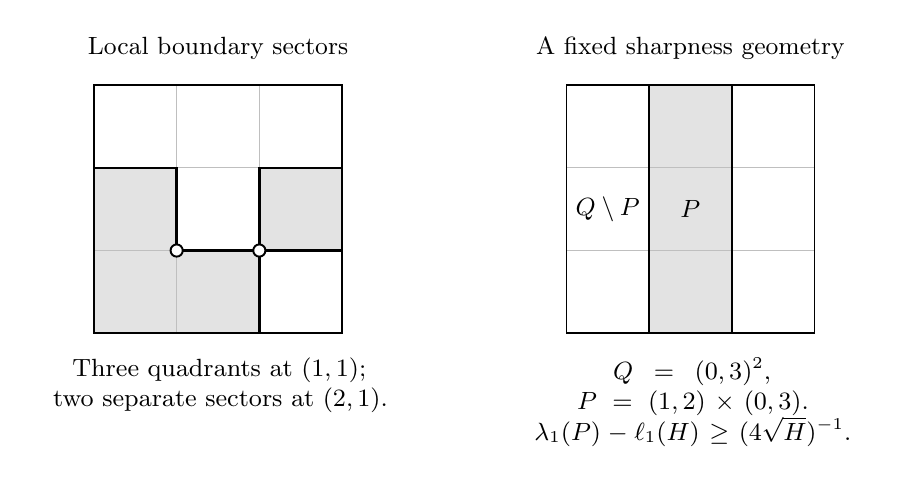
\begin{tikzpicture}[x=1.05cm,y=1.05cm,font=\small,>=Stealth]
 \begin{scope}
  \fill[gray!22] (0,0) rectangle (2,1);
  \fill[gray!22] (0,1) rectangle (1,2);
  \fill[gray!22] (2,1) rectangle (3,2);
  \draw[step=1,gray!50,line width=.35pt] (0,0) grid (3,3);
  \draw[line width=.9pt] (0,0)--(2,0)--(2,1)--(1,1)
                          --(1,2)--(0,2)--cycle;
  \draw[line width=.9pt] (2,1) rectangle (3,2);
  \draw[line width=.6pt] (0,0) rectangle (3,3);
  \draw[fill=white,line width=.7pt] (1,1) circle[radius=2.2pt];
  \draw[fill=white,line width=.7pt] (2,1) circle[radius=2.2pt];
  \node[align=center] at (1.5,3.45) {Local boundary sectors};
  \node[anchor=north,align=center,text width=4.6cm] at (1.5,-.18)
       {Three quadrants at \((1,1)\);\\
        two separate sectors at \((2,1)\).};
 \end{scope}
 \begin{scope}[xshift=6cm]
  \fill[gray!22] (1,0) rectangle (2,3);
  \draw[step=1,gray!50,line width=.35pt] (0,0) grid (3,3);
  \draw[line width=.6pt] (0,0) rectangle (3,3);
  \draw[line width=.9pt] (1,0) rectangle (2,3);
  \node at (.5,1.5) {\(Q\setminus P\)};
  \node at (1.5,1.5) {\(P\)};
  \node[align=center] at (1.5,3.45) {A fixed sharpness geometry};
  \node[anchor=north,align=center,text width=4.4cm] at (1.5,-.18)
       {\(Q=(0,3)^2\),\\
        \(P=(1,2)\times(0,3)\).\\
        \(\lambda_1(P)-\ell_1(H)\ge(4\sqrt H)^{-1}\).};
 \end{scope}
\end{tikzpicture}
\caption{Clipping certificates use the actual open interior of the
shaded cells. Left: the bilinear boundary field has value \((1,1)\)
at the reentrant vertex \((1,1)\), but has two independent sector
values \((1,1)\) and \((-1,-1)\) at the point contact \((2,1)\).
These point values do not join the open components.
Right: the rectangular mask used in \eqref{cert:sharp-example}
shows that the \(H^{-1/2}\) clipping rate is already necessary on
one fixed geometry; the displayed lower bound holds for \(H\ge36\).}
\label{fig:mask-geometry}
\end{figure}



\subsection{A supplied conforming triangular mesh}
\label{cert:triangles}

Let a finite conforming straight-sided triangulation cover
$\overline Q$, and let $P$ be the interior of a nonempty union
of its selected closed triangles.  Assume every angle of every
ambient triangle is at least $\theta>0$ and every altitude is
at least $\sigma>0$.  These bounds include the unselected
triangles.  Set
\begin{equation}\label{cert:triangle-constant}
 A_\theta=\csc(\theta/2),\qquad B_\theta=\csc^2\theta,\qquad
 D_\theta=4\{24A_\theta(1+B_\theta)+2\}.
\end{equation}
We claim that
\begin{equation}\label{cert:triangle-rate}
 0\le\lambda_j(P)-\ell_j(H)
 \le D_\theta(E+\sigma^{-2})^{3/2}H^{-1/2},
 \qquad \lambda_j(P)\le E,\quad H>0.
\end{equation}

First rescale so that every altitude is at least one.
At each boundary vertex assign a nodal value separately on
each occupied sector of opening $\omega$.  For $\omega\ne\pi$
solve $h\cdot n_1=h\cdot n_2=1$ for the two outward boundary
normals; its norm is $1/\sin(\omega/2)$.  For a flat sector use
the common normal, and at a full interior vertex use zero.
Every nonempty occupied sector and every missing sector at an
interior boundary vertex contains a triangle, so
$\theta\le\omega\le2\pi-\theta$.  At an ambient boundary vertex
the exterior of the square supplies the missing angle.
Thus all nodal values have norm at most $A_\theta$.

Interpolate affinely on each occupied triangle.  Across a shared
occupied edge the endpoint values agree, while contact sectors
are again independent.  Barycentric basis gradients have norm
at most one, the reciprocal of the respective altitudes.
Consequently
\[
 |h|\le A_\theta,\qquad \norm{Dh}_{\mathrm{op}}\le3A_\theta,
 \qquad|\operatorname{div}h|\le6A_\theta,\qquad h\cdot n=1.
\]
The corner exponent is
$\beta=\pi/\omega\ge\pi/(2\pi-\theta)>1/2$, so
Section~\ref{cert:corners} justifies \eqref{cert:rellich}.
For $s\ge1$ it follows that
\begin{equation}\label{cert:triangle-flux}
 \norm{\partial_n(A_P+s)^{-1}f}_{L^2(\Gamma)}^2
 \le A_\theta(s^{-1/2}+3s^{-1})\norm f_2^2
 \le4A_\theta s^{-1/2}\norm f_2^2 .
\end{equation}

For the exterior trace let $e$ be an exposed interior edge,
$T_e$ its adjacent empty triangle, $z$ the opposite vertex,
and $a_e$ the altitude to $e$.  If $L_{T_e}$ is the longest
side, then
\[
 L_{T_e}/a_e\le\csc^2\theta=B_\theta.
\]
Indeed, the sine law gives every side length at least
$L_{T_e}\sin\theta$, and the altitude is such a side times
the sine of a base angle, again at least $\sin\theta$.
The vector field $X_e(x)=(x-z)/a_e$ on $T_e$ has outward
normal component one on $e$ and zero on its other two edges,
with $\operatorname{div}X_e=2/a_e\le2$ and
$|X_e|\le B_\theta$.  The divergence theorem for $|v|^2X_e$
therefore gives
\[
 \int_e|v|^2\le2\int_{T_e}|v|^2+
       2B_\theta
        \left(\int_{T_e}|v|^2\int_{T_e}|\nabla v|^2\right)^{1/2}.
\]
Each empty triangle is charged at most three times.  With
$M=\int_{Q\setminus P}|v|^2$ and
$T=\int_{Q\setminus P}|\nabla v|^2$ this yields
\[
 \norm{\gamma v}_{L^2(\Gamma)}^2
 \le6M+6B_\theta\sqrt{MT}
 \le6(1+B_\theta)\kappa^{-1/2}a_{\kappa,s}(v),
 \qquad \kappa\ge1.
\]
Edges on $\partial Q$ have zero trace.
Thus \eqref{cert:geometric-inputs} holds with
$F=4A_\theta$ and $C=6(1+B_\theta)$.  Applying
\eqref{cert:general-gap} proves \eqref{cert:triangle-rate}
in the normalized geometry.

To restore physical units put $x=\sigma y$.  The transformed
energies are $E'=\sigma^2E$ and $H'=\sigma^2H$, and the
transformed eigenvalue difference is $\sigma^2(\lambda_j-\ell_j)$.
Hence
\[
 \lambda_j-\ell_j
 \le D_\theta\sigma^{-2}(\sigma^2E+1)^{3/2}
                                  (\sigma^2H)^{-1/2}
 =D_\theta(E+\sigma^{-2})^{3/2}H^{-1/2},
\]
as asserted.  A sufficient cutoff for error at most $\tau/2$ is
\begin{equation}\label{cert:triangle-cutoff}
 H\ge4D_\theta^2(E+\sigma^{-2})^3\tau^{-2}.
\end{equation}
The rectangle in \eqref{cert:sharp-example} has a fixed
right-triangle mesh, so the same $H$ exponent is sharp in this
larger class.  For rational vertices the complete arithmetic
construction is given in Appendix~\ref{arith:triangles}; the constants
retain their explicit dependence on the supplied mesh quality.

\subsection{The finite matrix as a whole-resolvent approximation}
\label{cert:whole-resolvent}

The clipped inverse has an identity plateau and is not compact.
The correct finite-rank approximation is obtained by subtracting
exactly that plateau.  Put $\kappa=H+s$, $R_{P,s}=(A_P+s)^{-1}$,
and
\begin{equation}\label{cert:finite-rank}
 F_{H,s}=(B_H+s)^{-1}-\kappa^{-1}I
        =\kappa^{-1}S_H(\kappa I-M_H)^{-1}S_H^*.
\end{equation}
The last formula follows from \eqref{cert:finite-gram}, or by
applying the scalar identity on each singular direction of
$S_H$.  Thus $F_{H,s}$ is positive and finite rank, determined
by the same Gram matrix and the known restricted ambient modes.

For unit masks, $s\ge1$ and $H>0$, define
\begin{equation}\label{cert:finite-rank-eta}
 \eta_{H,s}=\frac{60}{\sqrt{s(H+s)}}+\frac1{H+s}.
\end{equation}
The harmonic-mean comparison gives
\[
 0\le F_{H,s}\le J^*(K_\kappa+s)^{-1}J
                 \le J^*(A_Q+s)^{-1}J.
\]
Together with $(B_H+s)^{-1}\ge R_{P,s}$ and
\eqref{cert:penalty-resolvent}, this yields
\[
 -\kappa^{-1}I\le F_{H,s}-R_{P,s}\le\eta_{H,s}I,
 \qquad
 \norm{F_{H,s}-R_{P,s}}_{\mathrm{op}}\le\eta_{H,s}.
\]
For a planar finite-area Dirichlet domain $G$, free heat
domination gives
\[
 N_{(A_G+s)^{-1}}(t)
 \le N_{A_G}(1/t)
 \le e\,\operatorname{Tr}(e^{-tA_G})
 \le\frac e{4\pi}|G|t^{-1},\qquad t>0,
\]
where the left count uses eigenvalues strictly greater than $t$
and the middle count uses energies below the stated threshold.
Compression does not increase ordered positive eigenvalues.
For the compact self-adjoint error
$D=F_{H,s}-R_{P,s}$, its positive eigenvalues are bounded by
those of $F_{H,s}$ and its negative magnitudes by those of
$R_{P,s}$.  Therefore
\[
 N_{|D|}(t)\le\frac e{4\pi}(|P|+|Q|)t^{-1},
 \qquad N_{|D|}(t)=0\quad(t>\eta_{H,s}).
\]
Integration of this count proves, for every $p>1$,
\begin{equation}\label{cert:finite-rank-schatten}
 \boxed{\quad
 \norm{F_{H,s}-R_{P,s}}_{\mathcal S_p}^{p}
 \le\frac p{p-1}\frac e{4\pi}(|P|+|Q|)
                                  \eta_{H,s}^{p-1}.
 \quad}
\end{equation}
Thus the finite hierarchy approximates the entire shifted
resolvent in every planar Schatten class above its summability
threshold.  For nonempty $P$ the threshold is strict: an interior
square already forces the Dirichlet inverse to lie outside
$\mathcal S_p$ for $0<p\le1$, and a finite-rank perturbation
cannot remove this tail.  Without plateau subtraction the error
is $\kappa^{-1}I$ plus a compact operator, hence is noncompact
for every finite $H$.

For triangular masks the same assertions hold for
$s\ge\sigma^{-2}$ after replacing \eqref{cert:finite-rank-eta} by
\[
 \eta_{H,s;\theta,\sigma}
 =\frac{24\csc(\theta/2)(1+\csc^2\theta)}
          {\sqrt{s(H+s)}}+\frac1{H+s}.
\]
Under $x=\sigma y$, the normalized resolvent is multiplied by
$\sigma^2$ on returning to physical units, while $H$ and $s$
both acquire the factor $\sigma^2$.  These factors give exactly
the displayed expression; the areas in
\eqref{cert:finite-rank-schatten} are physical areas.
The Schatten rate here follows from the counting bound and is
not asserted to be sharp.



\section{Effective optimization and finite checks}\label{sec:effective}

The preceding constructions separate three costs: the size of the
geometric library, the cutoff needed for each continuum spectrum,
and the arithmetic precision of its finite matrix.  We now combine
them into value enclosures and witnesses.  No comparison of two
exact eigenvalues is required.

For the exact-index problem, let a dyadic tolerance
\(0<\varepsilon\le1\) be given.  Use the boundary-filtered library
of \eqref{grid:exact-index-budget} and
\eqref{boundary:exact-index} with \(\gamma=\varepsilon/4\).
Write \(M\) for its true minimum.  Enclose each candidate's
normalized \(k\)-th eigenvalue in a rational interval of width
at most \(\eta=\varepsilon/4\), using
Section~\ref{sec:certification} and Appendix~\ref{arith:section}.
The minima \(l,u\) of the lower and upper endpoints satisfy
\[
 l\le M\le u,\qquad u-l\le\eta.
\]
For the width assertion, use the candidate attaining \(l\):
its upper endpoint is at most \(l+\eta\), and \(u\) is no
larger.  Equation~\eqref{grid:exact-index-value} gives the
fully rational enclosure
\begin{equation}\label{effective:mu-interval}
 \mu_k\in\left[\frac{l}{1+\gamma},\,u\right].
\end{equation}
Its lower endpoint is positive.  Indeed,
\(l\ge M-\eta\ge2\pi k-\eta>23/4\).
The ratio of the upper endpoint to the lower endpoint is at most
\[
 (1+\gamma)\frac ul
 \le 1+\gamma+(1+\gamma)\frac{\eta}{l}
 <1+\left(\frac14+\frac5{92}\right)\varepsilon
 <1+\varepsilon.
\]
Thus this is a relative enclosure with the requested accuracy,
including all multiplicities and without assuming that the
domain infimum is attained.  A candidate attaining the least
upper endpoint also satisfies
\[
 \lambda_k(P_*^\#)\le u\le M+\eta
 \le(1+\gamma)\mu_k+\eta<(1+\varepsilon)\mu_k,
\]
so the computation returns an actual approximate minimizing domain.

For the all-index problem use the connected, boundary-filtered
catalogue with \(\gamma=\varepsilon/64\) and its index budget
\(J_\gamma\).  Enclose each ratio
\(\abs P\lambda_j(P)/j\) to width at most
\(\eta=\varepsilon/4\).  Enclosing the corresponding normalized
eigenvalue to width \(\eta\) is sufficient since \(j\ge1\).
The same minimum-endpoint construction yields
\begin{equation}\label{effective:L-interval}
 L\in\left[\frac{l}{1+\gamma},\,u\right].
\end{equation}
Here \(M\le(1+\gamma)L\), so
\[
 u-\frac{l}{1+\gamma}
 \le\eta+\frac{\gamma l}{1+\gamma}
 \le\eta+\gamma L
 \le\frac{\varepsilon}{4}
       +\frac{4\pi\varepsilon}{64}<\frac{\varepsilon}{2}.
\]
A least-upper-endpoint candidate is within the same additive
allowance of \(L\).  In particular, \eqref{effective:L-interval}
computes the real number \(L\) to arbitrary absolute accuracy.

Boundary-edge reconstruction and validity tests use polynomial
time in the containing grid dimensions.  The proof of
Appendix~\ref{arith:section} gives polynomial per-mask bit cost
in \(B,m,\tau^{-1}\), with all continuum and arithmetic errors
included.  Substituting the catalogue budgets and multiplying
by their candidate counts gives deterministic bit-cost upper bounds
\begin{equation}\label{effective:costs}
 \exp\!\left(O\!\left(k^2\varepsilon^{-1}
                         \log\frac{2k}{\varepsilon}\right)\right),
 \qquad
 \exp\!\left(O\!\left(\varepsilon^{-5}
                         \log\frac2\varepsilon\right)\right)
\end{equation}
for \eqref{effective:mu-interval} and
\eqref{effective:L-interval}, respectively.
The constants are absolute for these scalar tasks.
The second search includes its \(J_\gamma\) indices; their
polynomial factor is absorbed by the displayed bound.
These estimates use a binary encoding of \(k\) and a dyadic
accuracy request.  An arbitrary rational input tolerance can
first be rounded down to a dyadic number within a factor two,
charging the input's bit length separately.
For a general computable objective, the additional cost of its
supplied evaluation algorithm remains a separate parameter,
as in Section~\ref{sec:objectives}.



\appendix


\section{Certified arithmetic and per-mask bit bounds}
\label{arith:section}

The continuum estimates in Section~\ref{sec:certification} give
an a-priori stopping cutoff.  This appendix specifies the
arithmetic needed to turn that cutoff into rational intervals.
For packed unit-cell masks it also proves polynomial per-mask
bit cost in the numerical parameters $B,m,\tau^{-1}$.  For a
supplied rational triangular mesh the conclusion is termination
with an explicit dimension and error budget.

\subsection{Unit-cell Gram entries and arithmetic error}
\label{arith:one-mask}

Let a nonempty raw mask $P$ have $n_P\le B$ cells in the
packed square $Q=(0,b)^2$, $b=2B$.  Fix a prefix length $m\ge1$
and a dyadic tolerance $0<\tau\le1$ for its unit-area
normalization.  Put
\begin{equation}\label{arith:square-cutoff}
 t=\tau/B,\qquad E=30m,\qquad
 c=\left\lceil\frac{2^{20}}9 B^4(E+1)^3\tau^{-2}\right\rceil,
 \qquad f=\frac{\pi^2}{b^2}.
\end{equation}
By \eqref{cert:catalogue-cutoff}, the raw continuum error is
at most $t/2$.  The correction matrix $T_c$ from
\eqref{cert:integer-cutoff} has dimension
$N_c<c=O(B^4m^3\tau^{-2})$ and satisfies $0\le T_c\le cI$.

In normalized square coordinates, define
\[
 J_{pr}(a,d)=2\int_a^d\sin(p\pi x)\sin(r\pi x)\,\dd x .
\]
For $p\ne r$ this is
\begin{equation}\label{arith:sine-integrals}
 \left[
   \frac{\sin((p-r)\pi x)}{(p-r)\pi}
  -\frac{\sin((p+r)\pi x)}{(p+r)\pi}
 \right]_a^d,
\end{equation}
whereas for $p=r$ it is
\[
 (d-a)-\frac{\sin(2p\pi d)-\sin(2p\pi a)}{2p\pi}.
\]
Each Gram entry $G_{(p,q),(r,s)}$ is the sum over occupied cells
of the corresponding products of two such integrals.
The endpoints are rational.  The separate diagonal expression
handles repeated frequencies exactly.

For reference, an elementary rational enclosure for $\pi$ is
provided by
\begin{equation}\label{arith:machin}
 \pi=16\arctan(1/5)-4\arctan(1/239).
\end{equation}
The identity follows from the tangent addition formula:
$\tan(4\arctan(1/5))=120/119$ and
$\tan(4\arctan(1/5)-\arctan(1/239))=1$, with the latter
angle in $(0,\pi/2)$.  Alternating arctangent series have
next-term remainder bounds.  Before evaluating a sine, reduce
its rational multiple of $\pi$ modulo two and use reflection
to put the argument in $[-\pi/2,\pi/2]$.  The sine Taylor
polynomial with its Lagrange remainder then gives rational
outward intervals.  Integer square roots or rational bisection
enclose each $\sqrt{w_a}$.

Assemble outward intervals for $T_c$, preserve symmetry, and
round their midpoints to one common dyadic denominator,
including that rounding in the radii.  If $A$ is the resulting
rational symmetric midpoint matrix and $r_{ab}$ are its entry
radii, then
\begin{equation}\label{arith:matrix-radius}
 \norm{T_c-A}_{\mathrm{op}}
 \le\Delta:=\max_a\sum_b r_{ab}.
\end{equation}
The matrix dimension is thus explicitly included in the
rounding budget.

Here is one concrete allocation of the raw tolerance $t$.
Choose a positive rational interval $[f_-,f_+]$ containing $f$,
and refine the matrix and scalar intervals until
\begin{equation}\label{arith:square-budget}
 \Delta\le\frac{t}{16f_+},\qquad
 f_+-f_-\le\frac{t}{8c}.
\end{equation}
Enclose each required decreasing eigenvalue of $A$ in a rational
interval of width
$\zeta\le t/(8f_+)$.  Enlarging by $\Delta$ on each side gives
an interval for $\nu_j(T_c)$; intersect it with $[0,c]$.
The width is at most $\zeta+2\Delta$.
Inserting this interval and $[f_-,f_+]$ in
\eqref{cert:integer-cutoff} gives a rational interval
$[L_j,U_j]$ for $\ell_j(c)$, of width at most
\[
 f_+(\zeta+2\Delta)+c(f_+-f_-)
 \le\frac t4+\frac t8=\frac{3t}{8}.
\]
Zero continuation is used if the index exceeds $N_c$.
Adding the one-sided continuum allowance gives
\begin{equation}\label{arith:square-output}
 \lambda_j(P^\#)\in
 [\,n_PL_j,\ n_P(U_j+t/2)\,],\qquad 1\le j\le m,
\end{equation}
with width at most $7\tau/8<\tau$.
The use of $2\Delta$, rather than $\Delta$, in this interval
width accounts for the possible overhang of an outward
endpoint.

\subsection{Exact inertia and polynomial bit cost}
\label{arith:inertia}

We next give a deterministic eigenvalue procedure, so that no
success assumption about floating-point eigenvectors enters
\eqref{arith:square-output}.  For a rational symmetric matrix
$A$ and a dyadic shift $a$, compute the inertia of $A-aI$ by
symmetric rational elimination.  A nonzero diagonal entry is
used as a one-by-one pivot.  If every diagonal is zero but the
matrix is not zero, a nonzero off-diagonal entry gives, after
permutation, the invertible pivot
\[
 C=\begin{pmatrix}0&b\\ b&0\end{pmatrix},
\]
whose inertia has one positive and one negative direction.
If the remaining matrix is zero, its entire dimension is
nullity.  At each nonzero pivot,
\[
 \begin{pmatrix}C&F\\ F^T&G\end{pmatrix}
 \quad\text{is congruent to}\quad
 \begin{pmatrix}C&0\\0&G-F^TC^{-1}F\end{pmatrix}.
\]
Congruence is an invertible change of coordinates in a real
quadratic form and preserves inertia.  The pivot inertia
therefore adds to that of the smaller Schur complement.
There are at most $N_c$ stages and $O(N_c^3)$ rational
operations.

To control bit growth, clear the common dyadic denominator of
the original shifted matrix and suppose its integer entries
have at most $L_0$ bits.  Each later Schur-complement entry is
a bordered minor divided by the determinant of the previously
selected nonsingular principal block, with the initial scaling
restored.  This follows directly from the block determinant
formula; after either pivot size, the selected original
principal block remains nonsingular because its determinant
is the product of the invertible pivot determinants.
Hadamard's inequality bounds every determinant of order at
most $N_c$ by
\[
 N_c^{N_c/2}2^{N_cL_0}.
\]
Its binary length is
$O(N_c(L_0+\log(N_c+1)))$.  Reducing intermediate fractions by
their integer greatest common divisors therefore keeps all
stored entries at polynomial bit length.  The products and
sums in one elimination step also have polynomial bit length.
An arbitrarily small nonzero real pivot creates no difficulty:
its reciprocal remains a ratio of integers with the stated
bit bounds.

A rational row-sum bound gives a dyadic interval $[-R,R]$
containing the spectrum of $A$.  At a midpoint $a$, inertia
gives the number of eigenvalues at most $a$ as the negative
count plus the nullity of $A-aI$.  For the $j$th increasing
eigenvalue, retain the upper half of its bracket if that count
is less than $j$, and the lower half otherwise.  This remains
valid when $a$ is exactly an eigenvalue.  After
\[
 O\left(1+\log\frac{R+1}{\zeta}\right)
\]
inertia computations the bracket has width at most $\zeta$.
Decreasing indices are obtained by reversing the order.
The method counts multiplicities and requires no lower bound
on a spectral gap.  Computing all $N_c$ indices separately
still has polynomial bit cost.

For completeness, the construction of $A$ also has the
required polynomial bound.  Cell endpoints and active mode
indices have $O(\log(B+1)+\log(c+1))$ bits.
The reduction of sine arguments is exact rational arithmetic.
For a precision parameter $P_0$, a constant multiple of
$P_0+1$ terms in the series above suffices for $P_0$ output
bits.  Direct rational summation is enough: the products of
the factorial and integer denominators have polynomial bit
length.  Square-root enclosures have polynomial cost in
$P_0+\log(c+1)$.  Off-diagonal frequency denominators in
\eqref{arith:sine-integrals} are nonzero integers times $\pi$,
and $\pi>3$.

Summing over at most $B$ cells, multiplying weights bounded
by $c$, and applying the row-sum estimate over $N_c<c$ entries
lose only polynomial factors in $B,c$.  Thus a common precision
\begin{equation}\label{arith:entry-precision}
 P_0=O\left(1+\log(B+1)+\log(c+1)+\log(1/\tau)\right)
\end{equation}
suffices for \eqref{arith:square-budget} and the chosen
eigenvalue width.  Algorithmically, double $P_0$ until the
explicit outward inequalities hold.  The stated bound proves
that this refinement terminates within polynomial bit cost.
The bisection shifts also have polynomial bit length, so the
minor bound applies at every inertia call.  With
$c=O(B^4m^3\tau^{-2})$, this proves that
\eqref{arith:square-output} is computable using a number of
bit operations polynomial in $B,m,\tau^{-1}$.

This is a numerical-parameter bound in the ordinary binary
model: for $\tau=2^{-s}$ it is not asserted to be polynomial
in $s$.  Multiplying this per-mask polynomial by the finite
catalogue size leaves the outer exponential enumeration orders
unchanged.

\subsection{Effective certificates for a rational triangular mesh}
\label{arith:triangles}

The input now consists of a nondegenerate rational-vertex
square, a finite conforming triangulation of its closure with
rational vertices, a nonempty selection of triangles, an
integer $m\ge1$, and a positive rational $\tau$.
We show that rational intervals of width at most $\tau$ for
$\lambda_1(P),\ldots,\lambda_m(P)$ are computable.
The proof supplies explicit mesh-quality certificates and
entrywise errors, including all frequency coincidences.

Input validity is decidable by finite rational tests.
Determinants check orientation and nondegeneracy; the square
side vectors must have equal positive squared lengths and
zero dot product.  Check that all triangles lie in the closed
square, that pairwise intersections are empty or a whole common
edge or a common vertex, and that their areas sum to the square
area.  These conditions imply a conforming cover.  Indeed, a
missing interior point of their finite closed union would
have a neighborhood of positive area; boundary coverage follows
by closure.

At a triangle vertex let $e,f$ be the outgoing edge vectors
and $\Delta=|\det(e,f)|>0$.  The squared sine of its angle is
the positive rational number $\Delta^2/(|e|^2|f|^2)$.
Successive halving finds positive dyadic rationals $\theta,\sigma$
such that
\begin{equation}\label{arith:quality}
 \theta\le1,\qquad
 \theta^2\le\min_{e,f}\frac{\Delta^2}{|e|^2|f|^2},\qquad
 \sigma^2\le\min_{T,e}\frac{\Delta_T^2}{|e|^2}.
\end{equation}
The last expression is the squared altitude to $e$.
All minima include empty triangles.  Since
$\sin\alpha\ge\theta$ and $\sin\alpha\le\alpha$, every angle
is at least $\theta$ radians.  No inverse trigonometric
computation is needed.

Set the rational majorants
\begin{equation}\label{arith:constant-majorant}
 \overline A=\frac4\theta,\qquad
 \overline B=\frac4{\theta^2},\qquad
 \overline D=4\{24\overline A(1+\overline B)+2\}.
\end{equation}
The inequality $\sin x\ge2x/\pi$ on $[0,\pi/2]$, together
with $\pi<4$ and $\theta\le1$, gives
$D_\theta\le\overline D$.
An automatic rational ceiling for the first $m$ energies is
\begin{equation}\label{arith:triangle-ceiling}
 E=270m\sigma^{-2}.
\end{equation}
Indeed, the centroid of one occupied triangle is at distance
at least $\sigma/3$ from each supporting edge.  The
coordinate-aligned square of side $\sigma/3$ centered there
lies strictly in the triangle.  It has rational vertices.
Scaling the square estimate \eqref{cert:linear-ceiling} gives
$\lambda_m(P)<270m\sigma^{-2}$.

Write the possibly rotated square as
\[
 Q=\{o+t v+u w:0<t,u<1\},\qquad
 v\cdot w=0,\quad |v|^2=|w|^2=L^2>0,
\]
where $o,v,w$ are rational.  Every mesh vertex has rational
$(t,u)$ coordinates, $L^2$ is rational, and the absolute
Jacobian is $L^2$.  The ambient eigenfunctions are
$\phi_{kl}=2L^{-1}\sin(k\pi t)\sin(l\pi u)$.
Choose
\begin{equation}\label{arith:triangle-cutoff}
 c=\max\left\{3,\
    \left\lceil
       \frac{4L^2\overline D^2(E+\sigma^{-2})^3}
                       {9\tau^2}
    \right\rceil\right\},
 \qquad H=\frac{\pi^2c}{L^2}.
\end{equation}
By \eqref{cert:triangle-cutoff} and $\pi^2>9$, the continuum
error is at most $\tau/2$.  The active list
$\mathcal I_c=\{(k,l)\in\N^2:k^2+l^2<c\}$ is obtained by
integer comparisons and has size $1\le N_c\le\pi c/4<c$.
Put
\[
 r_a=k_a^2+l_a^2,\quad d_a=\sqrt{c-r_a},\quad
 q=\pi^2/L^2,\quad
 G_{ab}=\int_P\phi_a\phi_b,\quad M_{ab}=q\,d_ad_bG_{ab}.
\]
Then $M$ is the physical Gram correction matrix $M_H$ and
$\ell_j(H)=H-\nu_j(M)$, with zero continuation beyond $N_c$.
Although $L$ need not be rational, its two normalization
factors cancel the area Jacobian in each Gram entry.

\subsection{Triangle integration without singular denominators}
\label{arith:triangle-integrals}

In the normalized $(t,u)$ coordinates the integrand of
$G_{ab}$ is
$4\sin(k\pi t)\sin(k'\pi t)\sin(l\pi u)\sin(l'\pi u)$.
For a normalized triangle $T$ of rational area $A$ and rational
vertices $x_0,x_1,x_2$, consider an affine phase
$z(t,u)=a t+b u$ with integers $a,b$, and put $z_i=z(x_i)$.
The barycentric moment formula is
\[
 \int_T\lambda_0^i\lambda_1^j\lambda_2^k
 =\frac{2A\,i!j!k!}{(i+j+k+2)!}.
\]
It follows by the affine change from the standard simplex
and successive one-dimensional beta integrals; for integer
powers those integrals are obtained by repeated integration
by parts.  Define the rational polynomial
$h_r(z_0,z_1,z_2)=\sum_{i+j+k=r}z_0^iz_1^jz_2^k$.
Expanding the affine phase and its exponential gives the
absolutely convergent identity
\begin{equation}\label{arith:triangle-series}
 \int_T e^{i\pi z(t,u)}\,\dd t\,\dd u
 =2A\sum_{r=0}^{\infty}
           \frac{(i\pi)^r}{(r+2)!}h_r(z_0,z_1,z_2).
\end{equation}
In particular, no differences $z_i-z_j$ occur in a denominator.
Repeated phases, zero frequencies, and phases constant along
an edge are covered by the same formula.

For real $y$, the integral Taylor remainder gives
$|e^{iy}-\sum_{r=0}^{K}(iy)^r/r!|
\le|y|^{K+1}/(K+1)!$.
An affine phase stays between its vertex extrema.  With
$Z=\max_i|z_i|$, the error in truncating
\eqref{arith:triangle-series} at $K$ is therefore at most
\begin{equation}\label{arith:triangle-remainder}
 A\frac{(4Z)^{K+1}}{(K+1)!},
\end{equation}
using $\pi<4$.  The same estimate holds for the real part
$C_T(a,b)=\int_T\cos(\pi(at+bu))$.

Set $a_-=k-k'$, $a_+=k+k'$, $b_-=l-l'$,
$b_+=l+l'$, and $\epsilon_-=1,\epsilon_+=-1$.
Twice using product-to-sum gives the triangle contribution
\begin{equation}\label{arith:cosine-assembly}
 G_{ab}^{(T)}
 =\frac12\sum_{\rho,\sigma\in\{-,+\}}
     \epsilon_\rho\epsilon_\sigma
       \{C_T(a_\rho,b_\sigma)+C_T(a_\rho,-b_\sigma)\}.
\end{equation}
The total absolute coefficient of these eight terms is four.
For active modes and normalized vertices in $[0,1]^2$,
$|a_\rho|+|b_\sigma|\le4\sqrt c\le4c$.
The selected normalized area is at most one.
Hence the polynomial $P_{ab,K}(\pi)$ obtained by truncation
satisfies the uniform rational bound
\begin{equation}\label{arith:gram-remainder}
 |G_{ab}-P_{ab,K}(\pi)|
 \le4\frac{(16c)^{K+1}}{(K+1)!}.
\end{equation}
This tends to zero effectively.  To obtain error at most
$\eta$, increase $K$ until the right side is at most $\eta/2$,
then use \eqref{arith:machin} and rational interval polynomial
evaluation until the value interval has width at most $\eta$.
Its midpoint approximates $G_{ab}$ within $\eta$.
For a fixed polynomial the interval width tends to zero
as the input interval shrinks, so both refinements terminate.

\subsection{Rational matrix error and multiple eigenvalues}
\label{arith:triangle-errors}

An explicit common tolerance can be chosen before the
approximations.  Put $Q_0=16/L^2$, so $0<q<Q_0$, and set
\begin{equation}\label{arith:triangle-entry-budget}
 \eta=\min\left\{1,\frac{\tau}{12c},
       \frac{\tau}{48N_c(Q_0+1)(c+1)^2}\right\}.
\end{equation}
Compute rational approximations $\widehat q,\widehat d_a,
\widehat G_{ab}$ with absolute errors at most $\eta$.
For the square roots, bisection of $x^2-(c-r_a)$ on $[0,c]$
suffices.  Compute one Gram approximation for each unordered
pair and reflect it, preserving exact symmetry.  Define
$h=c\widehat q$ and
$\widehat M_{ab}=\widehat q\,\widehat d_a\widehat d_b
\widehat G_{ab}$.  Then $|H-h|\le\tau/12$.
Since $|G_{ab}|\le1$, $d_a\le c$,
$|\widehat d_a|\le c+1$ and
$|\widehat q|\le Q_0+1$, a four-term telescoping expansion gives
\[
 |M_{ab}-\widehat M_{ab}|
 \le\eta\{c^2+(Q_0+1)c+(Q_0+1)(c+1)
                              +(Q_0+1)(c+1)^2\}
 \le\frac{\tau}{12N_c}.
\]
Therefore
\begin{equation}\label{arith:triangle-norm-error}
 \norm{M-\widehat M}_{\mathrm{op}}
 \le\norm{M-\widehat M}_{\mathrm F}
 \le N_c\max_{a,b}|M_{ab}-\widehat M_{ab}|
 \le\tau/12.
\end{equation}
The approximate matrix need not be positive.  Symmetry and
the norm error suffice for ordered eigenvalue comparison.

For a fully elementary terminating procedure, compute the
characteristic polynomial of $\widehat M$ by exact rational
arithmetic, perform its square-free factorization, and use
Sturm isolation for its real roots.  Symmetry ensures that
all roots are real.  Refine each distinct-root interval to
width at most $\tau/6$; its midpoint has error at most
$\tau/12$.  Roots at subdivision endpoints are detected by
exact substitution and treated as exact roots.  The
multiplicities recovered from square-free factorization give
the ordered list, without an a-priori separation assumption.
The exact inertia procedure above is an alternative.

Let $\rho_j$ be the resulting midpoint for the $j$th decreasing
eigenvalue of $\widehat M$, repeated with multiplicity, and
continue $\rho_j=0$ for $j>N_c$.  By
\eqref{arith:triangle-norm-error},
$|\rho_j-\nu_j(M)|\le\tau/6$ for $j\le N_c$; beyond $N_c$
both continued corrections are zero.  Thus
$a_j=h-\rho_j$ satisfies $|a_j-\ell_j(H)|\le\tau/4$.
Adding the continuum allowance proves
\begin{equation}\label{arith:triangle-output}
 \boxed{\quad
 \lambda_j(P)\in
 [\,a_j-\tau/4,\ a_j+3\tau/4\,],\qquad 1\le j\le m.
 \quad}
\end{equation}
These intervals have width $\tau$ and handle repeated levels.

The construction is finite and every numerical assertion is
checkable by rational operations: one may retain the input
geometry tests, $\theta,\sigma$, the cutoff inequality,
Taylor orders and remainders, scalar enclosures, the symmetric
rational matrix, and the root counts.  Its matrix dimension is
\[
 O\bigl(1+L^2\overline D^2(E+\sigma^{-2})^3\tau^{-2}\bigr),
\]
or $O(1+L^2\overline D^2m^3\sigma^{-6}\tau^{-2})$ with
\eqref{arith:triangle-ceiling}.  The global Taylor expansion
was chosen to establish effectivity uniformly through phase
degeneracies.  No polynomial bit bound for this triangular
implementation is needed or asserted.

\subsection{Complete-basis checks and optional conforming upper bounds}
\label{arith:proposal-checks}

Exact inertia proves bounded per-mask computation.  For
independently checking numerical proposals, a complete-basis
residual test is also useful.  Let $A$ be rational symmetric,
$Q_0$ a rational square matrix of proposed eigenvectors, and
$D_0$ a diagonal matrix of ordered rational proposals.
Suppose exact rational norm bounds verify
\[
 g\ge\norm{Q_0^TQ_0-I}_{\mathrm{op}},\quad g<\tfrac12,
 \qquad r\ge\norm{AQ_0-Q_0D_0}_{\mathrm{op}},\qquad
 d=\norm{D_0}_{\mathrm{op}}.
\]
Frobenius bounds may be used throughout.  For a symmetric
matrix, the maximum absolute row sum also bounds its Euclidean
operator norm.  For the generally nonsymmetric residual
$R=AQ_0-Q_0D_0$, one may instead use
$\sqrt{\norm R_1\norm R_\infty}$, where these are the maximum
absolute column and row sums.  With $G=Q_0^TQ_0$ and $K=Q_0^TAQ_0$,
$G\ge(1-g)I>0$, so $Q_0$ is invertible, and
\[
 \norm{K-D_0}_{\mathrm{op}}
 \le(1+g)r+gd.
\]
This follows by expanding
$K-D_0=Q_0^T(AQ_0-Q_0D_0)+(G-I)D_0$ and using
$\norm{Q_0}\le\sqrt{1+g}\le1+g$.
For any nonzero coefficient vector, comparing its generalized
Rayleigh quotient for $(K,G)$ with that for $(D_0,I)$ adds
at most another $gd$ in the numerator and divides by
$1-g$.  Min--max gives, at every ordered index,
\begin{equation}\label{arith:complete-basis}
 |\lambda_j(A)-(D_0)_{jj}|
 \le\frac{(1+g)r+2gd}{1-g}=:\eta_A .
\end{equation}
The same statement applies after reversing both ordered lists.
It certifies indices and multiplicities, not merely a nearby
eigenvalue for each vector.

If $A$ approximates $T_c$ with norm error $\Delta$, put
$E_A=\Delta+\eta_A$.  A proposal plus $E_A$ is an upper
endpoint for the corresponding decreasing correction
eigenvalue and therefore gives a lower endpoint in
\eqref{cert:integer-cutoff}.  The endpoint's possible overhang
is $2E_A$, not $E_A$: the proposal itself may already be
$E_A$ above the true value.  For an outward scalar interval
$[f_-,f_+]$ and dyadic output denominator $S_0$, a sufficient
total raw lower-endpoint arithmetic allowance is
\begin{equation}\label{arith:proposal-allowance}
 2f_+E_A+c(f_+-f_-)+\frac{f_+}{S_0}+\frac1{S_0}.
\end{equation}
The last two terms pay for rounding the correction coordinate
and the final product.  Clamping the correction endpoint to
$[0,c]$ and the final lower endpoint to $[0,\infty)$ preserves
validity.

For upper bounds, subdivide the mask cells conformingly and
use continuous piecewise affine functions with zero boundary
nodal values.  These are in the actual $H^1_0(P)$, including
at point-contact vertices.  The dyadic hierarchy is nested
and dense: first approximate by a compactly supported smooth
function and then interpolate on a sufficiently fine mesh.
Its full Ritz values decrease to $\lambda_j(P)$.  On a
rectangle with side scales $s_x,s_y$ divided into $n$ intervals
in each direction and split into right triangles, the local
stiffness and consistent mass entries are rational:
\[
 K_{ij}=\frac12\left(\frac{s_y}{s_x}b_i b_j+
                         \frac{s_x}{s_y}c_i c_j\right),
 \qquad
 M_{ij}=\frac{s_xs_y}{24n^2}
       \begin{cases}2,&i=j,\\1,&i\ne j.\end{cases}
\]
Here $b_i,c_i$ are the signed edge differences in the
reference unit right triangle.  Assembly uses the consistent
$L^2$ mass, which is positive definite on the free nodal
space.

More generally, for a rational full-column-rank trial matrix
$C$ form $G=C^TMC$ and $K=C^TK_{\rm mesh}C$ exactly.
If $g\ge\norm{G-I}_{\mathrm{op}}$, $g<1/2$, and
$e\ge\norm{K-D_0}_{\mathrm{op}}$, min--max gives, at indices
where $d_j-e>0$,
\begin{equation}\label{arith:ritz}
 \frac{d_j-e}{1+g}
 \le\operatorname{Ritz}_j(C)
 \le\frac{d_j+e}{1-g}.
\end{equation}
The upper endpoint bounds the continuum eigenvalue.
The lower endpoint bounds only the trial Ritz value and is
not used as a continuum lower bound.  A certified subspace
may improve a finite interval without being a complete
eigenbasis of the full finite-element matrix.

\section*{Note on AI Use}
The author declares the use of consumer-grade Gemini-3 and GPT-6 models for prior-art search, exploring and developing ideas and proofs, drafting and LaTeX typesetting; the author takes full and sole responsibility for all contents of this work.

\begin{thebibliography}{99}

\bibitem{Agbanusi2015}
I.~C.~Agbanusi,
Pseudo-differential operators, transmission problems and the large
coupling limit,
arXiv:1509.08363, 2015.
\href{https://arxiv.org/abs/1509.08363}{arXiv:1509.08363}.

\bibitem{AllenKriventsovNeumayer2025}
M.~Allen, D.~Kriventsov and R.~Neumayer,
Quantitative resolvent and eigenfunction stability for the
Faber--Krahn inequality,
arXiv:2504.13053v2 (2025).
\href{https://arxiv.org/abs/2504.13053v2}{arXiv:2504.13053v2}.

\bibitem{Ashbaugh2017}
M.~S.~Ashbaugh,
Universal inequalities for the eigenvalues of the Dirichlet Laplacian,
in \emph{Shape Optimization and Spectral Theory}, A.~Henrot (ed.),
De Gruyter Open, 2017, 282--324.
\href{https://doi.org/10.1515/9783110550887-008}{doi:10.1515/9783110550887-008}.

\bibitem{BarbatisBurenkovLamberti2010}
G.~Barbatis, V.~I.~Burenkov and P.~D.~Lamberti,
Stability estimates for resolvents, eigenvalues and eigenfunctions
of elliptic operators on variable domains,
in \emph{Around the Research of Vladimir Maz'ya II},
International Mathematical Series, vol.~12, Springer, 2010, 23--60.
\href{https://doi.org/10.1007/978-1-4419-1343-2_2}
{doi:10.1007/978-1-4419-1343-2\_2}.

\bibitem{BarbatisLamberti2012}
G.~Barbatis and P.~D.~Lamberti,
Spectral stability estimates for elliptic operators subject to
domain transformations with non-uniformly bounded gradients,
\emph{Mathematika} \textbf{58} (2012), 324--348.
\href{https://doi.org/10.1112/S0025579311002397}
{doi:10.1112/S0025579311002397};
\href{https://arxiv.org/abs/1101.2545}{arXiv:1101.2545}.

\bibitem{BritzEtAl2021}
T.~Britz, A.~Carey, F.~Gesztesy, R.~Nichols, F.~Sukochev and D.~Zanin,
The product formula for regularized Fredholm determinants,
\emph{Proc. Amer. Math. Soc. Ser. B} \textbf{8} (2021), 42--51.
\href{https://doi.org/10.1090/bproc/70}{doi:10.1090/bproc/70};
\href{https://arxiv.org/abs/2007.12834v3}{arXiv:2007.12834v3}.

\bibitem{BruneauCarbou2002}
V.~Bruneau and G.~Carbou,
Spectral asymptotic in the large coupling limit,
\emph{Asymptot. Anal.} \textbf{29} (2002), no.~2, 91--113.
\href{https://doi.org/10.3233/ASY-2002-476}{doi:10.3233/ASY-2002-476}.

\bibitem{Bucur2003}
D.~Bucur,
Regularity of optimal convex shapes,
\emph{J. Convex Anal.} \textbf{10} (2003), 501--516.
\href{https://journalofconvexanalysis.com/articles/jca1031/}{Journal article page}.

\bibitem{Bucur2012}
D.~Bucur,
Minimization of the $k$-th eigenvalue of the Dirichlet Laplacian,
\emph{Arch. Ration. Mech. Anal.} \textbf{206} (2012), 1073--1083.
\href{https://cvgmt.sns.it/paper/1792/}{Author-deposited article and bibliographic record}.

\bibitem{BucurEtAl2026}
D.~Bucur, J.~Lamboley, M.~Nahon and R.~Prunier,
Sharp quantitative stability of the Dirichlet spectrum near the ball,
\emph{Comm. Pure Appl. Math.} \textbf{79} (2026), 827--896.
\href{https://doi.org/10.1002/cpa.70021}{doi:10.1002/cpa.70021}.

\bibitem{BucurMazzoleni2015}
D.~Bucur and D.~Mazzoleni,
A surgery result for the spectrum of the Dirichlet Laplacian,
\emph{SIAM J. Math. Anal.} \textbf{47} (2015), 4451--4466.
\href{https://doi.org/10.1137/140992448}{doi:10.1137/140992448}.

\bibitem{ChengYang2007}
Q.-M.~Cheng and H.~Yang,
Bounds on eigenvalues of Dirichlet Laplacian,
\emph{Math. Ann.} \textbf{337} (2007), 159--175.
\href{https://doi.org/10.1007/s00208-006-0030-x}{doi:10.1007/s00208-006-0030-x}.

\bibitem{ColboisElSoufi2014}
B.~Colbois and A.~El~Soufi,
Extremal eigenvalues of the Laplacian on Euclidean domains and closed surfaces,
\emph{Math. Z.} \textbf{278} (2014), 529--546.
\href{https://doi.org/10.1007/s00209-014-1325-3}{doi:10.1007/s00209-014-1325-3}.

\bibitem{Dauge2018}
M.~Dauge,
\emph{Initiation into corner singularities},
lecture notes, Mini-courses in Mathematical Analysis,
University of Padova, 2--6 July 2018.
\href{https://events.math.unipd.it/minicorsi/sites/default/files/2017/DaugeCorso.pdf}
{Author's lecture notes}.

\bibitem{Davies1989}
E.~B.~Davies,
\emph{Heat Kernels and Spectral Theory},
Cambridge Tracts in Mathematics, vol.~92,
Cambridge University Press, 1989.
\href{https://doi.org/10.1017/CBO9780511566158}{doi:10.1017/CBO9780511566158}.

\bibitem{EvansGariepy2015}
L.~C.~Evans and R.~F.~Gariepy,
\emph{Measure Theory and Fine Properties of Functions},
revised edition, CRC Press, 2015.

\bibitem{FackKosaki1986}
T.~Fack and H.~Kosaki,
Generalized \(s\)-numbers of \(\tau\)-measurable operators,
\emph{Pacific J. Math.} \textbf{123} (1986), 269--300.
\href{https://msp.org/pjm/1986/123-2/pjm-v123-n2-p03-s.pdf}
{Publisher's article}.

\bibitem{FreitasLagacePayette2021}
P.~Freitas, J.~Lagac\'e and J.~Payette,
Optimal unions of scaled copies of domains and P\'olya's conjecture,
\emph{Ark. Mat.} \textbf{59} (2021), 11--51.
\href{https://doi.org/10.4310/ARKIV.2021.v59.n1.a2}{doi:10.4310/ARKIV.2021.v59.n1.a2}.

\bibitem{JiangLin2026}
R.~Jiang and F.~Lin,
P\'olya's conjecture up to $\varepsilon$-loss and quantitative estimates
for the remainder of Weyl's law,
\emph{Comm. Pure Appl. Math.} (2026), e70058.
\href{https://doi.org/10.1002/cpa.70058}{doi:10.1002/cpa.70058}.

\bibitem{KlarnerRivest1973}
D.~A.~Klarner and R.~L.~Rivest,
A procedure for improving the upper bound for the number of $n$-ominoes,
\emph{Canad. J. Math.} \textbf{25} (1973), 585--602.
\href{https://people.csail.mit.edu/rivest/pubs/KR73.pdf}{Author-hosted article}.

\bibitem{Leclerc2003}
B.~Leclerc,
The median procedure in the semilattice of orders,
\emph{Discrete Appl. Math.} \textbf{127} (2003), 285--302.
\href{https://doi.org/10.1016/S0166-218X(02)00211-1}
{doi:10.1016/S0166-218X(02)00211-1}.

\bibitem{LiuOishi2013}
X.~Liu and S.~Oishi,
Verified eigenvalue evaluation for the Laplacian over polygonal domains
of arbitrary shape,
\emph{SIAM J. Numer. Anal.} \textbf{51} (2013), 1634--1654.
\href{https://doi.org/10.1137/120878446}{doi:10.1137/120878446}.

\bibitem{LiYau1983}
P.~Li and S.-T.~Yau,
On the Schr\"odinger equation and the eigenvalue problem,
\emph{Comm. Math. Phys.} \textbf{88} (1983), 309--318.
\href{https://doi.org/10.1007/BF01213210}{doi:10.1007/BF01213210}.

\bibitem{LuttingerFriedberg1976}
J.~M.~Luttinger and R.~Friedberg,
Some functional inequalities, with application to Green's function,
\emph{Arch. Rational Mech. Anal.} \textbf{61} (1976), 187--195.
\href{https://www.osti.gov/servlets/purl/4482963}
{Author report}.

\bibitem{MazzoleniPratelli2013}
D.~Mazzoleni and A.~Pratelli,
Existence of minimizers for spectral problems,
\emph{J. Math. Pures Appl.} (9) \textbf{100} (2013), 433--453.
\href{https://doi.org/10.1016/j.matpur.2013.01.008}{doi:10.1016/j.matpur.2013.01.008}.

\bibitem{ParkEtAl2017}
C.~Park, J.-W.~Park, S.~Park, D.~Seon and M.~Ziegler,
Computable operations on compact subsets of metric spaces with
applications to Fr\'echet distance and shape optimization,
arXiv:1701.08402v2 (2017).
\href{https://arxiv.org/abs/1701.08402v2}{arXiv:1701.08402v2}.

\bibitem{Polya1961}
G.~P\'olya,
On the eigenvalues of vibrating membranes,
\emph{Proc. London Math. Soc.} (3) \textbf{11} (1961), 419--433.
\href{https://doi.org/10.1112/plms/s3-11.1.419}{doi:10.1112/plms/s3-11.1.419}.

\bibitem{RoslerStepanenko2024}
F.~R\"osler and A.~Stepanenko,
Computing eigenvalues of the Laplacian on rough domains,
\emph{Math. Comp.} \textbf{93} (2024), 111--161.
\href{https://doi.org/10.1090/mcom/3827}{doi:10.1090/mcom/3827}.

\bibitem{vanDenBerg2012}
M.~van den Berg,
Estimates for the torsion function and Sobolev constants,
\emph{Potential Anal.} \textbf{36} (2012), 607--616.
\href{https://doi.org/10.1007/s11118-011-9246-9}
{doi:10.1007/s11118-011-9246-9}.

\bibitem{vanDenBergDavies1989}
M.~van den Berg and E.~B.~Davies,
Heat flow out of regions in \(\R^m\),
\emph{Math. Z.} \textbf{202} (1989), 463--482.
\href{https://doi.org/10.1007/BF01221585}{doi:10.1007/BF01221585}.

\end{thebibliography}
\end{document}
